% spine = 0.0025 * 60 = 0.15
% Minimum Cover Width: Bleed + Back Cover Trim Size + Spine Width + Front Cover Trim Size + Bleed =  0.125" + 5" + 0.15" + 5" + .125" = 10.4''
% Minimum Cover Height: Bleed + Book Height Trim Size + Bleed = 0.125" + 8" + .125" = 8.25"
\documentclass[makeidx, 12pt, oneside, onecolumn, openright, final, svgnames, dvipsnames, extrafontsizes]{memoir}


\usepackage[mathjax]{lwarp}

\usepackage{pifont, dingbat}


\newcommand*\circnode[1]{\tikz[baseline=(char.base)]{%
            \node[shape=circle,fill=Olive!20,draw,inner sep=1.0pt] (char) {#1};}}

%\usepackage{smartdiagram}
%\usesmartdiagramlibrary{additions}


\usepackage{wrapfig2}
\usepackage{kantlipsum}

\title{Ancient Science Publishers}
%\setcounter{tocdepth}{1} % Include subsections in the \TOC.
%\setcounter{secnumdepth}{0} % Number down to chapters.
\setcounter{FileDepth}{0}
\booltrue{CombineHigherDepths}
\HTMLPageTop{\LinkPrevious}
\HTMLPageBottom{\LinkNext}
%\HTMLPageBottom{\LinkHome}

%\HTMLTitle{Ancient Science Publishers}



\CSSFilename{lwarp_sagebrush.css}

\usepackage[makeindex]{imakeidx} % hyper link index
\usepackage[colorlinks=true, linkcolor=ruddybrown, linktoc=all]{hyperref}% hyper link ToC

\PassOptionsToPackage{cmyk}{xcolor}
\usepackage{comment, calligra}
%\usepackage[paperheight=8.25in,paperwidth=10.4in,margin=0in]{geometry}
%\usepackage{pdfpages}
\usepackage{tikz, comment}
\usepackage{calligra, url, comment, amsmath, amsthm, etoolbox, amssymb, manfnt}
\usepackage{varwidth} % hyphenate texts in TikZ Node (back cover)
\usetikzlibrary{fadings, shadings, shadows, decorations, decorations.footprints, decorations.text, calc, positioning, mindmap,arrows, patterns, arrows.meta}
\usepackage{libertine}
\usepackage{fontspec}
%\usepackage[weather, misc]{ifsym}
%\usepackage{marvosym}
\usepackage{multido}
\usepackage{hologo, mflogo}
\usepackage[outline]{contour}
\usepackage{pdfrender}
\usepackage{pst-text}
\usepackage{pst-light3d}
\usepackage{pgfplots}
\pgfplotsset{width=5cm}
\usepackage{tikz-3dplot}
\usepackage{tkz-euclide}
\usepackage{tfrupee}
\usepgfplotslibrary{fillbetween}
\usepgfplotslibrary{polar}

%\usepackage{algorithm}
\usepackage{listings}


\setmainfont{Avant Garde}
\fontsize{0.05cm}{0.1cm}\selectfont

\usetikzlibrary{
  arrows,
  calc,
  fit,
  patterns,
  plotmarks,
  shapes.geometric,
  shapes.misc,
  shapes.symbols,
  shapes.arrows,
  shapes.callouts,
  shapes.multipart,
  shapes.gates.logic.US,
  shapes.gates.logic.IEC,
  circuits.logic.US,
  circuits.logic.IEC,
  circuits.logic.CDH,
  circuits.ee.IEC,
  datavisualization,
  datavisualization.formats.functions,
  er,
  automata,
  backgrounds,
  chains,
  topaths,
  trees,
  petri,
  mindmap,
  matrix,
  calendar,
  folding,
  fadings,
  shadings,
  spy,
  through,
  turtle,
  positioning,
  scopes,
  decorations.fractals,
  decorations.shapes,
  decorations.text,
  decorations.pathmorphing,
  decorations.pathreplacing,
  decorations.footprints,
  decorations.markings,
  shadows,
  shadows.blur,
  lindenmayersystems,
  intersections,
  fixedpointarithmetic,
  fpu,
  svg.path,
  external,
}


\newcommand*{\RaisedText}[1]{%
  \begingroup
    \leavevmode
    \rlap{\kern-1pt\raise.5pt\hbox{\color{White}#1}}%
    \rlap{\kern1pt\raise-.5pt\hbox{\color{black}#1}}%
    \hbox{#1}%
  \endgroup
}

\newcommand*{\RaisedTextNew}[1]{%
  \begingroup
    \leavevmode
    \rlap{\kern-.1pt\raise.1pt\hbox{%
      \pdfrender{
        TextRenderingMode=Stroke,
        LineWidth=.2pt,
        StrokeColor=white,
      }#1%
    }}%
    \rlap{\kern.1pt\raise-.1pt\hbox{%
      \pdfrender{
        TextRenderingMode=Stroke,
        LineWidth=.2pt,
        StrokeColor=black,
      }#1%
    }}%
    \rlap{%
      \pdfrender{
        TextRenderingMode=Stroke,
        LineWidth=.2pt,
      }#1%
    }%
    \hbox{#1}%
  \endgroup
}

\newfontfamily\hindifont[Script=Devanagari, BoldFont={Sahadeva}]{Nakula}
\newenvironment{hindi}{\hindifont}{\par}
\DeclareTextFontCommand{\texthindi}{\hindifont}

\tikzset{
  ld/.style={level distance=#1},lw/.style={line width=#1},
  level 1/.style={ld=4.5mm, trunk, lw=1ex ,sibling angle=60},
  level 2/.style={ld=3.5mm, trunk!80!leaf a,lw=.8ex,sibling angle=56},
  level 3/.style={ld=2.75mm,trunk!60!leaf a,lw=.6ex,sibling angle=52},
  level 4/.style={ld=2mm, trunk!40!leaf a,lw=.4ex,sibling angle=48},
  level 5/.style={ld=1mm, trunk!20!leaf a,lw=.3ex,sibling angle=44},
  level 6/.style={ld=1.75mm,leaf a, lw=.2ex,sibling angle=40},
}
\pgfarrowsdeclare{leaf}{leaf}{
  \pgfarrowsleftextend{-2pt} \pgfarrowsrightextend{1pt}
}{
  \pgfpathmoveto{\pgfpoint{-2pt}{0pt}}
  \pgfpatharc{150}{30}{1.8pt}
  \pgfpatharc{-30}{-150}{1.8pt}
  \pgfusepathqfill
}

\makeatletter
\def\agobble#1\nil#2{}
\def\mytextcolor@a#1 #2\nil#3{%
  \mytextcolor@b#1\nil{#3}
  \if\relax\detokenize{#2}\relax\expandafter\agobble\fi
  \mytextcolor@a#2\nil{#3}%
}
\def\mytextcolor@b#1#2\nil#3{%
  \textcolor{-#3}{\textbf{#1}}\textcolor{#3}{#2}\\
}
\def\mytextcolor#1#2{%
  \if\relax\detokenize{#2}\relax\expandafter\agobble\fi
  \mytextcolor@a#2 \nil{#1}%
}

\newcommand{\logo}[8]{%
  \colorlet{border}{#1}
  \colorlet{trunk}{#2}
  \colorlet{leaf a}{#3}
  \colorlet{leaf b}{#4}
%  \rotatebox{#8}{%
%    \begin{tikzpicture}[font=\scriptsize\scshape]
      \begin{scope}[scale=0.5, shift={(#8)}]
      \coordinate (root) [grow cyclic,rotate=90]
        child {
          child [line cap=round] foreach \a in {0,1} {
            child foreach \b in {0,1} {
              child foreach \c in {0,1} {
                child foreach \d in {0,1} {
                child foreach \leafcolor in {leaf a,leaf b}
                  { edge from parent [color=\leafcolor,-#5] }
                }
              }
            }
          }
          edge from parent [shorten >=-1pt,serif cm-,line cap=butt]
        };
      \node [scale=1,align=center,below,transform shape] at (0pt,-.5ex){%
        \mytextcolor{#6}{#7}\\
      };
    \end{scope}
%    \end{tikzpicture}
%  }
}
\makeatother


\tikzset{
    shade border west to east/.style args={#1 to #2}{
        preaction={draw, very thick, path fading=east, #1},
        preaction={draw, very thick, path fading=west, #2}
    },
    shade fill west to east/.style args={#1 to #2}{
        left color=#1,
        right color=#2
    }
}

\def\nodeshadowed[#1]#2;{\node[scale=0.45,above,#1]{#2};\node[scale=0.45,
        above,#1,yscale=-1,scope fading=south,opacity=0.0,yslant=0.0]{#2};}
        


%\definecolor{celestialblue}{rgb}{0.29, 0.59, 0.82}
\definecolor{celestialblue}{cmyk}{0.649, 0.274, 0.0, 0.164}

\definecolor{vividviolet}{rgb}{0.62, 0.0, 1.0}
\definecolor{satinsheengold}{rgb}{0.8, 0.63, 0.21}
\definecolor{darkorchid}{rgb}{0.6, 0.2, 0.8}
\definecolor{modebeige}{rgb}{0.59, 0.44, 0.09}

\newcommand{\hl}[1]{\textcolor{vividviolet}{#1}}% prints text in burntorange
\newcommand{\hlt}[1]{\textcolor{vividviolet}{\emph{#1}}}% prints italicized text in burntorange
\newcommand{\hlm}[1]{{\textcolor{modebeige}{#1}}}% prints math in Sepia
\newcommand{\hlbt}[1]{\textbf{\textcolor{Olive}{#1}}}% prints bold text in burntorange
%\newcommand{\hlmb}[1]{{\color{modebeige}{#1}}}% prints math in Sepia


% Inserts a blank page
\newcommand{\blankpage}{\newpage\hbox{}\thispagestyle{empty}\newpage}

\usepackage[mathcal]{euscript}
\newcommand{\conceptequiv}{\triangleq}
\CustomizeMathJax{\newcommand{\conceptequiv}{\triangleq}}
%\newcommand{\concepte}{\triangleq}
%\renewcommand{\models}{\looparrowright}
\renewcommand{\models}{\vDash}
\newcommand{\CC}{\mathcal{C}}
\CustomizeMathJax{\newcommand{\CC}{\mathcal{C}}}
\newcommand{\refines}{\looparrowright}
\CustomizeMathJax{\newcommand{\refines}{\looparrowright}}
\newcommand{\weakens}{\looparrowleft}
\CustomizeMathJax{\newcommand{\weakens}{\looparrowleft}}
\newcommand{\concept}[1]{\textcolor{Green}{#1}}

\newcommand\textproblem[1]{{\begin{center}\small \bfseries #1\end{center}}}


% no space ccenter
\newenvironment{nscenter}
 {\parskip=0pt\par\nopagebreak\centering}
 {\par\noindent\ignorespacesafterend}
 

\colorlet{LineColor}{White} 
\colorlet{FillColor}{Olive}%{DarkCyan}
%\colorlet{MyColor}{DarkOrange} 
%\colorlet{MyColor}{YellowOrange} 
\colorlet{MyColor}{Black}

\colorlet{TitleColor}{BurntOrange}
\colorlet{SubTitleColor}{Sepia}
\colorlet{DrawingTextColor}{Sepia}

\colorlet{AuthorTextColor}{Sepia}
\colorlet{BackTextColor}{Gray}
\colorlet{SpineTextColor}{Gray}

\colorlet{TriangleColor}{BurntOrange}
\colorlet{TriangleLineColor}{Sepia}
\colorlet{TriangleVertexColor}{Sepia}

\newcommand{\itemcolor}[1]{% Update list item colour
  \renewcommand{\makelabel}[1]{\color{#1}\hfil ##1}}
  
\newcommand\shadetext[2][]{%
  \setbox0=\hbox{{\special{pdf:literal 7 Tr }#2}}%
  \tikz[baseline=0]\path [#1] \pgfextra{\rlap{\copy0}} (0,-\dp0) rectangle (\wd0,\ht0);%
}

\newcommand{\aum}{\texthindi{ॐ}}
\newcommand{\Repeat}{\multido{\i=1+1}}

%\tikzfading[name=fade out,inner color=transparent!0,outer color=transparent!100]



\colorlet{EagleBodyColor}{White}
\colorlet{EagleHeadColor}{BurntOrange}
\colorlet{EagleEyeColor}{White}

\makeatletter
\tikzset{nomorepostaction/.code={\let\tikz@postactions\pgfutil@empty}}
\makeatother

\usepackage[capitalize,nameinlink]{cleveref}

\crefformat{chapter}{#2Dialogue~#1#3} % change cref to print Dialogue instead of Chapter

\newcommand\pr[1]{{\scshape\color{Black}\cref{#1}{ }(\cpageref{#1})}}
\newcommand\ar[1]{{\scshape\color{Black}\cref{#1}{ }(\cpageref{#1})}}
\newcommand\chref[1]{{\scshape\color{Black}\cref{#1}{ }(\cpageref{#1})}}

\newcommand\thmref[1]{{[\emph{\cref{#1}{ }(\cpageref{#1})}]}}
\newcommand\corref[1]{{[\emph{\cref{#1}{ }(\cpageref{#1})}]}}
\newcommand\exref[1]{{[\emph{\cref{#1}{ }(\cpageref{#1})}]}}

\definecolor{nicered}{rgb}{.647,.129,.149}
\definecolor{sanddune}{rgb}{0.59, 0.44, 0.09}
\definecolor{russet}{rgb}{0.5, 0.27, 0.11}
\makeatletter
\newlength\dlf@normtxtw
%\newcommand{\chapname}{Dialogue}
\setlength\dlf@normtxtw{\textwidth}
\def\myhelvetfont{\def\sfdefault{mdput}}
\newsavebox{\feline@chapter}
\newcommand\feline@chapter@marker[1][4cm]{%
  \sbox\feline@chapter{%
    \resizebox{!}{#1}{\fboxsep=1pt%
      \colorbox{sanddune}{\color{white}\bfseries\sffamily\thechapter}%
    }}%
  \rotatebox{90}{%
    \resizebox{%
      \heightof{\usebox{\feline@chapter}}+\depthof{\usebox{\feline@chapter}}}%
    {!}{\scshape\@chapapp}}\quad%
  \raisebox{\depthof{\usebox{\feline@chapter}}}{\usebox{\feline@chapter}}% 
}
\newcommand\feline@chm[1][4cm]{%
  \sbox\feline@chapter{\feline@chapter@marker[#1]}%
  \makebox[0pt][l]{% aka \rlap
    \makebox[0.0cm][r]{\usebox\feline@chapter}%
  }}
\makechapterstyle{daleif1}{
  \renewcommand\chapnamefont{\normalfont\Large\scshape\raggedleft\so}
  \renewcommand\chaptitlefont{\normalfont\huge\bfseries\scshape\color{Purple}}
  \renewcommand\chapternamenum{}
  \renewcommand{\chaptername}{Dialogue}
  %\renewcommand\printchaptername{\bfseries\color{DarkOrchid}}
  \renewcommand\printchaptername{\bfseries\color{russet}}
  \renewcommand\printchapternum{\null\hfill\feline@chm[2.5cm]\par}
  \renewcommand\afterchapternum{\par\vskip\midchapskip}
  \renewcommand\printchaptertitle[1]{\chaptitlefont\raggedleft ##1\par}
}
\makeatother

\setsecheadstyle{\normalfont\Large\bfseries\scshape\color{DarkOrchid}}


\chapterstyle{daleif1}
%\pagestyle{empty}

% Multi-page equations : mathmode by amsmath
\allowdisplaybreaks

\newenvironment{rcases}
  {\left.\begin{aligned}}
  {\end{aligned}\right\rbrace}
  
 \definecolor{ruddybrown}{rgb}{0.73, 0.4, 0.16} 
 
 \definecolor{xanadu}{rgb}{0.45, 0.53, 0.47}

\newtheoremstyle{problemstyle}  % <name>
        {0.2\baselineskip}                                               % <space above>
        {0.3\baselineskip}                                               % <space below>
        {\color{xanadu}}                               % <body font>
        {}                                                  % <indent amount}
        {\bfseries\color{xanadu}}                 % <theorem head font>
        {.}         % <punctuation after theorem head>
        {.5em}                                          % <space after theorem head>
        {}                                                  % <theorem head spec (can be left empty, meaning `normal')>
\theoremstyle{problemstyle}

  
  
\newtheorem*{pro}{\textbf{\S {} Problem}}%[chapter] 

\newenvironment{p}    % this is the environment name for the input
  {\renewcommand{\qedsymbol}{$\lozenge$}%
   \pushQED{\qed}\begin{pro}}
  {\popQED\end{pro}}
  
\definecolor{zinnwalditebrown}{rgb}{0.17, 0.09, 0.03}

\newenvironment{s}
  {\renewcommand{\qedsymbol}{\tiny$\blacksquare$}
  \vspace{-\baselineskip}\setmainfont{DejaVu Serif}\selectfont\begin{proof}[\emph{\textbf{\scshape\color{Black} \S \S \; Solution}}]}
  {\end{proof}} 
  
  

\DeclareMathOperator*{\Max}{Max}
\CustomizeMathJax{\DeclareMathOperator*{\Max}{Max}}
\DeclareMathOperator*{\Min}{Min}
\CustomizeMathJax{\DeclareMathOperator*{\Min}{Min}}

\usepackage{mleftright}
\usepackage[italicdiff]{physics} %careful: \div does not produce division symbol, it produces differential operator. Use \divisionsymbol for producing the division symbol.
  

\usepackage{algpseudocode}
\newcommand{\bigO}{\mathcal{O}}
\CustomizeMathJax{\newcommand{\bigO}{\mathcal{O}}}

\usepackage{enumitem}

\definecolor{applegreen}{rgb}{0.55, 0.71, 0.0}
%\definecolor{armygreen}{rgb}{0.29, 0.33, 0.13}
\definecolor{auburn}{rgb}{0.43, 0.21, 0.1}

\newenvironment{defn}
  {\renewcommand{\qedsymbol}{{\color{auburn}\tiny$\blacksquare$}}\vspace{-0.4\baselineskip}\begin{proof}[\emph{\textbf{\scshape\color{auburn} \underline{Definition}}}]\color{applegreen}}
  {\end{proof}}
  
\usepackage{epigraph}

\lstset{language=C++, breaklines=true, mathescape=true,
morekeywords={std, iterator_traits, final, max, tuple, make_tuple, assert, cassert, cstdlib, size_t, reverse, iter_swap, equal, algorithm, vector, begin, end, reverse_copy, move, swap, distance, iter_swap, partition, cout, endl, less, bind2nd}, numbers=left, numberstyle=\tiny, numbersep=2pt,lineskip=-5pt, showstringspaces=false}

\usepackage{exercise}
\renewcommand{\ExerciseName}{Question}
\renewcommand{\AnswerName}{\textsc{Solution}}% of \ExerciseName}}

\setsecnumdepth{chapter}
\maxsecnumdepth{chapter}

\maxtocdepth{chapter}
\settocdepth{chapter}




\makeatletter
\begin{document}
\pagestyle{empty}

\setmainfont{DejaVu Serif}
%\fontsize{0.5cm}{0cm}\selectfont

\pgfkeyssetvalue{/cfr/soul base dimension}{10pt}

\begin{center}
\begin{tikzpicture}[remember picture,overlay]


%\begin{scope}[scale=1.9, xshift=3.95in,yshift=-1.75in,color=TriangleLineColor]
%\begin{scope}[xshift=3.95in, color=TriangleLineColor]
\begin{scope}[scale=1, shift={(current page.center)}]

   
     \begin{scope}[scale=3.5, rotate=180, yshift=-0.77in]
        \tkzDefPoint(0,1){J} \tkzDefPoint(0,0){O}
        \foreach \i in {0,-1,-2,...,-180}{
        \tkzDefPoint({2.1*cos(\i*3.14159/180)},{1+2.1*sin(\i*3.14159/180)}){P}
        \tkzDrawLine[color=TriangleColor, thick](J,P)}
    \end{scope}

     \begin{scope}[scale=1, yshift=4.8in]
 \newcounter{density}
 \setcounter{density}{90}
\tkzDefPoint(0,0){G1}
    \tkzDefPoint(-120:5){G2}
    \tkzDefPoint(-60:5){G3}   
    
        \tkzLabelPoint[above,color=TriangleVertexColor](G1){\color{Red} \bfseries \HUGE \texthindi{ॐ}}
    \tkzLabelPoint[left,color=TriangleVertexColor](G2){\color{Red} \HUGE \texthindi{ॐ}}
    \tkzLabelPoint[right,color=TriangleVertexColor](G3){\color{Red} \HUGE \texthindi{ॐ}}
    
    \tkzDrawPoints[color=TriangleColor](G1,G2,G3)
    
    \tkzDrawPolygon(G1,G2,G3)      
        
    \path[coordinate, fill=TriangleColor, draw=TriangleLineColor] (0,0)   coordinate(G1)
                -- (-120:5) coordinate(G2)
                -- (-60:5) coordinate(G3);
    
    \tkzLabelSegment[above,sloped,midway](G2,G1) {\calligra \LARGE  \color{Sepia} \texthindi{प्राचीन}}
    \tkzLabelSegment[above,sloped,midway](G1,G3) {\calligra \LARGE \color{Sepia}  \texthindi{विज्ञान}}
    \tkzLabelSegment[below,sloped,midway](G2,G3) {\calligra \LARGE \color{Sepia}  \texthindi{मण्डल}}
    
    \foreach \x in {1,...,10}
    {%
    \pgfmathsetcounter{density}{\thedensity-10}
    \setcounter{density}{\thedensity}
    \path[coordinate, color=TriangleColor] coordinate(X) at (G1){};
    \path[coordinate, ball color=TriangleColor, draw=TriangleLineColor] (G1) -- (G2) coordinate[pos=.15](G1)
                        -- (G3) coordinate[pos=.15](G2)
                        -- (X) coordinate[pos=.15](G3);
    \draw[->,ball color=TriangleColor, draw=TriangleLineColor, fill=TriangleColor!\thedensity]  (G1)--(G2)--(G3)--cycle;
    }     
     
\node[scale=2.1, at={(0in, -2.5in)}]
    {\bfseries \textcolor{TriangleColor}{\RaisedText{Ancient Science Publishers}}};
    
\node[scale=1.9, at={(0in, -3.2in)}]
    {\bfseries \textcolor{Sepia}{\calligra {Decode The Myth}}};

%\node[text=Yellow,scale=0.9] at(0in, -4.2) {
%\begin{varwidth}{6cm}
% \Letter \, \texttt{ancientsciencepublishers@gmail.com}\\
%\Telefon \, \texttt{+91 9353015055}
%\end{varwidth}

\node[scale=1.0, at={(0in, -4.8in)}]
{\HUGE \bfseries \color{TriangleColor}{\RaisedText{\texthindi{अन्तर्चक्षुः}}}};

\node[scale=0.8, at={(0in, -5.4in)}]
{\HUGE  \color{TriangleColor}{\RaisedText{\texthindi{भगवान् महर्षि हिरण्यगर्भ}}}};

\node[scale=1.0, at={(0in, -6.2in)}]
{\HUGE \bfseries \color{TriangleColor}{\RaisedText{Beacons of Light}}};

\node[scale=0.8, at={(0in, -6.8in)}]
{\HUGE \bfseries \textcolor{TriangleColor}{\calligra\RaisedText{Edsger Wybe Dijkstra}}};

\node[scale=0.8, at={(0in, -7.4in)}]
{\HUGE \bfseries \textcolor{TriangleColor}{\calligra\RaisedText{Richard Phillips Feynman}}};

\node[scale=0.8, at={(0in, -8in)}]
{\HUGE \bfseries \textcolor{TriangleColor}{\calligra\RaisedText{Leonhard Euler}}};


\node[scale=1.0, at={(0in, -9.4in)}]
{\HUGE \bfseries \color{TriangleColor}{\RaisedText{Artifacts}}};

\node[scale=0.8, at={(0in, -10in)}]
{\HUGE \bfseries \textcolor{TriangleColor}{\calligra\RaisedText{Monographs}}};
\end{scope} 
\end{scope}


%\node[scale=1.0, at={(0in, -1.3in)}]
%{\HUGE \bfseries \textcolor{TriangleColor}{\calligra\RaisedText{Richard Phillips Feynman}}};

%\node[scale=1.0, at={(0in, -3.1in)}]
%{\HUGE \bfseries \textcolor{TriangleColor}{\calligra\RaisedText{Leonhard Euler}}};

\end{tikzpicture}
\end{center}

\frontmatter

\begin{center}
\Large \href{mailto:ancientsciencepublishers@gmail.com}{\nolinkurl{ancientsciencepublishers@gmail.com}}
\end{center}

%\begin{wrapfigure}{r}{0.5\textwidth}
  \begin{center}
    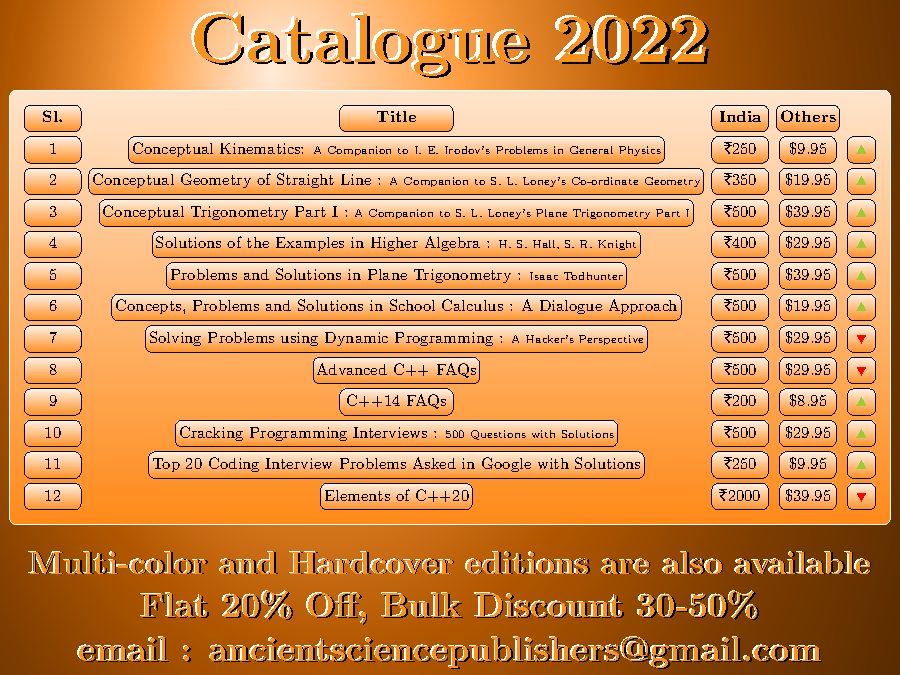
\includegraphics[width=1.0\textwidth]{catalogue/asp-catalogue}
  \end{center}
  %\caption{Front Cover}
%\end{wrapfigure}


\renewcommand{\contentsname}{Monographs}

\pagenumbering{gobble}
\tableofcontents*


\mainmatter

\setlength{\headwidth}{\textwidth}
\setlength{\headwidth}{\textwidth}

\renewcommand{\chaptername}{Monograph}

\part{\textcolor{red}{Computer Science}}

\chapter{Discipline of Competitive Programming : A Hacker’s Perspective}
%\begin{wrapfigure}{r}{0.5\textwidth}
  \begin{center}
    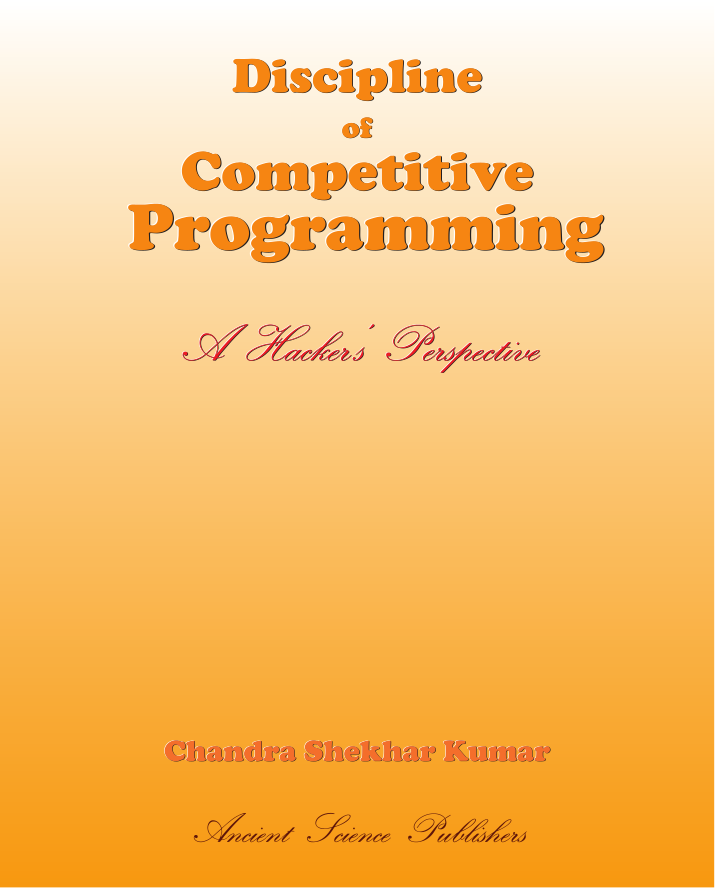
\includegraphics[width=0.8\textwidth]{dcp/cover}
  \end{center}
  %\caption{Front Cover}
%\end{wrapfigure}


\chapter{Elements of Coding : Science of Deriving Correct Programs}
%\begin{wrapfigure}{r}{0.5\textwidth}
  \begin{center}
    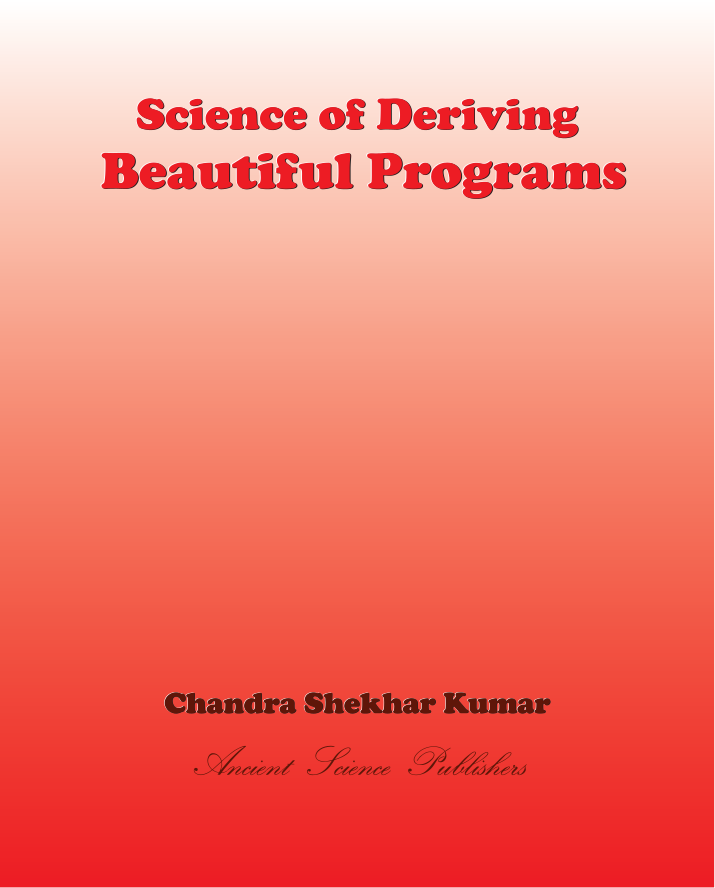
\includegraphics[width=0.8\textwidth]{science-dcp/cover}
  \end{center}
  %\caption{Front Cover}
%\end{wrapfigure}


\chapter{Elements of Coding Linear Algebra : The Nucleus of Artificial Intelligence}
%\chapter{Algebraic Concepts}
%\label{ch1}
%\thispagestyle{empty}
%\protected@edef\concepteq{%
%\[\conceptequiv\]
%}

\underline{\textcolor{BurntOrange}{\textbf{Excerpt from the Chapter \Large \textcolor{Sepia}{Algebraic Concepts}}}}

\vspace{5mm}

\hspace{4mm}\hlt{\textbf{Concept} $\mathcal{C}$ is a predicate describing a set of syntactic and semantic requirements on related types ($<T_i>$) together with a collection of similar procedures $\left(f : T^i \rightarrow T^j\right)$ stated in terms of the properties, attributes and type functions $\left(F : \mathcal{C}^i \rightarrow \mathcal{C}^j \right)$ defined on the types.}
\begin{gather*}
\therefore \mathcal{C}\left(<T_i>\right) \conceptequiv \wedge <\Psi_j>
\end{gather*}
where $\conceptequiv$ stands for \hlt{is defined by} and the $\Psi_j$ represent independent clauses defining the concept.

\begin{lstlisting}
template<class T>
    concept integral = is_integral_v<T>;
\end{lstlisting}

\hlt{If a type $T$ fulfills all the requirements of a concept $\mathcal{C}$, then $T$ \textbf{models} $\mathcal{C}$}, i.e. $T \models \CC$.

\begin{nscenter}
int8\_t and uint8\_t $\models$ \concept{integral}.
\end{nscenter}

\hlt{Concept $\mathcal{C}^i$ is a \textbf{refinement} of concept $\mathcal{C}^j$ if it subsumes the latter, i.e. if $\mathcal{C}^i$ is true for a set of types, then $\mathcal{C}^j$ is also true for the same set.}

In other words, $\mathcal{C}^i$ \hlt{refines} $\mathcal{C}^j$ ($\mathcal{C}^i \refines \mathcal{C}^j$) by addition of more requirements to $\mathcal{C}^j$, i.e. $\mathcal{C}^j$ \hlt{weakens} $\mathcal{C}^i$ ($\mathcal{C}^j \weakens \mathcal{C}^i$). 

\begin{lstlisting}
template<class T>
    concept signed_integral = integral<T> && is_signed_v<T>;
\end{lstlisting}

\begin{nscenter}
\concept{signed\_integral} $\refines$ \concept{integral} \\
int8\_t $\models$ \concept{signed\_integral}  
\end{nscenter}

\begin{lstlisting}
template<class T>
concept unsigned_integral = integral<T> && !signed_integral<T>;
\end{lstlisting}

\begin{nscenter}
\concept{unsigned\_integral} $\refines$ \concept{integral} \\
uint8\_t $\models$ \concept{unsigned\_integral}  
\end{nscenter}




\begin{comment}

{\color{plotptcolor}
\vspace{1in}

\hrule
\vspace{1mm}
\hrule

\fancybreak{$\blacktriangle\blacktriangle\blacktriangle$}
\begin{hindi}
\centering \bfseries\large 
ॐ 
\end{hindi}
\fancybreak{$\blacktriangledown\blacktriangledown\blacktriangledown$}

\hrule
\vspace{1mm}
\hrule}
\end{comment}






\chapter{Elements of Software Design Patterns}
%\begin{center}
\begin{wrapfigure}{r}{0.5\textwidth}
\begin{tikzpicture}[remember picture,overlay]
\begin{scope}[shift={(current page.center)}]
  \node[scale=.6, at={(2.8in, 3.4in)}]
    {\setmainfont{Cooper Black}
\fontsize{2cm}{1.5cm}\selectfont \bfseries {\textcolor{Snow}{\RaisedText{\calligra{Elements}}}}};

\node[scale=.6, at={(2.8in, 2.7in)}]
    {\setmainfont{Cooper Black}
\fontsize{2cm}{1.5cm}\selectfont \bfseries {\textcolor{Snow}{\RaisedText{\calligra{of}}}}};

\node[scale=0.65, at={(3.0in, 2.1in)}]
    {\setmainfont{Cooper Black}
\fontsize{2cm}{1.5cm}\selectfont \bfseries \textcolor{Snow}{\RaisedText{Software Design}}};

\node[scale=0.9, at={(3.0in, 1.3in)}]
    {\setmainfont{Cooper Black}
\fontsize{2cm}{1.5cm}\selectfont \bfseries \textcolor{Snow}{\RaisedText{Patterns}}};


\node[scale=0.4, at={(3in, -2.7in)}]
    {\setmainfont{Cooper Black}
\fontsize{2cm}{1.5cm}\selectfont \bfseries \textcolor{Snow}{\RaisedText{Chandra Shekhar Kumar}}};


\node[scale=0.3, at={(3in, -3.1in)}]
    {\setmainfont{Cooper Black}
\fontsize{2cm}{1.5cm}\selectfont \bfseries \textcolor{Black}{\calligra {Ancient Science Publishers}}};

%design spine 
\node[scale=0.8, rotate=-90,  minimum width=9.3in, minimum height=0.9in,ultra thick] 
at(0,-0.0) 
{
\setmainfont{Cooper Black}
\fontsize{1.0cm}{0.5cm}\selectfont
\begin{varwidth}{17in}
\color{Snow}
\RaisedText{Elements of Software Design Patterns}
\end{varwidth}
};

\begin{scope}[remember picture, xshift=5cm]
\node[ellipse callout, callout pointer shorten=-1.2cm, draw] (hallo) 
{
\begin{varwidth}{1.8in}
I am a pattern.

What are you?
\end{varwidth}
};

\draw[fill=Grey] (-0.5,-4.5) circle [x radius=1.5cm, y radius=5mm];
\draw[fill=Grey] (5,-4.5) circle [x radius=1cm, y radius=5mm];

\begin{scope}[xshift=-3.5cm, yshift=-0.5cm]
\begin{scope}[y=0.80pt, x=0.80pt, yscale=-0.5, xscale=0.5, inner sep=0pt, outer sep=0pt]
\path[draw, fill=Black,even odd rule] (386.4600,182.7600) .. controls (380.5260,182.3640) and (374.0910,184.0390) .. (369.4330,187.7910) .. controls (370.8200,185.4800) and (372.2190,183.4020) .. (373.3020,180.8250) .. controls (366.6320,180.9420) and (360.7610,183.0510) .. (354.6830,185.5840) .. controls (348.1310,188.3130) and (343.0510,182.0710) .. (337.6970,178.5020) .. controls (328.5990,172.4380) and (318.4820,166.3890) .. (313.4880,156.4000) .. controls (308.9610,147.3470) and (301.9760,127.8640) .. (288.2940,129.4720) .. controls (274.2360,131.1270) and (266.4640,123.6190) .. (255.6510,115.8070) .. controls (234.7890,100.7320) and (215.7280,82.8280) .. (188.6990,79.4280) .. controls (161.5340,76.0120) and (135.6750,88.4450) .. (111.4310,98.4280) .. controls (88.7860,107.7520) and (59.5580,119.9360) .. (38.5410,100.3270) .. controls (29.3610,91.7620) and (24.5120,78.5840) .. (21.3670,66.7900) .. controls (17.6240,52.7560) and (24.3950,44.3350) .. (29.9910,32.3460) .. controls (32.4580,27.0580) and (32.3670,-3.2680) .. (21.7070,0.2850) .. controls (12.1280,3.4770) and (12.2530,24.5660) .. (8.6270,32.5420) .. controls (2.6690,45.6470) and (-0.8060,55.1290) .. (0.1620,69.6300) .. controls (0.9820,81.9410) and (6.9130,94.8560) .. (12.9940,105.3670) .. controls (36.1080,145.3280) and (85.7680,142.4600) .. (124.8340,130.1370) .. controls (121.7750,141.9320) and (125.0470,150.5490) .. (127.3430,162.0300) .. controls (128.4310,167.4730) and (128.2430,173.0530) .. (129.0920,178.5120) .. controls (130.1360,185.2330) and (134.1230,190.1210) .. (135.6710,196.3150) .. controls (137.6700,204.3080) and (138.8680,219.8830) .. (134.3170,227.4690) .. controls (127.4420,238.9280) and (134.7940,243.6040) .. (136.0590,254.7530) .. controls (137.2200,264.9820) and (132.6560,275.9590) .. (146.5080,278.3600) .. controls (151.6900,279.2580) and (161.6800,278.2010) .. (164.3100,272.9420) .. controls (168.6440,264.2730) and (161.0060,267.7030) .. (157.5380,264.2340) .. controls (154.8410,261.5390) and (155.0530,252.9090) .. (153.7750,249.0760) .. controls (151.8480,243.2950) and (152.3330,237.9310) .. (154.4420,232.3060) .. controls (158.2770,222.0780) and (166.6630,211.8920) .. (165.0850,200.5710) .. controls (172.1600,211.9720) and (172.4630,221.7580) .. (166.6330,233.8540) .. controls (164.2230,238.8550) and (159.8630,243.8760) .. (161.6020,250.1080) .. controls (162.6430,253.8370) and (165.9040,254.9870) .. (167.7940,257.8480) .. controls (169.8990,261.0370) and (170.7110,264.4470) .. (172.9970,267.4940) .. controls (181.1970,278.4280) and (187.5520,285.7130) .. (202.2380,285.7130) .. controls (208.3370,285.7130) and (212.7340,285.6950) .. (214.2360,278.9410) .. controls (215.8780,271.5520) and (210.7010,270.5280) .. (204.6940,268.9260) .. controls (197.9420,267.1260) and (193.3560,267.9050) .. (190.6280,260.5570) .. controls (188.3880,254.5250) and (189.6850,247.1190) .. (190.5070,240.9530) .. controls (190.9980,237.2670) and (198.1880,229.5340) .. (200.3030,226.1140) .. controls (203.5980,220.7850) and (206.0530,215.3790) .. (209.0320,209.9170) .. controls (217.8900,193.6780) and (226.3260,216.5620) .. (229.9080,226.1140) .. controls (233.9870,236.9900) and (233.4210,253.3020) .. (240.9380,262.1060) .. controls (245.2300,267.1320) and (266.0050,272.2320) .. (265.3190,260.5570) .. controls (264.9940,255.0270) and (254.8840,254.8990) .. (252.5480,251.6560) .. controls (249.7520,247.7760) and (252.5480,239.9970) .. (252.5480,235.4020) .. controls (256.0660,240.3200) and (259.3810,245.7330) .. (263.9000,249.7510) .. controls (268.9880,254.2720) and (269.2890,259.9800) .. (272.6730,265.5890) .. controls (279.3290,276.6240) and (288.1900,281.6540) .. (300.7940,276.0530) .. controls (305.0600,274.1570) and (302.2120,266.1600) .. (299.1820,264.4280) .. controls (292.9670,260.8760) and (290.5570,266.5530) .. (287.3780,259.0100) .. controls (283.2070,249.1100) and (283.6690,235.3660) .. (282.1530,224.7590) .. controls (281.6320,221.1110) and (292.9140,225.4690) .. (296.0860,225.6670) .. controls (301.0350,225.9760) and (309.7770,223.9760) .. (314.0810,225.3410) .. controls (318.7460,226.8200) and (321.0190,233.0080) .. (324.5310,236.1760) .. controls (329.6070,240.7570) and (335.3810,244.3040) .. (342.3760,244.3040) .. controls (353.9930,244.3040) and (358.2910,259.8880) .. (372.5200,254.7530) .. controls (375.6520,253.6230) and (382.3360,250.9170) .. (382.7760,247.4000) .. controls (383.5000,241.6150) and (378.4720,237.9130) .. (379.8740,232.3060) .. controls (381.9430,224.0280) and (378.0000,215.0970) .. (375.6170,207.1510) .. controls (373.7900,201.0560) and (372.8770,198.9840) .. (377.3590,193.6040) .. controls (380.2590,190.1440) and (383.1690,185.8940) .. (386.4590,182.7940);




\path[draw=black,fill=Snow,even odd rule,line width=0.249pt,miter limit=5.33] (374.8400,224.5600) .. controls (370.1790,224.1080) and (362.2460,225.3020) .. (365.5520,231.9140) .. controls (369.9820,240.7540) and (373.5020,228.1540) .. (374.8420,224.5640);



\path[draw=black,line cap=rect,line width=0.249pt,miter limit=5.33] (382.5800,245.8400) .. controls (385.0340,240.3050) and (389.2710,235.2550) .. (394.5780,232.2960);



\path[draw=black,line cap=rect,line width=0.249pt,miter limit=5.33] (376.0000,248.9400) .. controls (365.0840,249.4720) and (356.6660,254.6200) .. (348.9100,262.0980);



\path[draw=black,line cap=rect,line width=0.249pt,miter limit=5.33] (367.8800,245.8400) .. controls (359.2980,247.8990) and (350.4040,248.1800) .. (341.9500,250.4850);



\path[draw=black,line cap=rect,line width=0.249pt,miter limit=5.33] (360.9100,250.1000) .. controls (352.0790,251.4510) and (343.5320,253.4170) .. (335.3680,257.0670);



\path[draw=black,fill=Black,even odd rule,line width=0.249pt,miter limit=5.33] (382.9700,244.3000) .. controls (379.9050,245.1640) and (379.0350,248.1570) .. (376.0040,248.9450) .. controls (378.8140,253.6450) and (383.9040,249.0350) .. (382.9740,244.3050);



\path[draw=black,fill=Black,even odd rule,line width=0.249pt,miter limit=5.33] (370.9700,224.9500) .. controls (371.4990,228.0060) and (370.8810,231.0770) .. (368.6490,233.0770) .. controls (369.1990,229.9370) and (368.8390,225.8270) .. (370.9690,224.9470);
\end{scope}
\end{scope}
\begin{scope}[xshift=5cm]
\node[ellipse callout, callout relative pointer={(0,-1)}, draw] (hallo) 
{
\begin{varwidth}{1.5in}
Quality \\without \\ a name!
%\texthindi{मैं बहुरुपिया कोरोना।}
\end{varwidth}
};
\end{scope}
\end{scope}
\end{scope}
\end{tikzpicture}
%\end{center}
\end{wrapfigure}

\underline{\textbf{\textcolor{BurntOrange}{Excerpt from the Chapter} \textcolor{Sepia}{(Pattern Concept):}}}

\begin{defn}
A pattern is a rule triad expressing a relation between:
\begin{enumerate}
  \item a certain \hlt{context} defining the scope of applicability of the given pattern,
  \item a \hlt{problem} detailing a certain system of conflicting forces which occurs repeatedly that the pattern resolves in that context and
  \item a \hlt{solution} in a form of a certain software configuration which can be used repeatedly and uniquely to resolve the given system of forces themselves, wherever the context makes it relevant.
\end{enumerate}
\par\vspace{-1.8\baselineskip}
\qedhere
\end{defn}

%\begin{warpHTML}
\begin{wrapfigure}{l}{0.5\textwidth}
  \begin{center}
    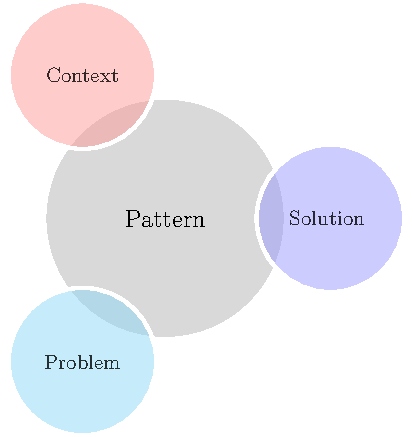
\includegraphics[width=0.5\textwidth]{designpatterns/patterns-triad}
  \end{center}
  %\caption{Front Cover}
\end{wrapfigure}
%\end{warpHTML}


The output of this rule triad is a pattern too.

\vspace{4mm}

It leads (but not limited) to the following  key observations about pattern:
%\begin{enumerate}[label=\protect\circnode{\color{red}\arabic*}]
\begin{dinglist}{213}
\item It is both a thing and a process.
\item It is both a description of a thing which is alive and a description of the process which will generate that thing.
\item It is both a thing which happens in the world and the rule which tells us how to create that thing.
\item It can exist at all scales and resolve almost any kind of conflicting forces.
\item Identification of what-why-when-where marks its inner structure explicit and sharable.
\item It starts with defining features worth abstracting.
\item Then it defines the problem, i.e. the field of forces which it brings into balance.
\item It is a sketch rather than a blue-print. 
\item It can complement and compound another pattern(s).
\item It is generative and self-sustaining.
\item It is a micro-architecture.
\item It promotes design-reuse.
\item The exact range of contexts is defined where the stated problem occurs and where this particular solution to the problem is appropriate.
\item Each pattern describes a problem which occurs over and over again in our system and then describes the core of the solution to that problem in such a way that we can use this solution a million times over, without ever doing it the same way twice.
\end{dinglist}

Beyond its elements, each system is defined by a certain patterns of relationships among the elements, and these relationships are integral part of the elements to such an extent that the elements themselves are patterns of relationships. And finally, the so called elements get dissolved, leaving patterns of relationships behind, which is the actual thing that actually repeats itself and gives structure to the system.

Each one of these patterns $\mathcal{P}_i$  is a morphological law onto itself, which establishes a set of relationships in the system in a given context of type $\mathcal{C}$, i.e.
\hlm{\begin{gather*}
\mathcal{P}_i \triangleq \mathcal{C} \rightarrow \mathcal{R}\left(\ldots, \mathcal{P}_{i-1}, \mathcal{P}_{i+1}, \ldots\right)
\end{gather*}} 
where $\triangleq$ stands for \hlt{is defined by}. The parts (i.e, rest of the patterns except $\mathcal{P}_i$) $\ldots, \mathcal{P}_{i-1}, \mathcal{P}_{i+1}, \ldots$ are related by the relationship $\mathcal{R}$ within a context of type $\mathcal{C}$.

Note that, each law or pattern is itself a pattern of relationships among the remaining laws (i.e. except itself), which are themselves just patterns of relationships again.

\hlt{Therefore, a pattern is defined by formulating it in the form of a rule triad as depicted before,  which establishes a relationship between a context, a system of (often conflicting) forces which arise in that context and configuration which allows these forces to resolve themselves in that context.}

\vspace{3mm}

Hence, generic form of each pattern is:

%\begin{wrapfigure}{r}{0.5\textwidth}
  \begin{center}
    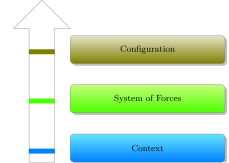
\includegraphics[width=0.7\textwidth]{designpatterns/patterns-form}
  \end{center}
  %\caption{Front Cover}
%\end{wrapfigure}

Discovery of (the invariant features) pattern(s) always start with observation or purely abstract argument. This process is not sequential from the problem to the solution or vice versa. Rather it is a multidimensional global process to help identify a solid and reliable invariant which relates context, problem, solution in an unchanging way. 

The statement of the problem and the forces helps to solidify the pattern which is responsible for making the system of forces come to an equilibrium. Thought it is still tentative, but clear enough to be shared.

There are two components in a pattern definition, which are empirical in nature, i.e. can be tested as true/false:
\begin{enumerate}
\item The problem is real, i.e. it is expressible as conflicting real forces within the stated context(s).
\item The configuration solves the problem, i.e. it deals with all the forces in the stated context(s).
\end{enumerate}
Quality without a name is the living essence of a pattern.

\vspace{20mm}

\underline{\textbf{\textcolor{BurntOrange}{Excerpt from the Chapter} \textcolor{Sepia}{(Pattern Form):}}}

\hspace{5mm}Each (living) pattern has the same form for the sake of convenience and clarity. It has \hlt{nine} parts in the following sequence :
\begin{enumerate}[label=\protect\circnode{\color{Sepia}\arabic*}]
\item A \hlt{picture} is drawn to illustrate an archetypal example of the pattern.
\item An \hlt{introductory paragraph} to set the context for the pattern.
\item The symbol \hl{\texthindi{ॐ}} marks the beginning of the problem the pattern addresses later.
\item A \hlbt{headline} set in bold-typeface to provide the essence of the problem.
\item The \hlt{body} of the problem describing (but not limited to) the 
    \begin{dinglist}{213}
        \item empirical background of the pattern,
        \item empirical evidence for its validity which sets the motivational tone too,
        \item variations, i.e. the range of different ways of manifesting it in a software.
    \end{dinglist}
\item The \hlbt{solution} set in bold-typeface, encoded in an instructional form, stating the exact steps to build the pattern. It illustrates the field of relationships needed to solve the stated problem in the stated context.
\item A \hlt{diagram} that shows the solution as a labeled picture indicating its main components.
\item The symbol \hl{\texthindi{ॐ}} marking the end of the main body of the pattern.
\item A \hlt{paragraph}, which ties the pattern to all those smaller patterns in the pattern language, which are needed to complete this pattern, to embellish it, to fill it out.
\end{enumerate}

This form serves the following two essential purposes :
\begin{enumerate}[itemsep=0.3em]%[label=\protect\circnode{\color{Sepia}\arabic*}]
    \item to present each pattern connected to other patterns to help grasp the collection of all these patterns as a whole, as a pattern language, within which an infinite variety of combinations can be created.
    \item to present the problem and solution of each pattern in such a way that it sets the exact tone of self-judgment and modifications without losing the central essence. 
\end{enumerate}

\vspace{20mm}

\underline{\textbf{\textcolor{BurntOrange}{Excerpt from the Chapter} \textcolor{Sepia}{(Null Object):}}}

\epigraphhead[30]
{
\epigraph{\hlt{Do what you can to establish coherence in your software. I am smart because I do nothing!}}{}

}

\begin{center}
\begin{tikzpicture}[remember picture]
\node[ellipse callout, callout pointer shorten=-1.2cm, draw] (hallo) 
{
\begin{varwidth}{1.5in}
I am a reference!

What are you?
%\begin{hindi}
%मैं वैक्सीन हूँ। 

%तू कौन है?
%\end{hindi}
\end{varwidth}
};

\draw[fill=Grey] (-0.5,-4) circle [x radius=1.5cm, y radius=5mm];
\draw[fill=Grey] (5,-4) circle [x radius=1cm, y radius=5mm];

\begin{scope}[xshift=-3.5cm]
\begin{scope}[y=0.80pt, x=0.80pt, yscale=-0.5, xscale=0.5, inner sep=0pt, outer sep=0pt]
\path[draw, fill=Orange,even odd rule] (386.4600,182.7600) .. controls (380.5260,182.3640) and (374.0910,184.0390) .. (369.4330,187.7910) .. controls (370.8200,185.4800) and (372.2190,183.4020) .. (373.3020,180.8250) .. controls (366.6320,180.9420) and (360.7610,183.0510) .. (354.6830,185.5840) .. controls (348.1310,188.3130) and (343.0510,182.0710) .. (337.6970,178.5020) .. controls (328.5990,172.4380) and (318.4820,166.3890) .. (313.4880,156.4000) .. controls (308.9610,147.3470) and (301.9760,127.8640) .. (288.2940,129.4720) .. controls (274.2360,131.1270) and (266.4640,123.6190) .. (255.6510,115.8070) .. controls (234.7890,100.7320) and (215.7280,82.8280) .. (188.6990,79.4280) .. controls (161.5340,76.0120) and (135.6750,88.4450) .. (111.4310,98.4280) .. controls (88.7860,107.7520) and (59.5580,119.9360) .. (38.5410,100.3270) .. controls (29.3610,91.7620) and (24.5120,78.5840) .. (21.3670,66.7900) .. controls (17.6240,52.7560) and (24.3950,44.3350) .. (29.9910,32.3460) .. controls (32.4580,27.0580) and (32.3670,-3.2680) .. (21.7070,0.2850) .. controls (12.1280,3.4770) and (12.2530,24.5660) .. (8.6270,32.5420) .. controls (2.6690,45.6470) and (-0.8060,55.1290) .. (0.1620,69.6300) .. controls (0.9820,81.9410) and (6.9130,94.8560) .. (12.9940,105.3670) .. controls (36.1080,145.3280) and (85.7680,142.4600) .. (124.8340,130.1370) .. controls (121.7750,141.9320) and (125.0470,150.5490) .. (127.3430,162.0300) .. controls (128.4310,167.4730) and (128.2430,173.0530) .. (129.0920,178.5120) .. controls (130.1360,185.2330) and (134.1230,190.1210) .. (135.6710,196.3150) .. controls (137.6700,204.3080) and (138.8680,219.8830) .. (134.3170,227.4690) .. controls (127.4420,238.9280) and (134.7940,243.6040) .. (136.0590,254.7530) .. controls (137.2200,264.9820) and (132.6560,275.9590) .. (146.5080,278.3600) .. controls (151.6900,279.2580) and (161.6800,278.2010) .. (164.3100,272.9420) .. controls (168.6440,264.2730) and (161.0060,267.7030) .. (157.5380,264.2340) .. controls (154.8410,261.5390) and (155.0530,252.9090) .. (153.7750,249.0760) .. controls (151.8480,243.2950) and (152.3330,237.9310) .. (154.4420,232.3060) .. controls (158.2770,222.0780) and (166.6630,211.8920) .. (165.0850,200.5710) .. controls (172.1600,211.9720) and (172.4630,221.7580) .. (166.6330,233.8540) .. controls (164.2230,238.8550) and (159.8630,243.8760) .. (161.6020,250.1080) .. controls (162.6430,253.8370) and (165.9040,254.9870) .. (167.7940,257.8480) .. controls (169.8990,261.0370) and (170.7110,264.4470) .. (172.9970,267.4940) .. controls (181.1970,278.4280) and (187.5520,285.7130) .. (202.2380,285.7130) .. controls (208.3370,285.7130) and (212.7340,285.6950) .. (214.2360,278.9410) .. controls (215.8780,271.5520) and (210.7010,270.5280) .. (204.6940,268.9260) .. controls (197.9420,267.1260) and (193.3560,267.9050) .. (190.6280,260.5570) .. controls (188.3880,254.5250) and (189.6850,247.1190) .. (190.5070,240.9530) .. controls (190.9980,237.2670) and (198.1880,229.5340) .. (200.3030,226.1140) .. controls (203.5980,220.7850) and (206.0530,215.3790) .. (209.0320,209.9170) .. controls (217.8900,193.6780) and (226.3260,216.5620) .. (229.9080,226.1140) .. controls (233.9870,236.9900) and (233.4210,253.3020) .. (240.9380,262.1060) .. controls (245.2300,267.1320) and (266.0050,272.2320) .. (265.3190,260.5570) .. controls (264.9940,255.0270) and (254.8840,254.8990) .. (252.5480,251.6560) .. controls (249.7520,247.7760) and (252.5480,239.9970) .. (252.5480,235.4020) .. controls (256.0660,240.3200) and (259.3810,245.7330) .. (263.9000,249.7510) .. controls (268.9880,254.2720) and (269.2890,259.9800) .. (272.6730,265.5890) .. controls (279.3290,276.6240) and (288.1900,281.6540) .. (300.7940,276.0530) .. controls (305.0600,274.1570) and (302.2120,266.1600) .. (299.1820,264.4280) .. controls (292.9670,260.8760) and (290.5570,266.5530) .. (287.3780,259.0100) .. controls (283.2070,249.1100) and (283.6690,235.3660) .. (282.1530,224.7590) .. controls (281.6320,221.1110) and (292.9140,225.4690) .. (296.0860,225.6670) .. controls (301.0350,225.9760) and (309.7770,223.9760) .. (314.0810,225.3410) .. controls (318.7460,226.8200) and (321.0190,233.0080) .. (324.5310,236.1760) .. controls (329.6070,240.7570) and (335.3810,244.3040) .. (342.3760,244.3040) .. controls (353.9930,244.3040) and (358.2910,259.8880) .. (372.5200,254.7530) .. controls (375.6520,253.6230) and (382.3360,250.9170) .. (382.7760,247.4000) .. controls (383.5000,241.6150) and (378.4720,237.9130) .. (379.8740,232.3060) .. controls (381.9430,224.0280) and (378.0000,215.0970) .. (375.6170,207.1510) .. controls (373.7900,201.0560) and (372.8770,198.9840) .. (377.3590,193.6040) .. controls (380.2590,190.1440) and (383.1690,185.8940) .. (386.4590,182.7940);




\path[draw=black,fill=Snow,even odd rule,line width=0.249pt,miter limit=5.33] (374.8400,224.5600) .. controls (370.1790,224.1080) and (362.2460,225.3020) .. (365.5520,231.9140) .. controls (369.9820,240.7540) and (373.5020,228.1540) .. (374.8420,224.5640);



\path[draw=black,line cap=rect,line width=0.249pt,miter limit=5.33] (382.5800,245.8400) .. controls (385.0340,240.3050) and (389.2710,235.2550) .. (394.5780,232.2960);



\path[draw=black,line cap=rect,line width=0.249pt,miter limit=5.33] (376.0000,248.9400) .. controls (365.0840,249.4720) and (356.6660,254.6200) .. (348.9100,262.0980);



\path[draw=black,line cap=rect,line width=0.249pt,miter limit=5.33] (367.8800,245.8400) .. controls (359.2980,247.8990) and (350.4040,248.1800) .. (341.9500,250.4850);



\path[draw=black,line cap=rect,line width=0.249pt,miter limit=5.33] (360.9100,250.1000) .. controls (352.0790,251.4510) and (343.5320,253.4170) .. (335.3680,257.0670);



\path[draw=black,fill=Black,even odd rule,line width=0.249pt,miter limit=5.33] (382.9700,244.3000) .. controls (379.9050,245.1640) and (379.0350,248.1570) .. (376.0040,248.9450) .. controls (378.8140,253.6450) and (383.9040,249.0350) .. (382.9740,244.3050);



\path[draw=black,fill=Black,even odd rule,line width=0.249pt,miter limit=5.33] (370.9700,224.9500) .. controls (371.4990,228.0060) and (370.8810,231.0770) .. (368.6490,233.0770) .. controls (369.1990,229.9370) and (368.8390,225.8270) .. (370.9690,224.9470);
\end{scope}
\end{scope}

\begin{scope}[xshift=5cm]
\node[ellipse callout, callout relative pointer={(0,-1)}, draw] (hallo) 
{
\begin{varwidth}{1.5in}
I am a null \\reference!
%\texthindi{मैं बहुरुपिया कोरोना।}
\end{varwidth}
};
\end{scope}

%\node at (-3,0.3) {\tiny \copyright \texthindi{शेखर}};
\end{tikzpicture}
\end{center}

%\thispagestyle{empty}

\vspace{3mm}

$\cdots$ consider now the character of settlements within the object references : what balance of real objects and null references is in keeping with the transparency ?

\begin{center}
\hl{\aum} 
\end{center}

\begin{quote}
\hspace{5mm}\hlbt{Optionally null object references, where the result of a null check is to do nothing, will not come to balance until both the presence of a null reference and the absence of an object be treated in a consistent and transparent manner to establish an independent and coherent sphere of object references.}
\end{quote}

\vspace{3mm}

Out of a list of objects, some may not exist. Hence no service is expected in such cases which can be an acceptable behavior too. Acceptable inaction is represented at times with repetitive explicit checking for the optional null. Repetition and optional doesn't go together. Absence of objects can be abstracted out to presence of objects doing nothing, i.e. conformance to the interface with no implied functionality. No-op is the correct operation. We need a way to represent the object with appropriate behavior that will allow us to treat all object references in a consistent and uniform way, devoid of special case consideration.

Typical scenarios under consideration are
\begin{enumerate}[topsep=0em, itemsep=0.2em]
\item Some object instances are not required to do anything because they correspond to null references.
\item These instances should be treated in the same manner as real instances to avoid explicit constraints.
\item There is a need to reuse the do nothing behavior to enforce consistent and repetitive usage.
\end{enumerate}

\hlt{Null Object} patterns addresses all of these under a single umbrella, typically by encapsulating the do nothingness.








\chapter{Elements of Coding AI}

\chapter{Elements of Coding DL (Deep Learning)}

\chapter{Elements of Coding ML : Internals of Machine Learning Library MLPack}

\chapter{Conceptual BitCoin : Blockchain Coding}

\chapter{Conceptual Data Science Interviews}

\chapter{Conceptual Dependency Injection : Unwiring Simplified in C++}

\chapter{Conceptual Dynamic Programming : Optimal Coding Simplified}

\chapter{Conceptual Programming Interviews}

\chapter{Conceptual Machine Learning}

\chapter{Conceptual Programming of STL Algorithms}

\chapter{Conceptual Solutions to (CLRS) Introduction to Algorithms}

\chapter{Conceptual Programming of Algorithms Using Dijkstra’s Approach}

\chapter{Conceptual Solutions to Pattern Recognition and Machine Learning}

\chapter{Science of Deriving Beautiful Programs}

\chapter{Modern C++ Ranges : A Revolution in STL}

\chapter{Elements of C++20}

\begin{wrapfigure}{r}{0.5\textwidth}
  \begin{center}
    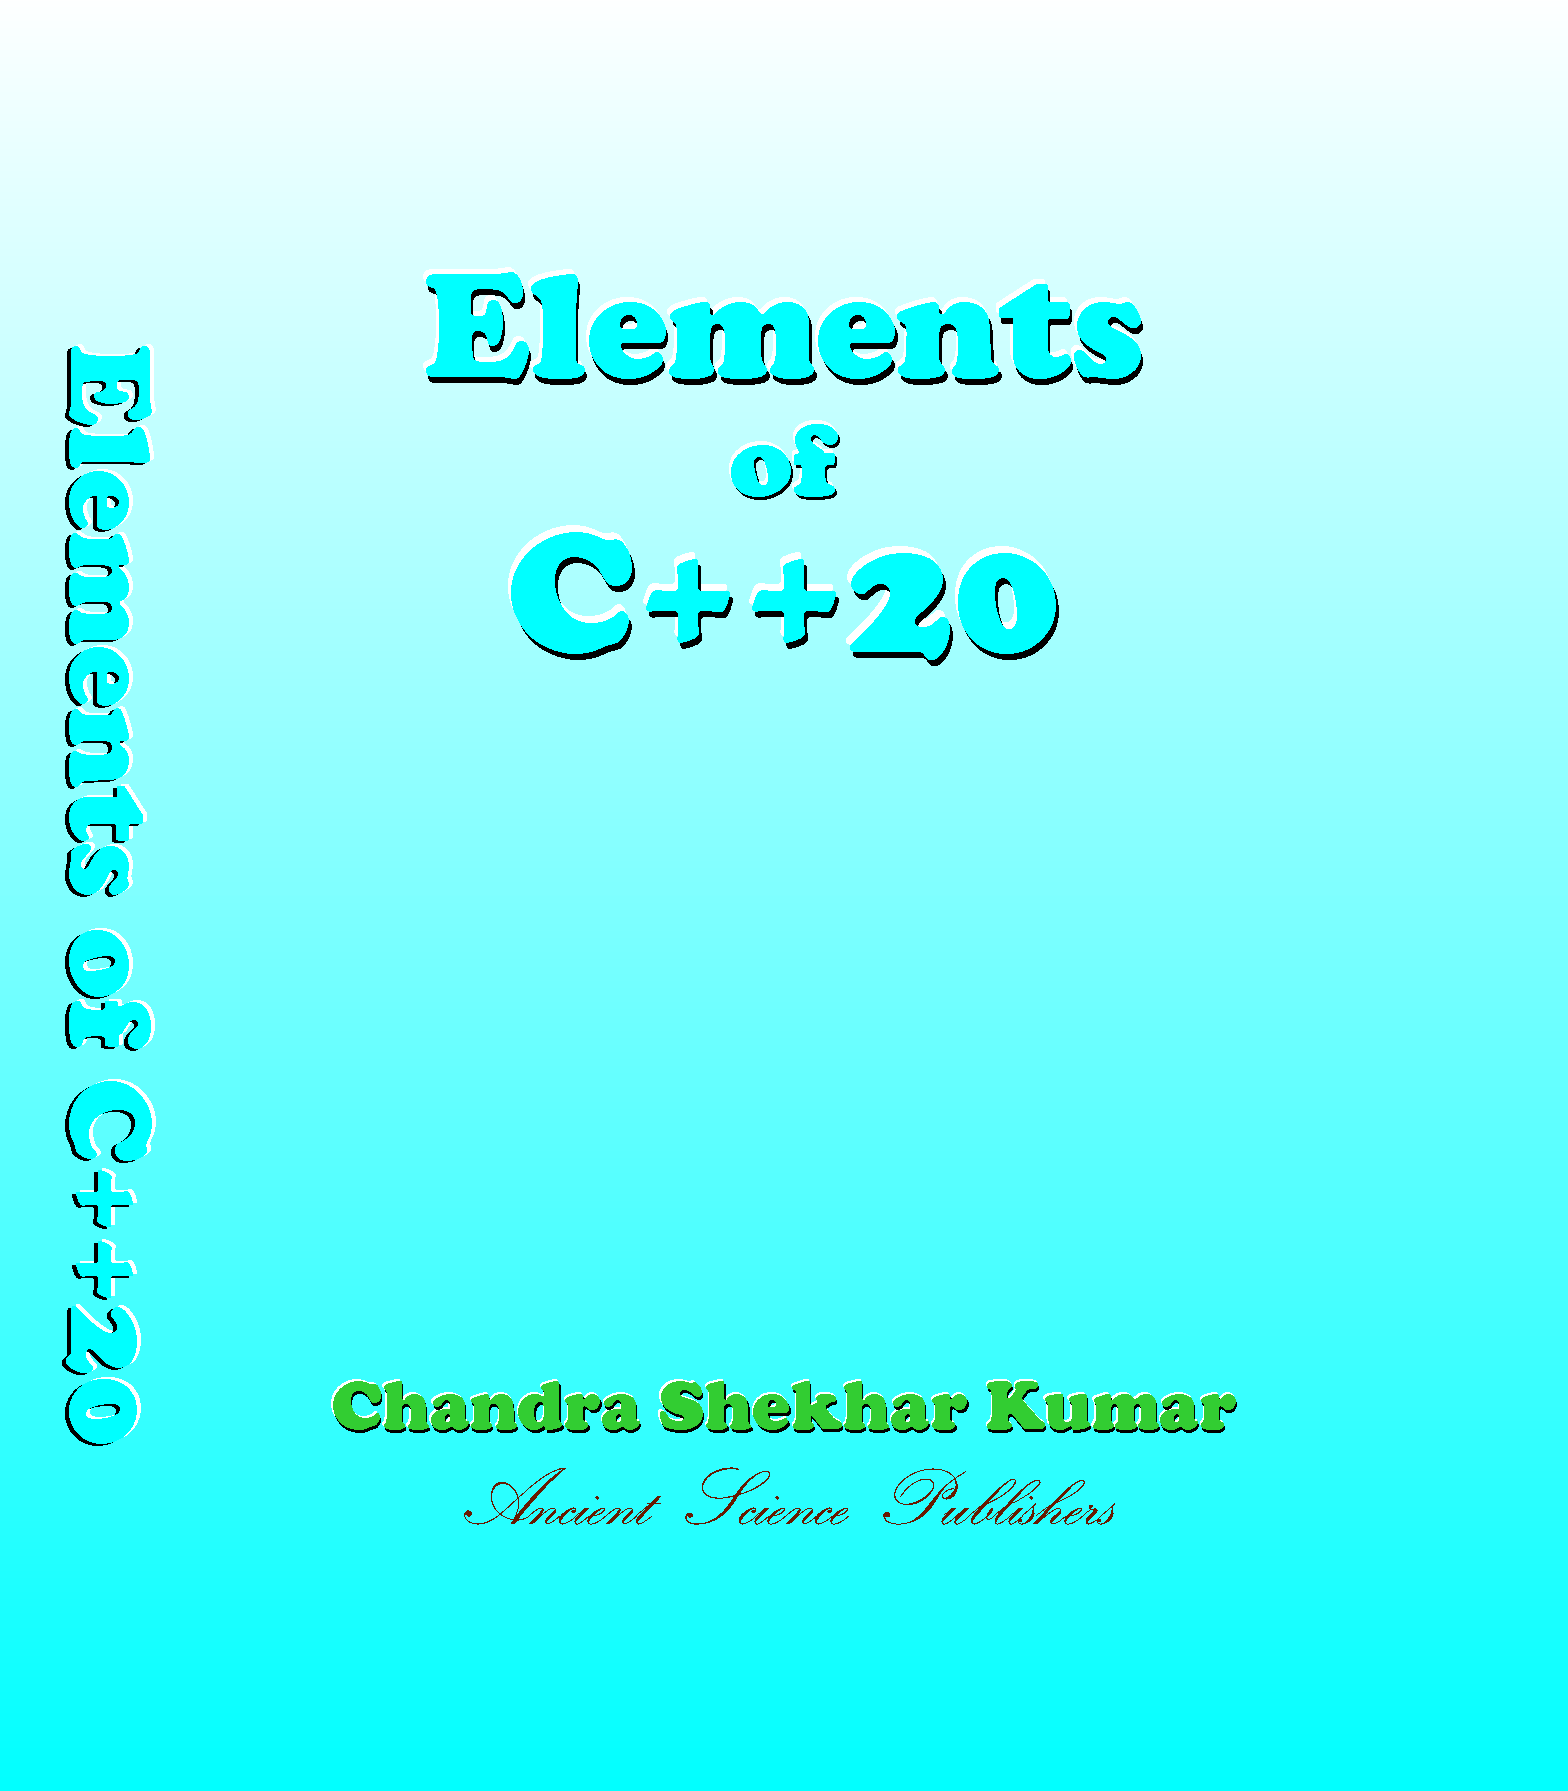
\includegraphics[width=0.5\textwidth]{cpp20/cover}
  \end{center}
  %\caption{Front Cover}
\end{wrapfigure}

\hspace{5mm}This book is a rigorous treatment of salient features of C++ 20 language and library in line with ISO/IEC standard to suit the needs of practicing professionals and experts alike. Armed with \textbf{2000+} examples and 1000+ indices with emphasis on standard library with indicative approach to implementation, it stands as a quick reference too for important concepts. 

\vspace{2mm}

I am grateful for this opportunity to put the materials into a consistent format, and to correct errors in the original ISO/IEC draft that have come to my attention. The process of compiling this book has given me an incentive to improve and extend the text, concepts, problems, solutions, layout, to double check almost all of the mathematical rendering, to correct all known errors, to improve the original illustrations by redrawing them with Till Tantau's marvellous \textup{Ti\textit{k}Z}, to include new diagrams. Thus the book now appears in a form that I hope will remain useful for at least another decade.

\section{Table of Contents}
\setlist{nosep}
\begin{enumerate}%[label*=\arabic*.]
\item Modules
    \begin{enumerate}[label=\arabic{enumi}.\arabic*., itemindent=!]
      \item Module units and purviews
      \item Export declaration 
      \item Import declaration 
      \item Global module fragment 
      \item Private module fragment 
      \item Instantiation context 
      \item Reachability
    \end{enumerate}
\item Classes
    \begin{enumerate}[label=\arabic{enumi}.\arabic*., leftmargin=*]
      \item Preamble   
      \item Properties of classes 
      \item Class names 
      \item Class members 
      \item Unions 
      \item Local class declarations
      \item Derived classes 
      \item Member access control 
      \item Initialization 
      \item Comparisons 
      \item Free store
    \end{enumerate}
\item Overloading
    \begin{enumerate}[label=\arabic{enumi}.\arabic*., leftmargin=*]
      \item Preamble 
      \item Overload resolution 
      \item Address of an overload set
      \item Overloaded operators 
      \item Built-in operators 
      \item User-defined literals
    \end{enumerate}
\item Templates
    \begin{enumerate}[label=\arabic{enumi}.\arabic*.]
      \item Preamble 
      \item Template parameters 
      \item Names of template specializations 
      \item Template arguments 
      \item Template constraints 
      \item Type equivalence 
      \item Template declarations
      \item Name resolution 
      \item Template instantiation and specialization
      \item Function template specializations
    \end{enumerate}
\item Exception handling
    \begin{enumerate}[label=\arabic{enumi}.\arabic*.]
      \item Preamble 
      \item Throwing an exception 
      \item Constructors and destructors
      \item Handling an exception 
      \item Exception specifications 
      \item Special functions
     \end{enumerate}
\item Concepts library
    \begin{enumerate}[label=\arabic{enumi}.\arabic*.]
      \item General 
      \item Equality preservation 
      \item Header <concepts> synopsis 
      \item Language-related concepts 
      \item Comparison concepts 
      \item Object concepts 
      \item Callable concepts
     \end{enumerate}
\item General utilities library
    \begin{enumerate}[label=\arabic{enumi}.\arabic*.]
      \item General 
      \item Utility components 
      \item Compile-time integer sequences 
      \item Pairs 
      \item Tuples 
      \item Optional objects  
      \item Variants 
      \item Storage for any type 
      \item Bitsets 
      \item Memory 
      \item Smart pointers 
      \item Memory resources 
      \item Class template scoped\_allocator\_adaptor
      \item Function objects
      \item Metaprogramming and type traits 
      \item Compile-time rational arithmetic 
      \item Class type\_index 
      \item Execution policies 
      \item Primitive numeric conversions 
      \item Formatting 
      \item Stacktrace
     \end{enumerate}
\item Strings library
    \begin{enumerate}[label=\arabic{enumi}.\arabic*.]
      \item General 
      \item Character traits 
      \item String classes
      \item String view classes
      \item Null-terminated sequence utilities
     \end{enumerate}
\item Containers library
    \begin{enumerate}[label=\arabic{enumi}.\arabic*.]
      \item General 
      \item Container requirements
      \item Sequence containers 
      \item Associative containers 
      \item Unordered associative containers
      \item Container adaptors 
      \item Views
     \end{enumerate}
\item Iterators library
    \begin{enumerate}[label=\arabic{enumi}.\arabic*.]
      \item General 
      \item Header <iterator> synopsis
      \item Iterator requirements 
      \item Iterator primitives 
      \item  Iterator adaptors 
      \item Stream iterators 
      \item  Range access
     \end{enumerate}
\item Ranges library
    \begin{enumerate}[label=\arabic{enumi}.\arabic*.]
      \item General       
      \item Header <ranges> synopsis
      \item Range access 
      \item Range requirements 
      \item Range utilities 
      \item Range factories 
      \item Range adaptors
     \end{enumerate}
\item Algorithms library
    \begin{enumerate}[label=\arabic{enumi}.\arabic*.]
      \item  General 
      \item  Algorithms requirements 
      \item Parallel algorithms 
      \item Header <algorithm> synopsis 
      \item Algorithm result types 
      \item Non-modifying sequence operations
      \item  Mutating sequence operations 
      \item Sorting and related operations 
      \item Header <numeric> synopsis 
      \item Generalized numeric operations 
      \item Specialized <memory> algorithms 
      \item C library algorithms
     \end{enumerate}
\end{enumerate}      
      
      
      
      
      
      
      

\chapter{Solving Problems using Dynamic Programming : A Hacker’s Perspective}

\begin{warpHTML}
\begin{wrapfigure}{r}{0.5\textwidth}
  \begin{center}
    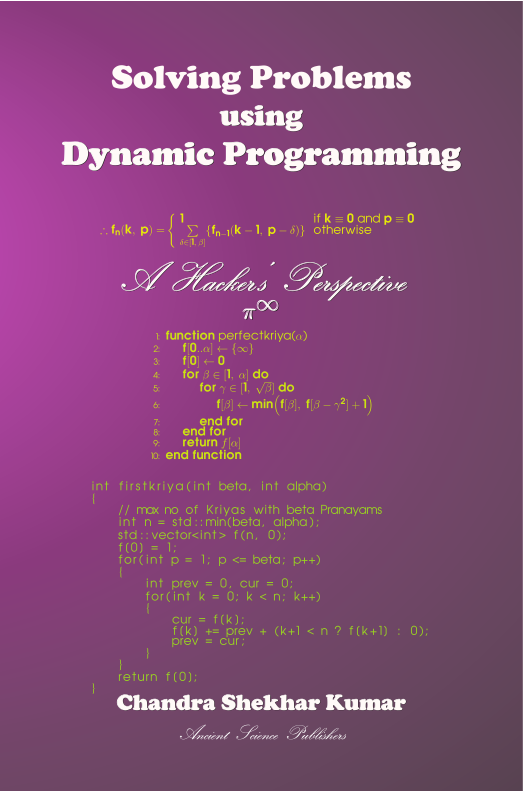
\includegraphics[width=0.5\textwidth]{solvingdpp/cover/dpp-cover}
  \end{center}
  %\caption{Front Cover}
\end{wrapfigure}
\end{warpHTML}

\hspace{5mm}A hacker's approach to a coding problem is beyond the foundational aspect of underlying genetic and computational structures, often termed as $\color{Orange}\mathbf{\pi^\infty}$.  

\begin{warpprint}
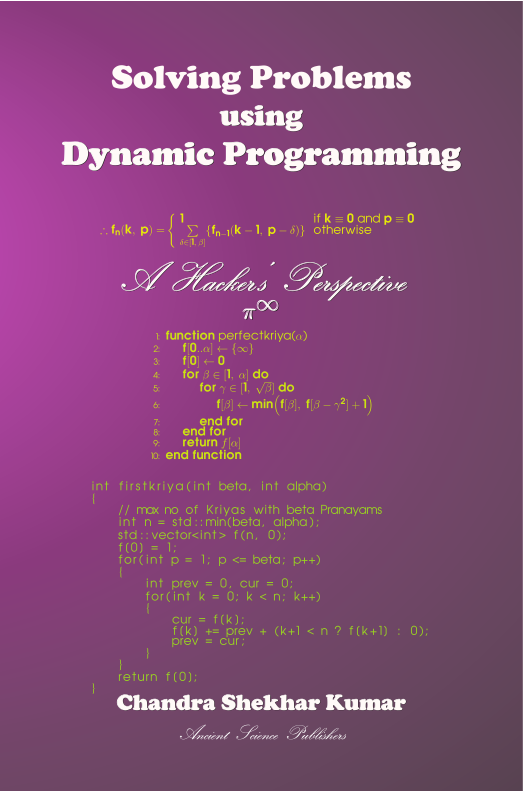
\includegraphics[width=0.5\linewidth]{solvingdpp/cover/dpp-cover}
\end{warpprint}

\hspace{5mm}A concept becomes \hlt{not difficult} because the \hlt{complexities} built into it are clarified. In a bid to reach the \hlt{core} of the problem, the concept is split-broken into fragments,  \hlt{complexities} are exposed and \hlt{delicate} points are examined. Then the concept is \hlt{recomposed} to make it integral and as a result, this reintegrated concept becomes sufficiently simple and comprehensible. 

\hspace{5mm}This helps build a hacker's insight to reveal the internal structure and internal logic of the concepts, algorithms and mathematical theorems.

\vspace{3mm}

This book provides a hacker's perspective to solving problems using dynamic programming. Written in an extremely lively form of problems and solutions (including code in modern C++ and pseudo style), this leads to extreme simplification of optimal coding with great emphasis on unconventional and integrated science of dynamic Programming. Though aimed primarily at serious programmers, it imparts the knowledge of deep internals of underlying concepts and beyond to computer scientists alike.


\vspace{0.2in}

\noindent {\calligra Ancient Science Publishers}  \hfill \emph{Chandra Shekhar Kumar}

\noindent July, 2020. \hfill 256 pages \hfill ISBN  9781722497170

\vspace{5mm}

\begin{quote}
\hspace{5mm}\hlt{Beautiful (C++) code snippets. Unique yogic exposition to coding.}
\end{quote}
\hfill {\calligra Ancient Science Hackers}


\vspace{10mm}


\underline{\textbf{\textcolor{BurntOrange}{Excerpt from the Chapter} \textcolor{Sepia}{(Optimal Loot Partition):}}}


\begin{p}
\hlt{The head of a gang of robbers embarks on distribution of the looted amount $l (> 0)$, starting with division into two parts : $x$ and $l - x$ for $0 \le x \le l$. From $x$ : they get a return of $u(x)$ such that they are left with a lesser amount $\alpha x$ : $0 < \alpha < 1$ and from $l - x$ : a return of $v(l - x)$ such that they are left with a lesser amount $\beta(l - x)$ : $0 < \beta < 1$. So the total amount left after the first step of division is $\alpha x + \beta (l - x)$ and the process continues. Devise the partition strategy to help them maximize the return obtained in a finite $n$ or infinite number of steps.}
\end{p}

\begin{s}
Let $y(x)$ denote the return after the first step:
\begin{gather*}
\therefore y(x) = u(x) + v(l - x)
\end{gather*}
Assuming $u$ and $v$ to be continuous functions, it is trivial to find the maximum of $y(x)$ over $x \in [0, l]$ using calculus (or graphical approach) :
\begin{gather*}
\dfrac{d y}{d x} = \dfrac{d}{d x} u(x) + \dfrac{d}{d x} v(l - x) = 0 \text{ (for extrema)}.
\end{gather*}
Solve for $x$ and $y(x)$ is maximum for that $x$ for which $\dfrac{d^2 y}{d x^2} < 0$.

Suppose $u(x) = x$ and $v(l - x) = -(l - x)^2 $, then 
\begin{gather*}
y = x - (l - x)^2 \\
\therefore \dfrac{d y}{d x} = 1 + 2(l - x) = 0, \\
\therefore x = l + \dfrac{1}{2}.\\
\dfrac{d^2 y}{d x^2} = -2 < 0. \\
\therefore y_{max} = l + \dfrac{1}{2} - \dfrac{1}{4} = l + \dfrac{1}{4}. 
\end{gather*}
After the first step, the initial amount $l$ is reduced to $l_1$(say):
\begin{gather*}
\therefore l_1 = \alpha x + \beta (l - x) 
\end{gather*}
In the second step, $l_1$ is partitioned into $x_1$ (say) and $(l_1 - x_1)$ for $0 \le x_1 \le l_1$. Hence, the return from the second step is $u(x_1) + v(l_1 - x_1)$. Therefore, the total return after the two steps is:
\begin{gather*}
\therefore y(x, x_1) = u(x) + v(l - x) + u(x_1) + v(l_1 - x_1).
\end{gather*}
Maximum of the function $y(x, x_1)$ over the 2-dimensional space $(x, x_1)$ yields the maximum return, such that $x \in [0, l]$ and $x_1 \in [0, l_1]$.

Similarly, the total return after $n$ steps is :
\begin{gather}
\therefore y(x, x_1, x_2, \ldots, x_{n - 1}) = u(x) + v(l - x) + \sum_{i=1}^{n - 1}\left[u(x_i) + v(l_i - x_i)\right].
\end{gather}

Here $x_i \in [0, l_i]$.

\vspace{2mm}

Using this \emph{enumerative} approach to maximize the $n$-dimen-sional return, the computation procedure soon becomes cumbersome, error-prone and exponential in nature. 

\vspace{2mm}

Any choice of $x, x_1, x_2, \ldots$ is a \emph{policy}.

The policy maximizing $y(x, x_1, x_2, \ldots)$ is an \emph{optimal policy}.

\vspace{2mm}

It can be noted that each step depends on the respective policy only. Hence at the $(i + 1)^{th}$ step, the corresponding \emph{one-dimensional} choice is made : a choice of $x_i \in [0, l]$.

\vspace{2 mm}

Hence an optimal policy leads to the corresponding maximum return.

Let $y_n (l)$ denote the maximum total return, given the initial amount $l$ and n steps.
\begin{gather*}
\therefore y_1 (l) =  \Max\limits_{x \in [0, l]} \left[u(x) + v(l - x)\right].
\end{gather*}
After the first step, $l$ becomes $\alpha x + \beta (l - x)$ :
\begin{gather*}
\therefore y_2 (l) = \Max\limits_{x \in [0, l]} \left[u(x) + v(l - x) + y_1\left(\alpha x + \beta (l - x)\right) \right].
\end{gather*}
This leads to a recurrence relation :
\begin{gather}
\therefore y_n (l) = \Max\limits_{x \in [0, l]} \left[u(x) + v(l - x) + y_{n - 1} \left(\alpha x + \beta (l - x)\right) \right] . \label{lootpartition:e1}
\end{gather}

Hence a single $n$-dimensional problem is reduced to a sequence of $n$ one-dimensional problems.

Here, the optimal return depends on the initial amount $l$ and initial decision of division into the parts $l$ and $l - x$ only.

\vspace{2 mm}

This is possible due to \hlbt{the Principle of Optimality} : 
\begin{quote}
\hlt{An optimal policy has the property that whatever the initial state and initial decision are, the remaining decisions must constitute an optimal policy with regard to the state resulting from the first decision.}
\end{quote}
Hence~\cref{lootpartition:e1} is the required optimal strategy.
%\par \vspace{-1.9\baselineskip}
%\qedhere
\end{s}




\vspace{15mm}


\underline{\textbf{\textcolor{BurntOrange}{Excerpt from the Chapter} \textcolor{Sepia}{(Constrained Subsequence):}}}


\section*{Maximum Sum}\index{Constrained Subsequence!Maximum Sum}
\begin{p} \label{maxsubarray : sum}\index{Max Sum Subarray}
Given a sequence of $n \in (-\infty, \; \infty)$ integers, determine the largest possible sum of the contiguous subsequence.
\end{p}

\begin{s}
Let $f_n(i)$ be the maximum sum of a contiguous subsequence ending at index $i$, obtained using an optimal policy and $n$ steps.

Let $s_i$ be the value of the element at index $i$, i.e. $s_i$ is used at the $n^{th}$ step. The we can use an optimal policy starting with previously accumulated maximum sum of a contiguous subsequence ending at index $i-1$.

Hence the required optimal procedure is
\begin{align*}
\therefore f_n(i) &= \Max\limits_{i \in [0, \; n-1]} \left[f_{n-1}(i-1) + s_i\right]
\end{align*}

At each step (with addition of $s_i$), there are 2 options :
\begin{enumerate}
    \item leverage the previous accumulated maximum sum if \\$f_{n-1}(i-1) + s_i > 0$, because it is better to continue with a positive running sum or
    \item start afresh with a new range (with the starting sum as 0) if $f_{n-1}(i-1) + s_i < 0$, because it is better to start with 0 than continuing with a negative running sum. 
\end{enumerate} 

Also note that:
\begin{itemize}
    \item If all the elements are negative, then there is no such subsequence, i.e. the required sum is 0.
    \item If all the elements are positive, then the entire sequence is the required subsequence, i.e. the required sum is the sum of all the elements of the sequence.  
    \item The required subsequence (if any) starts at and ends with a positive value.
\end{itemize}



\begin{figure}
\begin{center}
\fbox{\hlbt{Maximum sum contiguous subsequence : compute sum}}
\end{center}
\begin{algorithmic}[1]
\Function{maxseq}{$s[0..n-1]$}
    \State $currentsum \gets 0$
    \State $maxsum \gets 0$
    \For{$x \in s[0 .. n-1]$}
        \State $currentsum \gets$ \textbf{max}$(currentsum + x, 0)$
        \State $maxsum \gets$ \textbf{max}$(maxsum, currentsum)$ 
    \EndFor
    \State \textbf{return} $maxsum$
\EndFunction
\end{algorithmic}
\end{figure}

Time complexity is $\bigO(n)$. Space complexity is $\bigO(1)$.

\begin{lstlisting}
int maxseq(std::vector<int> & s)
{
    int current_sum = 0;
    int max_sum = 0;

    for(int x : s)
    {
        current_sum = std::max(current_sum + x, 0);
        max_sum = std::max(max_sum, current_sum);
    }
    return max_sum;
}
\end{lstlisting}
\par \vspace{-1.2\baselineskip}
\qedhere
\end{s}


\section*{Circular Sequence}\index{Constrained Subsequence!Circular Sequence}

\begin{p}\label{maxcircular:p1}
Given a circular sequence $s$ of $n \in (-\infty, \infty)$ integers, find the maximum possible sum of a non-empty contiguous subsequence of $s$.
\end{p}

\begin{s}
The end of a circular sequence wraps around the start of the sequence itself, i.e.
\begin{gather*}
\because i \equiv (i + n) \; \mathbf{mod} \; n \quad \forall i \in [0, n) \\
\therefore s_i \equiv s_{(i+n) \; \mathbf{mod} \; n} \quad \forall i \in [0, n).
\end{gather*}

\begin{center}
\begin{tikzpicture} %[nodes in empty cells,
      %nodes={minimum width=0.5cm, minimum height=0.5cm},
      %row sep=-\pgflinewidth, column sep=-\pgflinewidth]
      %border/.style={draw}
    
      \matrix(vector)[matrix of nodes, row sep=0.2cm, column sep=-\pgflinewidth, nodes={draw, minimum width=11mm, minimum height=5mm}] (m)
      {
          $s_{0}$ & $s_{1}$ & $\ldots$ & $s_{i}$ & $\ldots$ & $s_{n-1}$\\
          $s_{n}$ & $s_{n+1}$ & $\ldots$ & $s_{n+i}$ & $\ldots$ & $s_{2n-1}$\\
      };
      \foreach \i in {1,...,6}
      {
          \draw[->] (m-2-\i) -- (m-1-\i);
       }
\end{tikzpicture}
\end{center}

For a maximum contiguous subsequence $\mleft[s_i \cdots s_j\mright]$, the solution of~\cref{maxsubarray : sum} can be used.

\begin{center}
\begin{tikzpicture}[
    MyStyle/.style={draw, minimum width=2em, minimum height=2em, 
                outer sep=0pt},
  ]

\matrix (A) [matrix of math nodes, nodes={MyStyle, anchor=center}, column sep=-\pgflinewidth]
{s_0 & \cdots & s_i & s_{i+1} & \cdots & s_{j-1} & s_j & \cdots & s_{n-1}\\};

\draw[decorate,decoration={brace, amplitude=10pt, raise=2pt, mirror}]
  (A-1-3.south west) to node[black,midway,below= 10pt] {max subsequence} (A-1-7.south east);%
\end{tikzpicture}
\end{center}

For a maximum contiguous subsequence $\mleft[s_j \cdots s_{n-1}, s_0 \cdots s_i\mright]$, the left-over part $\mleft[s_{i+1} \cdots s_{j-1}\mright]$ forms a minimum contiguous subsequence.\index{Min Sum Circular Subarray}

\begin{center}
\begin{tikzpicture}[
    MyStyle/.style={draw, minimum width=2em, minimum height=2em, 
                outer sep=0pt},
  ]

\matrix (A) [matrix of math nodes, nodes={MyStyle, anchor=center}, column sep=-\pgflinewidth]
{s_0 & \cdots & s_i & s_{i+1} & \cdots & s_{j-1} & s_j & \cdots & s_{n-1}\\};

\draw[decorate,decoration={brace, amplitude=10pt, raise=2pt, mirror}]
  (A-1-1.south west) to node[black,midway,below= 10pt] {\scriptsize max subseq part 2} (A-1-3.south east);%
\draw[decorate,decoration={brace, amplitude=10pt, raise=2pt, mirror}]
  (A-1-7.south west) to node[black,midway,below= 10pt] {\scriptsize max subseq part 1} (A-1-9.south east);%
  
  \draw[decorate,decoration={brace, amplitude=10pt, raise=2pt, mirror}]
  (A-1-6.north east) to node[black,midway,above= 10pt] {\scriptsize min subsequence} (A-1-4.north west);%
\end{tikzpicture}
\end{center}

Summation of the contiguous subsequence \\$\mleft[s_j \cdots s_{n-1}, s_0 \cdots s_i\mright]$ is
\begin{align*}
&= s_j + \cdots + s_{n-1} + s_0 + \cdots + s_i \\
&= s_0 + \cdots + s_{n-1} - \mleft[s_{i+1} + \cdots + s_{j-1} \mright]
\end{align*}
This is maximum when $\mleft[s_{i+1} + \cdots + s_{j-1} \mright]$ is minimum.
\begin{gather*}
\therefore \Max \mleft[s_j + \cdots + s_{n-1} + s_0 + \cdots + s_i\mright] = \sum\limits_{k=0}^{k=n-1} s_k - \Min \sum\limits_{k=i+1}^{k=j-1} s_k \\
\therefore \text{Maximum sum subsequence } = \text{ Total sum of the sequence } \\
\quad\quad\quad\qq{}\qq{}\qq{} \qq{}\qq{}\qq{} - \text{ Minimum sum subsequence}
\end{gather*}


\begin{figure}
\begin{center}
\fbox{\hlbt{Maximum sum circular subsequence}}
\end{center}
\begin{algorithmic}[1]
\Function{maxcircularseq}{$s[0..n-1]$}
    \State $currentmax \gets 0$
    \State $maxsum \gets -\infty$
    \State $currentmin \gets 0$
    \State $minsum \gets \infty$
    \State $totalsum \gets 0$
    \Statex
    \For{$x \in s[0 .. n-1]$}
        \State $currentmax \gets$ \textbf{max}$(currentmax + x, x)$
        \State $maxsum \gets$ \textbf{max}$(maxsum, currentmax)$ 
        \Statex
        \State $currentmin \gets$ \textbf{min}$(currentmin + x, x)$
        \State $minsum \gets$ \textbf{min}$(minsum, currentmin)$ 
        \Statex
        \State $totalsum \gets totalsum + x$
    \EndFor
    \Statex
    \If{$totalsum == minsum$} \Comment{All elements are -ve}
        \State \textbf{return} $maxsum$ \Comment{Value of the least -ve element}
    \Else
        \State \textbf{return} \textbf{max}$(maxsum, \; totalsum - minsum)$
    \EndIf
\EndFunction
\end{algorithmic}
\end{figure}

Time complexity is $\bigO(n)$. Space complexity is $\bigO(1)$.

\begin{lstlisting}
int maxsum_circular(std::vector<int> & s)
{
    int current_max = 0, max_sum = std::numeric_limits<int>::min();
    int current_min = 0, min_sum = std::numeric_limits<int>::max();
    int total_sum = 0;

    for(int x : s)
    {
        current_max = std::max(current_max + x, x);
        max_sum = std::max(max_sum, current_max);

        current_min = std::min(current_min + x, x);
        min_sum = std::min(min_sum, current_min);

        total_sum += x;
    }
    // when all elements are -ve => total_sum == min_sum, 
    // i.e. total_sum - min_sum becomes 0 => empty subsequence
    // but max_sum still holds the value of the least -ve element,
    // hence return this singleton than an empty one
    return total_sum == min_sum ? max_sum : std::max(max_sum, total_sum - min_sum);
}
\end{lstlisting}

\begin{comment}
\begin{center}
\scalebox{0.9}{
\begin{tabular}{ccc} \hline
\textbf{Circular Sequence} & \textbf{Max Sum Subsequence} & \textbf{Max Sum} \\ \hline
1,-2,3,-2 & 3 & 3\\ \hline
5,3,-5 & 5,5 & 10 \\ \hline
3,-1,2,-1 & 3,-1,2 and 2, -1, 3 & 4 \\ \hline
3,-2,2,-3 & 3 and 3,-2,2 & 3 \\ \hline
-2,-3,-1 & -1 & -1 \\ \hline
8,-1,3,4 & 3,4,8 & 15 \\ \hline
5,-3,5,5,-3 & 5,-3,5,5 and 5,5,-3,5 & 12 \\ \hline
\end{tabular}}
\end{center}
\par\vspace{-0.5\baselineskip}
\qedhere
\end{comment}
\end{s}


\section*{Brief Table of Contents}

\begin{enumerate}[noitemsep]
\item Genesis
    \begin{enumerate}
        \item Optimal Loot Partition
         \begin{enumerate}
             \item Deterministic
             \item Stochastic
         \end{enumerate}
        \item Exam Prep
        \item Optimal Coin Tossing
        \item Proving Optimality Principle
    \end{enumerate}
\item Computation
    \begin{enumerate}
        \item Ascension to Heaven
        \item Fibonacci Line Search
        \item Coin Change
        \item Constrained Subsequence
            \begin{enumerate}
                \item Maximum Sum 
                \item Minimum Sum 
                \item Circular Sequence 
                \item Maximum Product 
           \end{enumerate}
           \item Stock Trading 
           \item Binary Tree Mall Loot 
           \item Binary Search Tree Generation
           \item Quantify Yogic Effect
           \item Path to Heaven
            \begin{enumerate}
              \item Stairway
              \item Kriya Grid
           \end{enumerate}
           \item Kriya Sequence
           \item Kriya Catalysis
    \end{enumerate}
\end{enumerate}


\section*{List of Algorithms/Programs}
\begin{enumerate}[noitemsep]
    \item Minimum Coin Change : Iterative (Bottom-up) Approach 
    \item Minimum Coin Change : Recursive (Top-down) Approach 
    \item Minimum Coin Change : Optimal set of coins 
    \item Coin Change : No of Ways 
    \item Maximum sum contiguous subsequence : compute sum
    \item Maximum sum contiguous subsequence : compute indices 
    \item Maximum sum non-contiguous subsequence : compute sum 
    \item Maximum sum non-contiguous subsequence : compute sum : space optimized
    \item Minimum sum contiguous subsequence .
    \item Min sum contiguous subsequence : Find max of -ve 
    \item Minimum sum contiguous subsequence : compute indices 
    \item Maximum sum circular subsequence 
    \item Minimum sum circular subsequence 
    \item Maximum product contiguous subsequence : compute product 
    \item Maximum product contiguous subsequence : compute product : modified 
    \item Stock Trading : Maximum Profit : One Transaction 
    \item Maximize Profit : Maximum sum contiguous subsequence
    \item Maximize Profit : Buy and Sell Days 
    \item Stock Trading : Maximum Profit : Two Transactions 
    \item Stock Trading : Maximum Profit : m(< n) Transactions 
    \item Stock Trading : Maximum Profit : m(> n) or Unlimited Transactions 
    \item Stock Trading : Maximum Profit : m(> n) or Unlimited Transactions : Alternative
    \item Count Unique BSTs 
    \item Generate Unique BSTs
    \item Quantify Yogic Effect : Drink Air Therapy
    \item Quantify Yogic Effect : Khechari Kriya 
    \item Quantify Yogic Effect : Mool Kriya 
    \item Quantify Yogic Effect : Tandav Kriya 
    \item Quantify Yogic Effect : Minimax Kriya Selection .
    \item Quantify Yogic Effect : Minimax Kriya Selection : Optimized Computation 
    \item Quantify Yogic Effect : Trikaldarshi 
    \item Quantify Yogic Effect : Trikaldarshi : Print Kriya Triangles 
    \item Staircase to Heaven : Count Distinct Ways 
    \item Staircase to Heaven : Count Distinct Ways with step-list 
    \item Staircase to Heaven : Optimal Pranayams 
    \item Distinct Kriya Grid Paths to Heaven 
    \item Distinct Kriya Grid Paths to Heaven : Space Optimization 
    \item Distinct Kriya Grid Paths to Heaven : With Prohibition 
    \item Distinct Kriya Grid Paths to Heaven : With Prohibition : Space Optimization
    \item Distinct Kriya Grid Paths to Heaven : With Prohibition : Space Optimization : Alternative
    \item Kriya Grid Paths to Heaven : Optimal Pranayams
    \item Constrained Kriya Grid Paths to Heaven : Optimal Pranayams
    \item Constrained Kriya Grid Paths to Heaven : Optimal Pranayams : Diff Cols
    \item Constrained Kriya Grid Paths to Heaven : Optimal Pranayams : Diff Cols : Optimized 
    \item Optimal Pranayams to reach Heaven 
    \item Count ways : First Kriya 
    \item Count ways : First Kriya : Space Optimization 
    \item Out of Kriya Grid : Count ways 
    \item Out of Kriya Grid : Count ways : Space Optimization 
    \item Triangular Kriya Grid : Optimal Pranayams 
    \item Triangular Kriya Grid : Optimal Pranayams : Alternative
    \item Maximal Square Kriya Grid 
    \item Max Zerones Kriya Sequences 
    \item Perfect Kriya
    \item Generate Kriya 
    \item Vanish Kriya 
    \item Split Kriya
    \item Threshold Kriya 
    \item Threshold Kriya : Space Optimization
    \item Rejuvenate Kriya
    \item Rejuvenate Kriya : Space Optimization
    \item $\beta$-Dimensional Kriya
    \item $\beta$-Dimensional Kriya : Space Optimization 
    \item Kriya Moves
    \item Marking Kriya
    \item Marking Kriya : Space Optimization 
    \item Kriya Selection 
    \item Kriya Sets : Possible Moves 
    \item Kriya Sets : Space Optimization 
    \item Count Distinct Pranayams Sets
    \item Partition Kriya : Iso-Pranayams Sets 
    \item Partition Kriya : Iso-Pranayams Sets : Space Optimization
    \item Kriya Probability 
    \item  Combine Kriya 
    \item  Sort Kriya : Optimal Interchanges
    \item  Sort Kriya : Space Optimization 
    \item  Longest Increasing Subsequence (LIS) of Kriyas 
    \item  Permute Kriyas 
    \item  Length of LCS Kriya 
    \item  LCS Kriya
    \item  Compute and Print LCS Kriya
    \item  Compute and Print LCS Kriya : Alternative 
    \item  Compute All The LCS Kriya
    \item  Length of LCS Kriya : Space Optimization
    \item  Length of SCS Kriya 
    \item  Reconstruction of SCS Kriya from Optimal Solution 
    \item  Print SCS : Recursive Approach
    \item  Compute All The SCS Kriya 
    \item  Computation SCS from LCS Kriya
    \item  SCS Kriya : Alternative Solution from LCS 
    \item  Counting Palindromic Kriya Contiguous Subsequence 
    \item  Longest Palindromic Kriya Contiguous Sub sequences
    \item  Maximum Length of Palindromic Kriya Subsequence 
    \item  Max Length of Palindromic Kriya Subsequence : Alternative
    \item  Maximum Length of Palindromic Kriya Subsequence : Space Optimization 
    \item  Max Length of Palindromic Kriya Subsequence : Space Optimization : Alternative 
    \item  Count of Distinct Kriya Subsequences
    \item  Count of Distinct Kriya Subsequences : Space Optimization 
    \item  Transform Kriya 
    \item  Print Transformation Path 
    \item  Transform Kriya : Space Optimization
    \item Print Operations
    \item Reconstruct Operations
    \item Transform Kriya and Reconstruct Operations 
    \item Print Operations
    \item Reconstruct Operations 
    \item Transform Kriya and Reconstruct Operations 
    \item Transform Kriya : Unrestricted Operations 
    \item Edit Distance : Print Operations with Copy and Finish 
    \item Edit Distance : Print Custom Operations with Reconstruct Operations 
    \item Edit Distance : Transform Kriya and Reconstruct Custom Operations 
    \item Reconstruct and Print Aligned Kriya Sequences 
    \item Generate Aligned Kriya Sequences 
    \item Generate \& Reconstruct Aligned Kriya Sequences
    \item Identical Kriya Sequences
    \item Identical Kriya Sequences with Reconstruction 
    \item Identical Kriya Sequences : Reconstruction (Recursive) 
    \item Generate Identical Kriya Sequences with Reconstruction (Recursive) 
    \item Generate Identical Kriya Sequences : Optimal Space
    \item Optimal Removed Kriyas 
    \item Kriya Sequence Generation : Count Ways : Constraints of Favourable Comparisons 
    \item Preferred Kriya Practice : Count Ways 
    \item Preferred Kriya Practice : Count Ways : Space Optimization
    \item Binary Split Kriyas : Count Ways 
    \item Organize Kriyas : Ways of Non-adjacent ones 
    \item Select Kriyas Alternately : Optimal Difference 
    \item Decode Kriya Sequence from Digits Sequence 
    \item Sorted Kriya Sequence : Transduction Quotient 
    \item Cross Kriya Potential
    \item Maximum Sum : Linear and Circular Kriya Sequence
\end{enumerate}










%\begin{warpHTML}
%\href{solvingdpp/dpp.html}{solvingdpp/dpp.html}
%\end{warpHTML}
%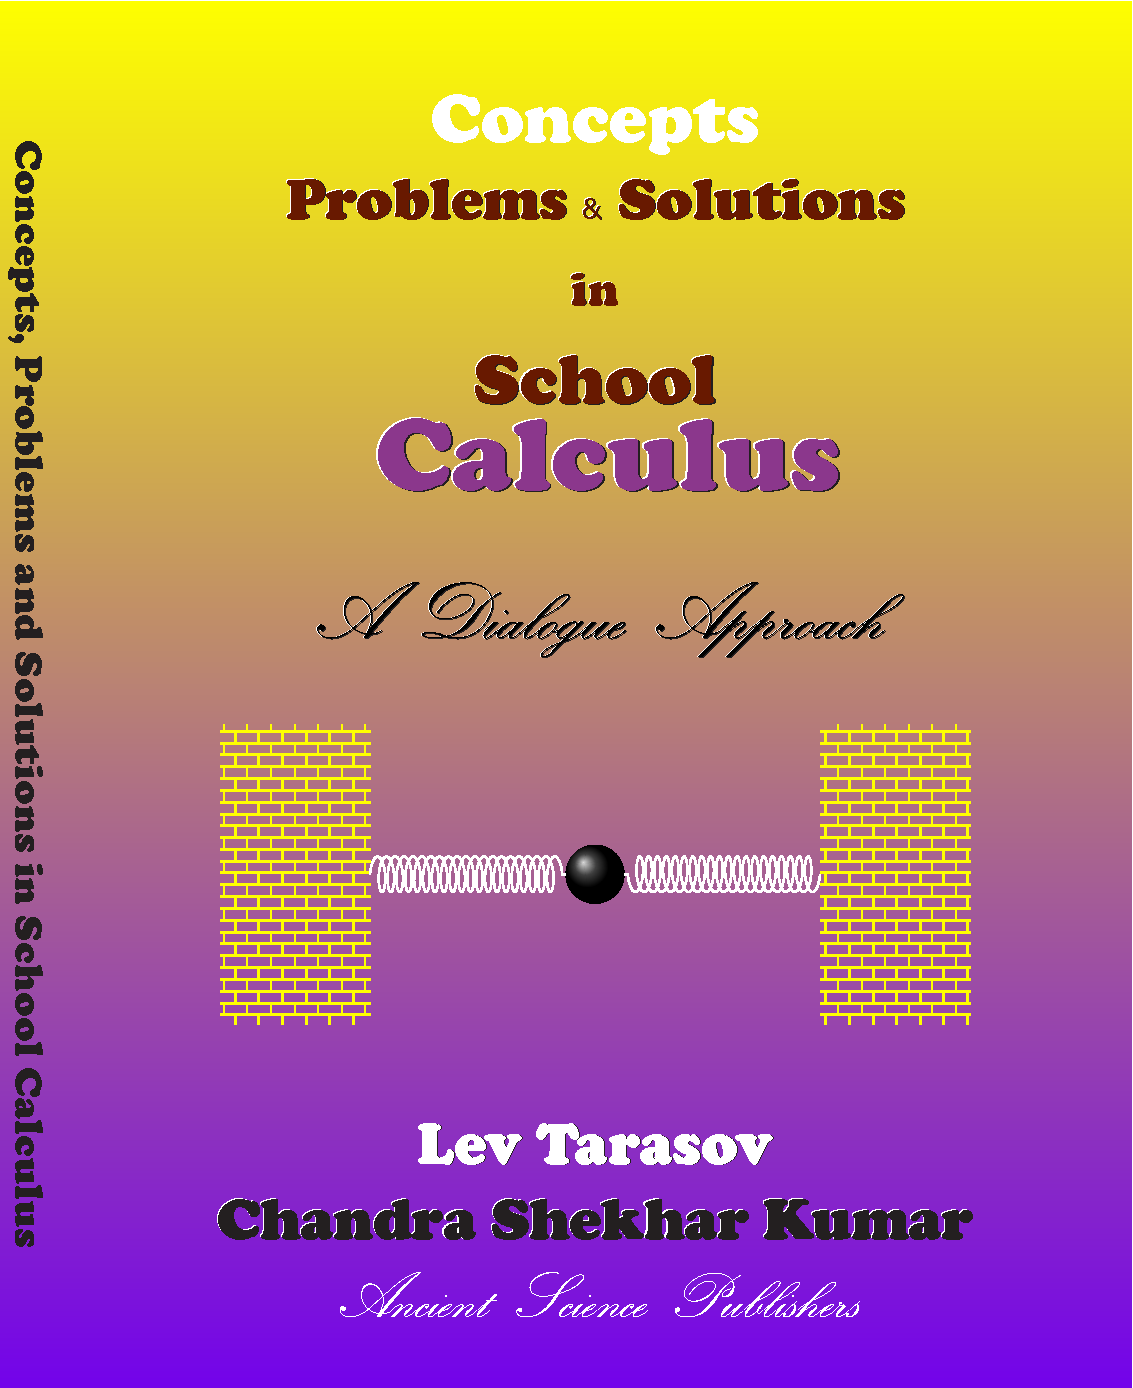
\includegraphics{solvingdpp//cover}

\chapter{Hacking TensorFlow Internals : An Insider’s Commentary on A Learning System}

\chapter{Advanced C++ FAQs Vol 1 \& 2}

\chapter{C++14 FAQs}

\begin{wrapfigure}{r}{0.5\textwidth}
  \begin{center}
    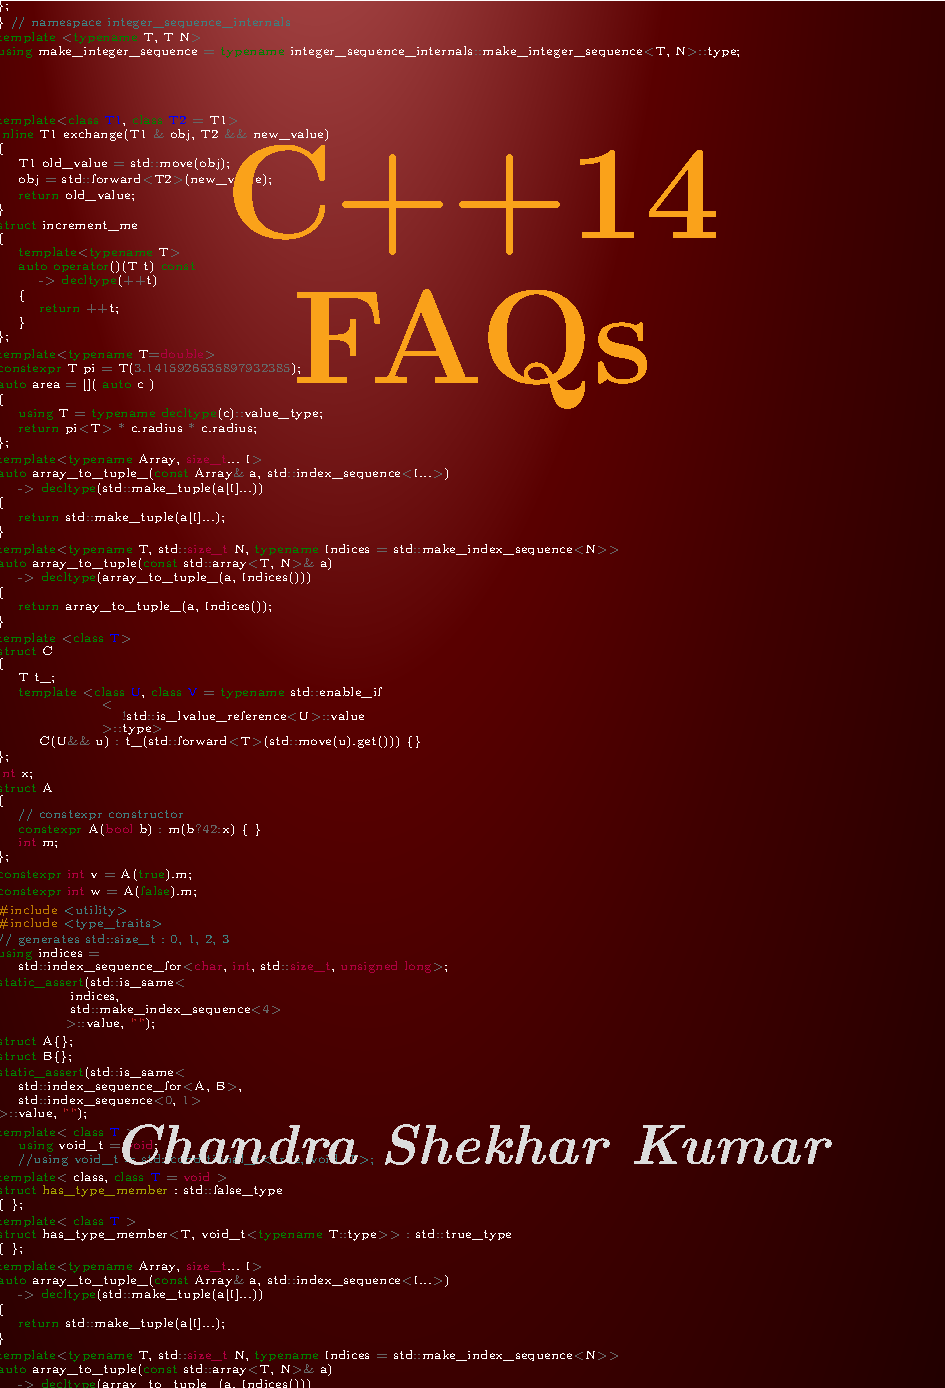
\includegraphics[width=0.5\textwidth]{cpp14faqs/cover}
  \end{center}
  %\caption{Front Cover}
\end{wrapfigure}

This book contains selected questions (84) related to C++14 with detailed solutions to all of these which will help the reader to hone her skills to solve a particular problem.

Primary source of this collection is \emph{Advanced C++ FAQs: Volumes 1 \& 2}.

This book is not an introduction to C++. It assumes that the reader is aware of the basics of C++98 and C++03 and wants to expand her horizon to latest and greatest in C++14(aka C++1y). The problems are marked on a scale of one(*)(simplest) to five stars(*****)(hardest).



\section{variable templates}


\begin{Exercise}[title={variable template}, difficulty=3, label=ex01]
\index{variable template}
What is a \emph{variable template} ?
\end{Exercise}



\begin{Answer}[ref=ex01]\index{variable template}
A \emph{variable template} is a declaration which is introduced by a template declaration of a variable. As we already know that a template declaration is also a definition if its declaration defines a function, a class, a variable, or a static data member.

A \emph{variable template} at class scope is a \emph{static data member template}.

Consider a simple template meta function, which uses variable template feature to store the boolean value of result of comparing two types:
\begin{lstlisting}
template <typename T, typename U>
constexpr bool is_same = std::is_same<T, U>::value;

bool t = is_same<int, int>; // true
bool f = is_same<int, float>; // false
\end{lstlisting}

The types of variable templates are not restricted to just built-in types; they can be user defined types.
\begin{lstlisting}
struct matrix_constants 
{
    template<typename T>
    using pauli = hermitian_matrix<T, 2>;
    
    template<typename T>
    constexpr pauli<T> sigma1 = { { 0, 1 }, { 1, 0 } };

    template<typename T>
    constexpr pauli<T> sigma2 = { { 0, -1i }, { 1i, 0 } };

    template<typename T>
    constexpr pauli<T> sigma3 = { { 1, 0 }, { -1, 0 } };
};
\end{lstlisting}

It makes definitions and uses of parameterized constants much simpler, leading to
simplified and more uniform programming rules to teach and to remember like:
\begin{lstlisting}
template<typename T>
struct lexical_cast_fn
{
    template<typename U>
    T operator()(U const &u) const
    {
        //...
    }
};

template<typename T>
constexpr lexical_cast_fn<T> lexical_cast{};

int main()
{
    lexical_cast<int>("42");
}
\end{lstlisting}

\end{Answer}



\section{Constexpr static data members of class templates}

\begin{Exercise}[title={\small Constexpr static data members of class templates}, difficulty=3, label=ex02]
\index{Constexpr static data members of class templates}
What is issue with constexpr static data members of class templates ?
\end{Exercise}


\begin{Answer}[ref=ex02]\index{Constexpr static data members of class templates}
Let us revisit how \emph{std::is\_same} is designed:

\begin{lstlisting}
template<typename T, T v>
struct integral_constant 
{
    static constexpr T value = v;
    typedef T value_type;
    ....
};

template<typename T, T v>
constexpr T integral_constant<T, v>::value;

typedef integral_constant<bool, true>  true_type;
typedef integral_constant<bool, false> false_type;

template<typename T, typename U>
struct is_same : false_type{};

template<typename T>
struct is_same<T, T> : true_type{};
\end{lstlisting}

The main problems with \emph{static data member} are:
\begin{itemize}
    \item they require \emph{duplicate} declarations: 
    \begin{enumerate}
        \item once inside the class template, 
        \item once outside the class template to provide the real definition in case the constants is odr(One Definition Rule) used.
    \end{enumerate}
    \item It creates confusion by the necessity of providing twice the same declaration, whereas ordinary constant declarations do not need duplicate declarations.
\end{itemize}

The standard class \emph{numeric\_limits} also suffers from the same problem as far as constexpr static data members are concerned.

\end{Answer}



\section{constexpr function templates}

\begin{Exercise}[title={constexpr function templates}, difficulty=3, label=ex03]
\index{constexpr function templates}
What is issue with constexpr function templates ?
\end{Exercise}


\begin{Answer}[ref=ex03]\index{constexpr function templates}
Constexpr functions templates provide functional abstraction.

A simple constexpr function template :
\begin{lstlisting}
template <typename T, typename U>
constexpr bool is_same()
{
    return std::is_same<T, U>::value;
}
\end{lstlisting}
Constexpr functions templates  do not have the duplicate declarations issue that static data members have.

However, they force us to chose in advance, at the definition site, how the constants are to be delivered: either by a const reference, or by plain non-reference type. 

If delivered by const reference then the constants must be systematically be allocated in static storage.

If by non-reference type, then the constants need copying. 

Copying isn't an issue for built-in types, but it is an issue for user-defined types with value semantics that aren't just wrappers around tiny built-in types

Whereas ordinary const(expr) variables do not suffer from this problem. A simple definition is provided, and the decision of whether the constants actually needs to be layout out in
storage only depends on the usage, not the definition.

Another examples are the static member functions of \emph{std::numeric\_limits} and functions like $boost::constants::pi<T>()$:
\begin{lstlisting}
#include <boost/math/constants/constants.hpp>

template <class Real>
Real area(Real r)
{
   using namespace boost::math::constants;
   return pi<Real>() * r * r;
}
\end{lstlisting}
The function template versions of the constants are simple inline functions that return a constant of the correct precision for the type used. In addition, these functions are declared constexpr for those compilers that support this, allowing the result to be used in constant expressions provided the template argument is a literal type. 

It looks like we are creating constexpr functions only to return a constant.

\end{Answer}




\section{variable templates in action}

\begin{Exercise}[title={variable templates in action}, difficulty=2, label=ex04]
\index{variable templates}
Illustrate how \emph{variable templates} can be used to compute the area of a circle for a given type with appropriate precision?
\end{Exercise}


\begin{Answer}[ref=ex04]\index{variable templates in action}
\emph{variable templates} address both of the issues illustrated before and no syntax modification was required to incorporate this feature in C++11 because current grammar allows any declaration to be parameterized. It was prohibited earlier via semantic constraints which is relaxed now on template declarations.

Let us first represent the mathematical constant $\pi$ with precision dictated by a floating point datatype:
\lstinputlisting[caption=$\pi$ and variable template]{cpp14faqs/code/c++14/variable_template.cpp}
With the following command:
\begin{verbatim}
clang++ -std=c++1y variable_template.cpp 
\end{verbatim}

we get the following output:
\begin{verbatim}
pi<int> : 3
pi<float> : 3.1415927410125732421875
pi<double> : 3.141592653589793115997963468544185161591
\end{verbatim}

This variable template can be used in a generic function to compute the area of a circle for a given radius:
\lstinputlisting{cpp14faqs/code/c++14/variable_template_area.cpp}

\end{Answer}




\section{static data member template}

\begin{Exercise}[title={static data member template}, difficulty=2, label=ex05]
\index{static data member template}
Provide a suitable definition of the static data member template \emph{min}:
\begin{lstlisting}
struct limits 
{
    template<typename T>
    static const T min; // declaration of min
};
\end{lstlisting}
\end{Exercise}


\begin{Answer}[ref=ex05]\index{static data member template}
As we already know that a variable template at class scope is a \emph{static data member template} and a definition for a static data member or static data member template may be provided in a namespace scope enclosing the definition of the static member's class template. 
\begin{lstlisting}
struct limits 
{
    template<typename T>
    static const T min; // declaration of min
};

template<typename T>
const T limits::min = { }; // definition of min
\end{lstlisting}
\end{Answer}



\section{specialization of variable template}

\begin{Exercise}[title={specialization of variable template}, difficulty=3, label=ex06]
\index{specialization of variable template}
Simplify the program below to do the needful:

\begin{lstlisting}
template <typename T, typename U>
constexpr bool is_same = std::is_same<T, U>::value;

bool t = is_same<int, int>; // true
bool f = is_same<int, float>; // false
\end{lstlisting}

\end{Exercise}


\begin{Answer}[ref=ex06]\index{specialization of variable template}
Variable templates are subject to template specialization like template functions, so we can simplify the code as follows:

\begin{lstlisting}
template<typename T, typename U>
constexpr bool is_same = false;

template<typename T>
constexpr bool is_same<T, T> = true;
\end{lstlisting}
\end{Answer}




\section{default argument and specialization of variable template}

\begin{Exercise}[title={\small default argument and specialization of variable template}, difficulty=3, label=ex07]
\index{default argument and specialization of variable template}
What is the output of the program ?
\lstinputlisting{cpp14faqs/code/c++14/specialize_variable_templates.cpp}

\end{Exercise}


\begin{Answer}[ref=ex07]\index{default argument and specialization of variable template}
\begin{verbatim}
pi<> : 3.14159265358979311599796346854
pi<int> : 3.1415927410125732421875
pi<float> : 3.1415927410125732421875
\end{verbatim}
\end{Answer}





\section{lambda and variable template}

\begin{Exercise}[title={\small lambda and variable template}, difficulty=3, label=ex08]
\index{lambda and variable template}

Simplify the program below.
\lstinputlisting{cpp14faqs/code/c++14/variable_template_area.cpp}

\end{Exercise}


\begin{Answer}[ref=ex08]\index{lambda and variable template}

\lstinputlisting{cpp14faqs/code/c++14/variable_template_simplify.cpp}

\end{Answer}





\section{variable templates variables vary}

\begin{Exercise}[title={variable templates variables vary}, difficulty=2, label=ex09]
\index{variable templates variables vary}

Is this a legal code ? 
\lstinputlisting{cpp14faqs/code/c++14/variable_template1.cpp}

If yes, what is the output ?

\end{Exercise}


\begin{Answer}[ref=ex09]\index{variable templates variables vary}

Yes, the code is correct because variable template instances are first-class objects.

Output is :
\begin{verbatim}
42
0
\end{verbatim}

\end{Answer}





\section{auto variable templates}

\begin{Exercise}[title={variable templates variables vary}, difficulty=2, label=ex010]
\index{auto variable templates}

Is this a legal code ? 
\lstinputlisting{cpp14faqs/code/c++14/auto_variable_templates.cpp}


\end{Exercise}


\begin{Answer}[ref=ex010]\index{auto variable templates}
Yes, a specialization of a variable template is a variable and as per the standard : \emph{No diagnostic shall be issued for a template for which a valid specialization can be generated}.

\end{Answer}





\section{valid specialization but error ?}

\begin{Exercise}[title={valid specialization but error}, difficulty=3, label=ex011]
\index{valid specialization but error}

Why this code doesn't compile ?
\lstinputlisting{cpp14faqs/code/c++14/specialize.cpp}


\end{Exercise}


\begin{Answer}[ref=ex011]\index{valid specialization but error}
Typical error is:
\begin{verbatim}
specialize.cpp:3:17: error: ‘typedef int Y::type’ is private
     typedef int type;
                 ^
specialize.cpp:6:13: error: within this context
 template<Y::type N>
             ^
\end{verbatim}
Because the template parameter declaration is ill-formed, it gets diagnosed immediately and does not form any larger structure. Hence there is no template to be specialized in the first place. There is no ``being ill-formed'', because ill-formedness implies the state of not being.

So, if the parameter is nonsensical, then we don't have a template declaration. And if the template declaration itself is nonsensical, we don't have a declaration to specialize, hencde the compiler error is issued.
\end{Answer}




\section{variable templates and lambda revisited}

\begin{Exercise}[title={variable templates and lambda revisited}, difficulty=3, label=ex012]
\index{variable templates and lambda revisited}

Exploit \emph{variable templates} and \emph{lambda} to compute the area of a circle class.

\end{Exercise}


\begin{Answer}[ref=ex012]\index{variable templates and lambda revisited}
\lstinputlisting{cpp14faqs/code/c++14/variable_template_lambda.cpp}

Alternatively:
\begin{lstlisting}
template<typename T>
using f_type = T(*)(Circle<T>);

template<typename T>
f_type<T> area = []( Circle<T> c ) 
{
    return pi<T> * c.radius * c.radius;
};
\end{lstlisting}

\end{Answer}



\section{Incremental improvement to integral\_constant}

\begin{Exercise}[title={\small Incremental improvement to integral\_constant}, difficulty=3, label=ex013]
\index{Incremental improvement to integral\_constant}
Revisit the class template \emph{is\_arithmetic}:
\begin{lstlisting}
template <class T> 
struct  is_arithmetic
    :  
    integral_constant<
    bool, 
    is_integral<T>::value ||
    is_floating_point<T>::value
 > {};
\end{lstlisting}

Before C++14, the typical usage of such a class template was:
\begin{lstlisting}
std::is_arithmetic<T>::value
\end{lstlisting}
or
\begin{lstlisting}
static_cast<bool>(std::is_arithmetic<T>{})
\end{lstlisting}

What was the increment improvement to the class \emph{integral\_constant} to enable simplified usage like
\begin{lstlisting}
std::is_arithmetic<T>{}()
\end{lstlisting}
\end{Exercise}


\begin{Answer}[ref=ex013]\index{Incremental improvement to integral\_constant}

The following addition was made in order to allow the template to serve as a source of compile-time function objects:
\begin{lstlisting}
constexpr value_type operator()() { return value; }
\end{lstlisting}
So the final class looked like:
\begin{lstlisting}
template <class T, T v>
struct integral_constant 
{
    static constexpr T value = v;
    using value_type = T;
    using type = integral_constant<T,v>;

    constexpr operator value_type() { return value; } 
    
    constexpr value_type operator()() { return value; } // C++14
};
\end{lstlisting}
\end{Answer}



\section{is\_same musings}

\begin{Exercise}[title={is\_same musing}, difficulty=2, label=ex014]
\index{is\_same musings}
Enumerate different ways to use $is\_same<T, U>$.
\end{Exercise}


\begin{Answer}[ref=ex014]\index{is\_same musing}

\begin{enumerate}
    \item As a function object:
    \begin{lstlisting}[numbers=none]
     std::is_same<T, U>()
    \end{lstlisting}
    \item As a compile time evaluation by invoking the nested \emph{value\_type}:
    \begin{lstlisting}[numbers=none]
    std::is_same<T, U>::value
    \end{lstlisting}
    \item By having a template alias as follows:
    \begin{lstlisting}[numbers=none]
    template<typename T, typename U>
    using is_same_v = typename std::is_same<T, U>::value;
    \end{lstlisting}
    Now we can use it like
     \begin{lstlisting}[numbers=none]
    is_same_v<T, U>()
    \end{lstlisting}
    \item In C++11:
    \begin{lstlisting}[numbers=none]
    static_cast<bool>(std::is_same<T, U>{})
    \end{lstlisting}
    \item Using variable template like:
    \begin{lstlisting}[numbers=none]
    template<typename T, typename U>
    constexpr bool is_same = false;

    template<typename T>
    constexpr bool is_same<T, T> = true;
    \end{lstlisting}
    It can be used like a variable:
     \begin{lstlisting}[numbers=none]
     is_same<T, U>
     \end{lstlisting}
\end{enumerate}

Note that in C++14, template aliases like the following are incorporated:
\begin{lstlisting}
template <class T, class U>
    using is_same_t = typename is_same<T, U>::type;
\end{lstlisting}
\end{Answer}






\section{auto variable template and generic lambda}

\begin{Exercise}[title={auto variable template and generic lambda}, difficulty=2, label=ex015]
\index{auto variable template and generic lambda}
Is this a valid code?
\lstinputlisting{cpp14faqs/code/c++14/generic_lambda3.cpp}
\end{Exercise}


\begin{Answer}[ref=ex015]\index{auto variable template and generic lambda}
Yes and it works as expected in C++14 and clang 3.5 trunk.
\end{Answer}







\section{constexpr member functions and implicit const}

\begin{Exercise}[title={constexpr member functions and implicit const}, difficulty=3, label=ex016]
\index{constexpr member functions and implicit const}
Review the program :
\lstinputlisting{cpp14faqs/code/c++14/constexpr_implicit_const.cpp}
\end{Exercise}


\begin{Answer}[ref=ex016]\index{constexpr member functions and implicit const}
Compiler error looks like:
\begin{verbatim}
constexpr_implicit_const.cpp: In function ‘int main()’:
constexpr_implicit_const.cpp:31:32: 
error: call to non-constexpr function ‘A& B::getA()’
     constexpr int n = B().getA().getN(); 
                                ^
\end{verbatim}

\emph{B().getA()} selects the non-constant overload version, leading to this error. 

After rendering the code as :
\lstinputlisting{cpp14faqs/code/c++14/constexpr_implicit_const1.cpp}

We get the following compiler error with C++11: clang++ -std=c++11
\begin{verbatim}
constexpr_implicit_const1.cpp:19:18: 
warning: 'constexpr' non-static member
      function will not be implicitly 'const' in C++1y; 
      add 'const' to avoid a
      change in behavior [-Wconstexpr-not-const]
    constexpr A &getA() 
                 ^
                        const
constexpr_implicit_const1.cpp:19:18: 
error: functions that differ only in their
      return type cannot be overloaded
constexpr_implicit_const1.cpp:15:24: 
note: previous declaration is here
    constexpr const A &getA() const
                       ^
constexpr_implicit_const1.cpp:21:16: 
error: binding of reference to type 'A' to
      a value of type 'const A' drops qualifiers
        return a; 
               ^
1 warning and 2 errors generated.
\end{verbatim}

It points to a couple of issues including the restriction that \emph{constexpr member functions are implicitly const in C++11} which creates problems for literal class types which desire to be usable both within constant expressions and outside them.

So in C++14, this rule is removed. So it works fine with C++14 compliant compiler like clang 3.5 trunk.

\end{Answer}






\section{constexpr constructor and initialization}

\begin{Exercise}[title={constexpr constructor and initialization}, difficulty=2, label=ex017]
\index{constexpr constructor and initialization}
Review the program :
\lstinputlisting{cpp14faqs/code/c++14/constexpr_constructor.cpp}
\end{Exercise}


\begin{Answer}[ref=ex017]\index{constexpr constructor and initialization}
Compiler error with gcc 4.9 trunk is:
\begin{verbatim}
constexpr_constructor.cpp:11:28:   
in constexpr expansion of ‘A(0)’
constexpr_constructor.cpp:11:28: 
error: the value of ‘x’ is not usable in a constant expression
 constexpr int w = A(false).m;       
                            ^
constexpr_constructor.cpp:1:5: note: ‘int x’ is not const
 int x;                              
     ^
\end{verbatim}
Compiler error with clang 3.5 trunk is:
\begin{verbatim}
constexpr_constructor.cpp:11:15: 
error: constexpr variable 'w' must be
      initialized by a constant expression
constexpr int w = A(false).m;       
              ^   ~~~~~~~~~~
constexpr_constructor.cpp:5:34: 
note: read of non-const variable 'x' is not
      allowed in a constant expression
    constexpr A(bool b) : m(b?42:x) { }
                                 ^
constexpr_constructor.cpp:11:19: note: in call to 'A(false)'
constexpr int w = A(false).m;       
                  ^
constexpr_constructor.cpp:1:5: note: declared here
int x;                              
    ^
1 error generated.
\end{verbatim}
The first call to constructor is ok it initializes m with the value $42$ whereas the second call is in error because initializer for $m$ is $x$, which is non-constant.
\end{Answer}



\section{constexpr and branching}

\begin{Exercise}[title={constexpr and branching}, difficulty=2, label=ex018]
\index{constexpr and branching}
Can we use if-then-else version of the following constexpr factorial program:
\begin{lstlisting}
constexpr unsigned long long fact( unsigned long long x ) 
{
    return x <= 1 ? 1ull : x * fact(x-1);
}
\end{lstlisting}
\end{Exercise}


\begin{Answer}[ref=ex018]\index{constexpr and branching}
C++14 allowed constexpr to include branching, so we can rewrite as follows:
\begin{lstlisting}
constexpr auto fact( unsigned long long x ) 
{
    if( x <= 1 )
        return 1ull;
    else
        return x * fact(x-1);
}
\end{lstlisting}
\end{Answer}



\section{constexpr and looping iteration}

\begin{Exercise}[title={constexpr and looping iteration}, difficulty=2, label=ex019]
\index{constexpr and looping iteration}
Can we use if-then-else version of the following constexpr factorial program:
\begin{lstlisting}
constexpr unsigned long long fact( unsigned long long x ) 
{
    return x <= 1 ? 1ull : x * fact(x-1);
}
\end{lstlisting}
\end{Exercise}


\begin{Answer}[ref=ex019]\index{constexpr and looping iteration}
C++14 allowed constexpr to support loop constructs, so we can rewrite the factorial program in its iterative version as follows:
\begin{lstlisting}
constexpr auto fact( unsigned long long x ) 
{
    auto product = x;
    
    while( --x )
        product *= x;
        
    return product;
}
\end{lstlisting}
C++11 requirement that constexprs be single return statements worked well enough, but simple functions that required more than one line could not be constexpr. It sometimes forced inefficient implementations in order to have at least some of its results generated at compile-time, but not always all. So this limitation was removed in C++14.

Note that this version may be more efficient, both at compile time and run time.
\end{Answer}



\section{constexpr and mutation}

\begin{Exercise}[title={constexpr and mutation}, difficulty=2, label=ex020]
\index{constexpr and initialization}
Review the program:
\lstinputlisting{cpp14faqs/code/c++14/constexpr_init.cpp}
\end{Exercise}


\begin{Answer}[ref=ex020]\index{constexpr and mutation}
It results into compiler error like:
\begin{verbatim}
constexpr_init.cpp:3:19: 
error: constexpr variable 'x' must be initialized by a
      constant expression
    constexpr int x = k;
                  ^   ~
constexpr_init.cpp:3:23: 
note: read of non-const variable 'k' is not allowed in
      a constant expression
    constexpr int x = k;
                      ^
constexpr_init.cpp:1:21: note: declared here
constexpr int f(int k) 
                    ^
1 error generated.

\end{verbatim}
The reason is : $x$ is not initialized by a constant expression because lifetime of $k$ began outside the initializer of $x$.

So the line 
\begin{lstlisting}[numbers=none]
constexpr int x = k;
\end{lstlisting}
should be replaced by:
\begin{lstlisting}[numbers=none]
int x = k;
\end{lstlisting}

To understand it better, let us review the following program:
\begin{lstlisting}
constexpr int incr(int &n) 
{
    return ++n;
}

constexpr int g(int k) 
{
    constexpr int x = incr(k);
    return x;
}
\end{lstlisting}
Here also, $incr(k)$ is not a core constant expression because lifetime of $k$ began outside the expression $incr(k)$, so the culprit line responsible for compiler error is:
\begin{lstlisting}
constexpr int x = incr(k);
\end{lstlisting}

Note that the following program is valid:
\begin{lstlisting}
constexpr int h(int k) 
{
    int x = incr(k);
    return x;
}
constexpr int y = h(1);
\end{lstlisting}
Because $h(1)$ is a core constant expression because the lifetime of $k$ begins inside $h(1)$. It initializes $y$ with the value $2$.

To summarize, C++14 allows \emph{mutation of objects whose lifetime began within the constant expression evaluation}.
\end{Answer}



\section{constexpr vs static vs uninitialized}

\begin{Exercise}[title={constexpr vs static vs uninitialized}, difficulty=2, label=ex021]
\index{constexpr vs static vs uninitialized}
Review the program:
\lstinputlisting{cpp14faqs/code/c++14/constexpr_static.cpp}
\end{Exercise}


\begin{Answer}[ref=ex021]\index{constexpr vs static vs uninitialized}
It does not compile. Typical error is, which is self-explanatory:
\begin{verbatim}
constexpr_static.cpp:3:16: 
error: static variable not permitted in a constexpr
      function
    static int value = n;         
               ^
constexpr_static.cpp:9:9: 
error: variables defined in a constexpr function must
      be initialized
    int a;                        
        ^
2 errors generated.
\end{verbatim}


\end{Answer}




\section{constexpr vs member function revisited}

\begin{Exercise}[title={constexpr vs member function revisited}, difficulty=2, label=ex022]
\index{constexpr vs member function revisited}
Is this code valid in C++14 ?
\lstinputlisting{cpp14faqs/code/c++14/constexpr_memfn.cpp}
\end{Exercise}


\begin{Answer}[ref=ex022]\index{constexpr vs member function revisited}
It was valid in C++11, but no more valid in C++14 because \emph{constexpr} non-static member functions are not implicitly const member functions anymore.

Rationale behind this change was \emph{to allow constexpr member functions to mutate the object}.

So the error is because it declares the same member function twice with different return types.

 Typical error is, which is self-explanatory:
\begin{verbatim}
constexpr_memfn.cpp:4:10: 
error: functions that differ only in their return type
      cannot be overloaded
    int &f();
         ^
constexpr_memfn.cpp:3:26: note: previous declaration is here
    constexpr const int &f();
                         ^
1 error generated.
\end{verbatim}


\end{Answer}




\section{deprecated attribute}

\begin{Exercise}[title={deprecated attribute}, difficulty=2, label=ex023]
\index{deprecated attribute}
Describe a mechanism to mark the usage of the class $A$ and the function $func1$ deprecated.
\begin{lstlisting}
class A1 {};

void func1() {}

int main()
{
    A1 a;
    func1();
}
\end{lstlisting}

\end{Exercise}


\begin{Answer}[ref=ex023]\index{deprecated attribute}
C++14 introduced an attribute \emph{[[deprecated]]} to do the needful. So we can rewrite the above code as:
\lstinputlisting{cpp14faqs/code/c++14/deprecated_attribute.cpp}

Compiler diagnostic messages with clang 3.5 trunk :
\begin{verbatim}
deprecated_attribute.cpp:8:5: warning: 'A1' is deprecated
      [-Wdeprecated-declarations]
    A1 a;
    ^
deprecated_attribute.cpp:1:22: 
note: 'A1' has been explicitly marked deprecated
      here
class [[deprecated]] A1 {};
                     ^
deprecated_attribute.cpp:9:5: warning: 'func1' is deprecated
      [-Wdeprecated-declarations]
    func1();
    ^
deprecated_attribute.cpp:4:6: 
note: 'func1' has been explicitly marked
      deprecated here
void func1() {}
     ^
2 warnings generated.
\end{verbatim}
With gcc 4.9 trunk:
\begin{verbatim}
deprecated_attribute.cpp: In function ‘int main()’:
deprecated_attribute.cpp:8:8: 
warning: ‘A1’ is deprecated 
(declared at deprecated_attribute.cpp:1) 
[-Wdeprecated-declarations]
     A1 a;
        ^
deprecated_attribute.cpp:9:5: 
warning: ‘void func1()’ is deprecated 
(declared at deprecated_attribute.cpp:4) 
[-Wdeprecated-declarations]
     func1();
     ^
deprecated_attribute.cpp:9:11: 
warning: ‘void func1()’ is deprecated 
(declared at deprecated_attribute.cpp:4)
 [-Wdeprecated-declarations]
     func1();
           ^
\end{verbatim}

The diagnostic message can be customized by passing a literal string as an argument to \emph{[[deprecated]]} like:
\lstinputlisting{cpp14faqs/code/c++14/deprecated_attribute_msg.cpp}
gcc 4.9 trunk yields now:
\begin{verbatim}
deprecated_attribute_msg.cpp: In function ‘int main()’:
deprecated_attribute_msg.cpp:8:8: 
warning: ‘A1’ is deprecated 
(declared at deprecated_attribute_msg.cpp:1): 
Usage of class A is deprecated. Please class X instead. 
[-Wdeprecated-declarations]
     A1 a;
        ^
deprecated_attribute_msg.cpp:9:5: 
warning: ‘void func1()’ is deprecated 
(declared at deprecated_attribute_msg.cpp:4): 
Usage of func1 is deprecated. Please use func2 instead. 
[-Wdeprecated-declarations]
     func1();
     ^
deprecated_attribute_msg.cpp:9:11: 
warning: ‘void func1()’ is deprecated 
(declared at deprecated_attribute_msg.cpp:4): 
Usage of func1 is deprecated. Please use func2 instead. 
[-Wdeprecated-declarations]
     func1();
           ^
\end{verbatim}
The attribute-token \emph{deprecated} can be used to mark names and entities whose use is still allowed, but is discouraged for some reason.

The attribute may be applied to the declaration of 
\begin{itemize}
\item a class, 
\item a typedef-name, 
\item a variable, 
\item a non-static data member, 
\item a function, 
\item an enumeration, or 
\item a template specialization.
\end{itemize}

A name or entity declared without the \emph{deprecated} attribute can later be redeclared with the attribute and vice-versa. 
\begin{lstlisting}
class A;
class [[deprecated]] A;

class A{};

int main()
{
    A a;
}
\end{lstlisting}

Compiler issues proper diagnostic.

Thus, an entity initially declared without the attribute can be marked as deprecated by
a subsequent redeclaration. 

However, after an entity is marked as deprecated, later redeclarations do not un-deprecate the entity.

So for the code below, compiler still issues the relevant diagnostics:
\begin{lstlisting}
class [[deprecated]] A;
class A;

class A{};

int main()
{
    A a;
}
\end{lstlisting}

Redeclarations using different forms of the attribute, with or without the attribute-argument-clause or with different attribute-argument-clauses) are allowed.
\lstinputlisting{cpp14faqs/code/c++14/deprecated_redeclare.cpp}
Compiler issues diagnostic message for the last one :
\begin{verbatim}
deprecated_redeclare.cpp:9:5: 
warning: 'A' is deprecated: A is dangerous.
      [-Wdeprecated-declarations]
    A a;
    ^
deprecated_redeclare.cpp:5:7: 
note: 'A' has been explicitly marked deprecated
      here
class A{};
      ^
1 warning generated.

\end{verbatim}
\end{Answer}



\chapter{The Boost C++ Libraries: Generic Programming}

\chapter{Generic Algorithms and Data Structures using C++11}

\chapter{C++11 Standard Library: Usage and Implementation}

\chapter{Foundation of Algorithms in C++11}

\chapter{C++11 Algorithms : Using and Extending C++11, Boost and Beyond}

\chapter{Cracking Programming Interviews : 500 Questions with Solutions}
\begin{wrapfigure}{r}{0.5\textwidth}
  \begin{center}
    
\includegraphics[width=0.5\textwidth]{cracking/cover}
  \end{center}
  %\caption{Front Cover}
\end{wrapfigure}

This book contains \textbf{500} programming questions most frequently asked in technical interviews in top technical companies including Facebook, Microsoft, Google, Apple, Yahoo and others. Detailed solutions are provided for all of these including tips and techniques for solving similar problems.


\section{Table of Contents}
\setlist{nosep}
\begin{enumerate}[label=\Roman*]
\item Algorithms and Data Structures
    \begin{enumerate}[label=\arabic*.]
      \item Fundamentals
          %\begin{enumerate}[label=\arabic{enumi}.\arabic*.]
          \begin{enumerate}[label*=\arabic*.]
              \item Approximating the square root of a number
              \item Generating Permutation Efficiently
              \item Unique 5-bit Sequences
              \item Select Kth Smallest Element
              \item The Non-Crooks Problem
              \item Is this (almost) sorted?
              \item Sorting an almost sorted list
              \item The Longest Upsequence Problem
              \item Fixed size generic array in C++
              \item Seating Problem
              \item Segment Problems
              \item Exponentiation
              \item Searching two-dimensional sorted array
              \item Initial bounded searcheable region
              \item Hamming Problem
              \item Constant Time Range Query
              \item Linear Time Sorting
              \item Writing a Value as the Sum of Squares
              \item The Celebrity Problem
              \item Transport Problem
              \item Find Length of the rope
              \item Switch Bulb Problem
              \item In, On or Out
              \item The problem of the balanced segments
              \item The problem of the most isolated villages
            \end{enumerate}  
      \item Arrays
          %\begin{enumerate}[label=\arabic{enumii}.\arabic*.]
          \begin{enumerate}[label*=\arabic*.]
              \item The Plateau Problem
              \item Searching in Two Dimensional Sequence
              \item The Welfare Crook Problem
              \item 2D Array Rotation
              \item A Queuing Problem in A Post Office
              \item Interpolation Search
              \item Robot Walk
              \item Linear Time Sorting
              \item Write as sum of consecutive positive numbers
              \item Print 2D Array in Spiral Order
              \item The Problem of the Circular Racecourse
              \item Sparse Array Trick
              \item Bulterman'{}s Reshuffling Problem
              \item Finding the majority
              \item Mode of a Multiset
              \item Circular Array
              \item Find Median of two sorted arrays
              \item Finding the missing integer
              \item Finding the missing number with sorted columns
              \item Re-arranging an array
              \item Switch and Bulb Problem
              \item Compute sum of sub-array
              \item Find a number not sum of subsets of array
              \item $K^{th}$ Smallest Element in Two Sorted Arrays
              \item Sort a sequence of sub-sequences
              \item Find missing integer
              \item Inplace Reversing
              \item Find the number not occurring twice in an array
            \end{enumerate}  
        \item Trees
          %\begin{enumerate}[label=\arabic{enumiii}.\arabic*.]
          \begin{enumerate}[label*=\arabic*.]
              \item Lowest Common Ancestor(LCA) Problem
              \item Path Number
              \item Spying Campaign
            \end{enumerate}  
        \item Dynamic Programming
          %\begin{enumerate}[label=\arabic{enumiv}.\arabic*.]
          \begin{enumerate}[label*=\arabic*.]
              \item Stage Coach Problem
              \item Matrix Multiplication
              \item TSP Problem
              \item A Simple Path Problem
              \item String Edit Distance
              \item Music recognition
              \item Max Sub-Array Problem
            \end{enumerate}  
        \item Graphs
          \begin{enumerate}[label*=\arabic*.]
              \item Reliable distribution
              \item Independent Set
              \item Party Problem
            \end{enumerate}    
        \item Miscellaneous
          \begin{enumerate}[label*=\arabic*.]
              \item Compute Next Higher Number
              \item Searching in Possibly Empty Two Dimensional Sequence
              \item Matching Nuts and Bolts Optimally
              \item Random-number generation
              \item Weighted Median
              \item Compute $a^{n}$
              \item Compute $a^{n}$ revisited
              \item Compute the product $a \times b$
              \item Compute the quotient and remainder
              \item Compute GCD
              \item Computed Constrained GCD
              \item Alternative Euclid'{} Algorithm
              \item Revisit Constrained GCD
              \item Compute Square using only addition and subtraction
              \item Factorization
              \item Factorization Revisited
              \item Decimal Representation
              \item Reverse Decimal Representation
              \item Solve Inequality
              \item Solve Inequality Revisited
              \item Print Decimal Representation
              \item Decimal Period Length
              \item Sequence Periodicity Problem
              \item Compute Function
              \item Emulate Division and Modulus Operations
              \item Sorting Array of Strings : Linear Time
              \item LRU data structure
              \item Exchange Prefix and Suffix
            \end{enumerate}    
        \item Parallel Algorithms
          \begin{enumerate}[label*=\arabic*.]
              \item Parallel Addition
              \item Find Maximum
              \item The Parallel Prefix Problem
              \item Finding Ranks in Linked Lists
              \item Finding the $k^{th}$ Smallest Element on a Tree
            \end{enumerate}    
        \item Low Level Algorithms
          \begin{enumerate}[label*=\arabic*.]
              \item Introduction
              \item Bit Counting Algorithms
              \item Rearranging Algorithms
              \item Computing Functions
              \item Miscellaneous
            \end{enumerate}    
        \end{enumerate}    
\item C++
    \begin{enumerate}[label=\arabic*]
      \item General
      \item Constant Expression
      \item Type Specifier
      \item Namespaces
      \item Misc
      \item Classes
      \item Templates
      \item Standard Library
    \end{enumerate}   
\end{enumerate} 

    

\hrulefill

\underline{\textbf{\textcolor{BurntOrange}{Excerpt from the Chapter} \textcolor{Sepia}{1:}}}

\section{Select Kth Smallest Element}\index{Select Kth Smallest Element}
\subsection*{Problem}
Design and implement an efficient algorithm to select the $K^{th}$ Smallest Element of an array.
\subsection*{Basic Analysis}
\subsubsection*{Simultaneous Min-Max Algorithm}
Before embarking on this selection problem, let us work out a general scheme of finding maximum and minimum of the input sequence. Min-max algorithms are ubiquitous in various applications specially geometric ones. In this section we will revisit several versions with primary focus being finding the most efficient one.

\vspace{1mm}

\emph{Design an efficient algorithm to find the minimum and maximum of an integer sequence simultaneously.}

\vspace{1mm}

Let us revisit a typical set-up for finding the maximum of an integer sequence where we end up examine each element of the sequence in turn along with keeping track of the largest element seen so far.

\begin{figure}[H]
\begin{center}
\fbox{\hlbt{Maximum of a sequence}}
\end{center}
\begin{algorithmic}[1]
\Function{maxval}{a, l, r}
    \State $0\le n$
    \State $a[k] \ge a[0..n - 1]$
    \State $i\gets 1$
    \State $k\gets 0$
 
    \While{$0\le n$}
        \If{$a[i] \le a[k]$}
            \State \emph{do nothing}
        \ElsIf{$a[i] \ge a[k]$}
            \State $k\gets i$
        \EndIf
        \State $i\gets i + 1$
    \EndWhile
    \State \textbf{return} $k$
\EndFunction
\end{algorithmic}
\end{figure}

\lstinputlisting[caption=Finding Maximum in an integer array]{cracking/minmax/maxvalarray.cpp}
As can be seen that this doesn\rq{}t address the scenario in presence of multiple occurrences. Let us put forth obvious solutions.
\lstinputlisting[caption=Finding First Maximum in an integer array]{cracking/minmax/firstmax.cpp}
\lstinputlisting[caption=Finding First Maximum Satisfying Predicate]{cracking/minmax/firstmax_if.cpp}
\lstinputlisting[caption=Finding First Minimum in an integer array]{cracking/minmax/firstmin.cpp}
Please note that :\\
\lstinputlisting[caption=Ordering Equivalence]{cracking/minmax/note1.hpp}
\lstinputlisting[caption=Finding Last Maximum in an integer array]{cracking/minmax/lastmax.cpp}
\lstinputlisting[caption=Finding Last Minimum in an integer array]{cracking/minmax/lastmin.cpp}
Please note that:\\
\lstinputlisting[caption=Another Ordering Equivalence]{cracking/minmax/note2.hpp}
\vspace{1mm}
All of these algorithms work in similar way requiring \emph{n - 1} comparisons in worst case.

\vspace{1mm}

How about simultaneously finding maximum and minimum of the sequence? 

Naively, we can get this done in two passes : once for finding maximum and another for finding minimum : total of \emph{2n - 2} comparisons. But we can definitely do better if we confine ourselves to a single pass and reply on maintaining maximum and minimum elements seen so far. Instead of picking one element and probing it against the current maximum or minimum, we can rather examine two elements at a time treating them as pairs. The process goes like this:
\begin{enumerate}
    \item Maintain the minimum and maximum of elements seen so far.
    \item Don\rq{}t compare each element to the minimum and maximum separately, which requires two comparisons per element.
    \item Pick up the elements in pairs.
    \item Compare the elements of a pair to each other.
    \item Then compare the larger element to the maximum so far, and compare the
smaller element to the minimum so far. 
\end{enumerate}
The above requires only three comparisons per two elements. Setting up the initial values for the min and max depends on whether n is odd or even.
\begin{itemize}
    \item If n is even, compare the first two elements and assign the larger to max and the smaller to min. \vspace{1mm}\\This needs one initial comparison and then $\frac{3(n - 2)}{2}$ more comparisons. Thus total number of comparisons = \vspace{1mm}\\ 1 + $\frac{3(n - 2)}{2}$\\ = 1 + $\frac{3n - 6}{2}$\\ = 1 + $\frac{3n}{2}$ - 3\\ =  $\frac{3n}{2}$ - 2. \vspace{1mm}\\Then process the rest of the elements in pairs. 
    \item If n is odd, set both min and max to the first element. Then process the rest of the elements in pairs. This needs a total of $\frac{3(n - 1)}{2}$ comparisons.
\end{itemize}

\lstinputlisting[caption=C++ Implementation of first min and first max]{cracking/minmax/firstmin_firstmax.cpp}
Please note that only one comparison is required for first two elements(aka first pair). The above requires at most three comparisons per pair.

\vspace{1mm}

In similar spirit, there are multiple combinations possible like:
\begin{itemize}
    \item first\_min\_first\_max\_element
    \item first\_min\_last\_max\_element
    \item last\_min\_first\_max\_element
    \item last\_min\_last\_max\_element
\end{itemize}
Let us look at the implementation of \\first\_min\_last\_max\_element as inspiration.
\lstinputlisting[caption=first\_min\_last\_max\_element]{cracking/minmax/firstmin_lastmax.cpp}

\subsubsection*{Generic Select}
Selection can be reduced to sorting by sorting the sequence and then extracting the sought after element. This method is more efficient when many selections need to be made from a sequence, in which case only one initial, so-called expensive sort is needed, followed by many relatively less expensive extraction operations, usually in amortized constant time. In general, this method requires $O(n \log n)$ time, where \emph{n} is the length of the sequence.

\vspace{1mm}

Let us try using similar ideas as in finding minimum and maximum of a given sequence for finding the $k^{th}$ smallest or $k^{th}$ largest element in a sequence.

\begin{figure}[H]
\begin{center}
\fbox{\hlbt{Generic Kth Select Minimum}}
\end{center}
\begin{algorithmic}[1]
\Function{generic-kth-min-select}{a, l, r, k}
    \State $numElements \gets r - l + 1$
    \For{$i \gets 1$, $k$}
        \State $minIndex \gets i$
        \State $minVal \gets a[i]$
        \For{$j \gets i + 1, numElements$}
            \If{$a[j] < minVal$}
                \State $minIndex \gets j$
                \State $minVal \gets a[j]$
            \EndIf
        \EndFor
            \State $swap(a[i], a[minIndex])$
        \EndFor
    \State \textbf{return} $a[k]$
\EndFunction
\end{algorithmic}
\end{figure}

\lstinputlisting[caption=Generic Kth Select Minimum]{cracking/select/generic_minselect.cpp}
As can be seen  that time complexity of this inefficient selection algorithm is $O(kn)$, where n is the length of the sequence, which is acceptable when \emph{k} is small enough. It works by simply finding the most minimum element and moving it to the beginning until we reach our desired index, i.e., \emph{k}. It resembles a \emph{partial selection sort}.

\subsection*{Randomized Quick Select Algorithm}\index{randomized quick select}
Let us recall \emph{\textsc{randomized-partition}} and \emph{\textsc{randomized-quicksort}} algorithms to help us build an efficient selection algorithm. 
\begin{figure}[H]
\begin{center}
\fbox{\hlbt{Partitioning a sequence}}
\end{center}
\begin{algorithmic}[1]
\Function{partition}{a, l, r}
    \State $p\gets a[r]$
    \State $i \gets l - 1$
    \For{$j \gets l$, $r - 1$}
        \If{$a[j] \le p$}
            \State $i \gets i + 1$
            \State $swap(a[i], a[j])$
        \EndIf
    \EndFor
    \State \textbf{return} $i + 1$
\EndFunction
\end{algorithmic}
\end{figure}

\begin{figure}[H]
\begin{center}
\fbox{\hlbt{Randomized Partition Algorithm}}
\end{center}
\begin{algorithmic}[1]
\Function{randomized-partition}{a, l, r}
    \State $i \gets random(l, r)$
    \State $swap(a[r], a[i])$  
  \State \textbf{return} \textsc{partition}$(a, l, r)$
\EndFunction
\end{algorithmic}
\end{figure}

\begin{figure}[H]
\begin{center}
\fbox{\hlbt{Randomized Quicksort Algorithm}}
\end{center}
\begin{algorithmic}[1]
\Function{randomized-quicksort}{a, l, r}
    \State $p \gets$ \textsc{randomized-partition}$(a, l, r)$
    \State \textsc{randomized-quicksort}$(a, l, p - 1)$
    \State \textsc{randomized-quicksort}$(a, p + 1, r)$  
\EndFunction
\end{algorithmic}
\end{figure}

Let us model the algorithm \emph{randomized-select} based on \emph{randomized-quicksort}, but unlike quicksort, which involves partitioning the input array followed by processing both sides of the partition recursively, \emph{randomized-select} works on only one side of the partition, thus throwing away the other partition.

\subsection*{Algorithm}

\begin{figure}[H]
\begin{center}
\fbox{\hlbt{Randomized Kth Min Select Algorithm}}
\end{center}
\begin{algorithmic}[1]
\Function{randomized-kth-min-select}{a, l, r, k}
    \State $p \gets$ \textsc{randomized-partition}$(a, l, r)$
    \State $pdist \gets p - l + 1$
    \If{k == mid}
        \State \textbf{return} $a[p]$
    \ElsIf{k < pdist}
        \State \textbf{return} \textsc{randomized-kth-min-select}$(a, l, p - 1, k)$
    \ElsIf{k > pdist}
        \State \textbf{return} \textsc{randomized-kth-min-select}$(a, p + 1, r, k - pdist)$  
    \EndIf
\EndFunction
\end{algorithmic}
\end{figure}

And it is not that difficult to see that average case time complexity of the algorithm \emph{\textsc{randomized-kth-min-select}} is $\Theta(n)$ and worst case time complexity is $\Theta(n^{2})$, assuming that the elements are distinct.

\subsection*{C++11 Implementation}
\lstinputlisting[caption=Randomized version of Kth Select Minimum]{cracking/select/randomized_select.cpp}

\emph{\textsc{randomized-kth-min-select}} differs from\\ \emph{\textsc{randomized-quicksort}} because it recurses on one side of the partition only. After the call to \emph{\textsc{randomized-partition}}, the sequence $a[l..r]$ is partitioned into two sub-sequences $a[l..p - 1]$ and $a[p + 1..r]$, along with a pivot element $a[p]$.
\begin{itemize}
    \item The elements of sub-sequence $a[l..p - 1]$ are all $ \le a[p]$.
    \item The elements of sub-sequence $a[p + 1.. r]$ are all $ > a[p]$.
    \item The pivot element is the $pdist^{th}$ element of the sub-sequence $a[l..r]$, where $pdist = p − l + 1$.
    \item If the pivot element is the $k^{th}$ smallest element (i.e., k = pdist), return A[p].
    \item Otherwise, recurse on the sub-sequence containing the $k^{th}$ smallest element.
    \begin{itemize}
        \item If $k < pdist$, this sub-sequence is $a[l..p - 1]$ and we want the  $k^{th}$ smallest element.
        \item If $k > pdist$, this sub-sequence is $a[p + 1.. r]$ and, since there are \emph{pdist} elements in $a[l..r]$ that precede $a[p + 1.. r]$, we want the $(k - pdist)^{th}$ smallest element of this sub-sequence.
    \end{itemize}
\end{itemize}
It resembles a \emph{partial quicksort}\index{partial quicksort}, generating and partitioning only $O(\log n)$ of its $O(n)$ partitions. This simple algorithm has expected linear performance, and, like quicksort, has quite good performance in practice. It is also an \emph{in-place} algorithm, requiring only constant memory overhead, since the tail recursion can be eliminated with an equivalent iterative version as shown in the next section. In a \emph{tail recursion}, the call is always the last action in an algorithm. A tail-recursive algorithm can always be transformed into an equivalent iterative algorithm with a \emph{while} loop as shown ahead.

\subsection*{Iterative Version of Quick Select Algorithm}\index{quick select iterative}
\begin{figure}[H]
\begin{center}
\fbox{\hlbt{Iterative Version of Quick Select Algorithm}}
\end{center}
\begin{algorithmic}[1]
\Function{randomized-kth-min-select}{a, l, r, k}
    \While{l < r}
        \State $p \gets$ \textsc{randomized-partition}$(a, l, r)$
        \State $pdist \gets p - l + 1$
        \If{k == mid}
            \State \textbf{return} $a[p]$
        \ElsIf{k < pdist}
            \State $r \gets p - 1$
        \ElsIf{k > pdist}
            \State $l \gets p + 1$
            \State $k \gets k - pdist$  
        \EndIf
    \EndWhile
\EndFunction 
\end{algorithmic}
\end{figure}






\chapter{Top 20 Coding Interview Problems Asked in Google with Solutions}
\begin{wrapfigure}{r}{0.5\textwidth}
  \begin{center}
    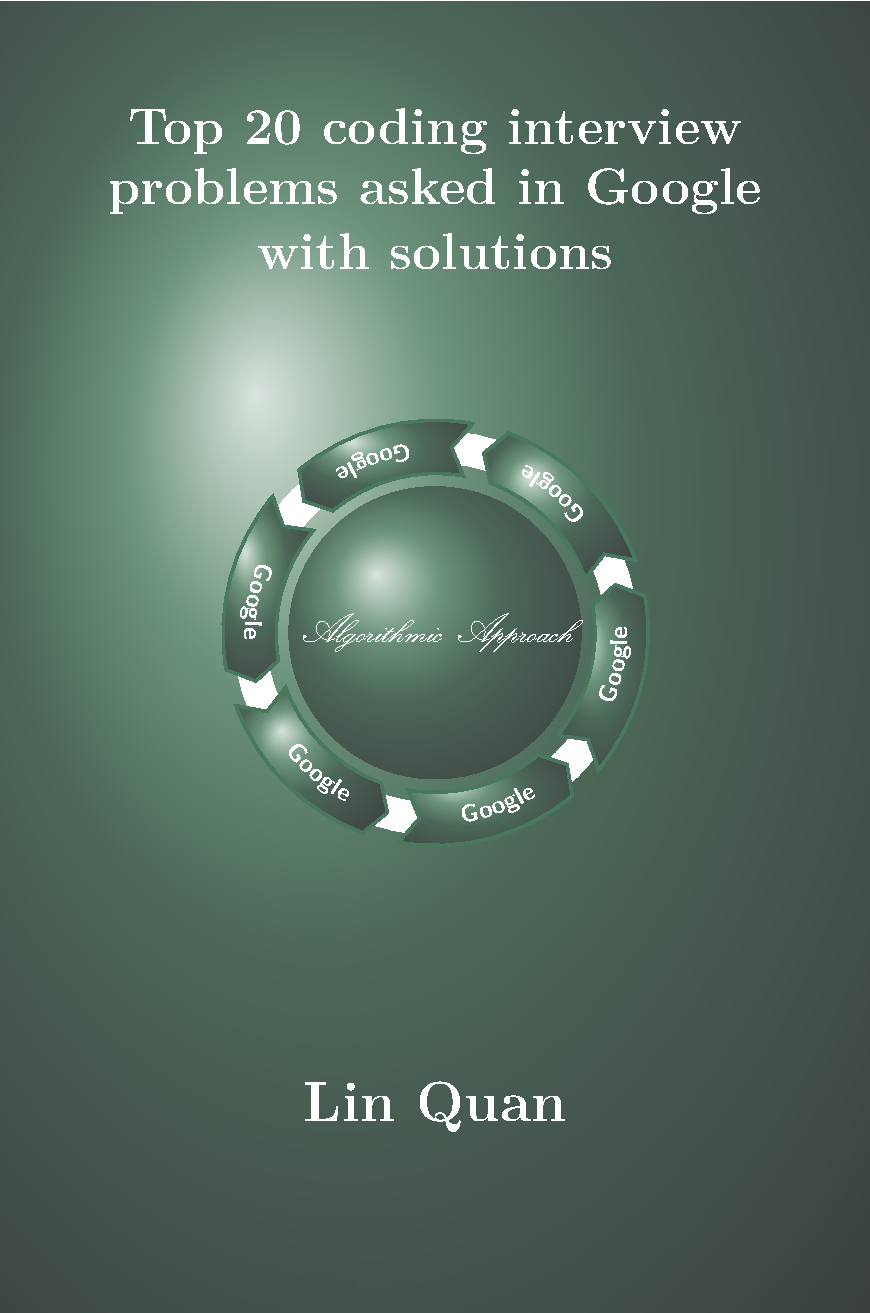
\includegraphics[width=0.5\textwidth]{top20/cover}
  \end{center}
  %\caption{Front Cover}
\end{wrapfigure}

This book is written for helping people prepare for Google Coding Interview. It contains top 20 programming problems frequently asked @Google with detailed worked-out solutions both in pseudo-code and C++ (and C++11).

It came out as a result of numerous requests received from coders across the Globe, primarily from Google aspirants. Author has a vast collection of algorithmic problems since 20 years including experience in preparing computer science students for participation in programming contests like TopCoder, ACM ICPC and others.



\begin{center}
\textbf{Must Have for Google Aspirants !!!}
\end{center}

\colorlet{BgTextColor}{Sepia} 

%\begin{comment}
\begin{enumerate}[nosep]
\itemcolor{BgTextColor}
\item \emph{\textcolor{BgTextColor}{Matching Nuts and Bolts Optimally}}
\item \emph{\textcolor{BgTextColor}{Searching two-dimensional sorted array}}
\item \emph{\textcolor{BgTextColor}{Lowest Common Ancestor(LCA) Problem}}
\item \emph{\textcolor{BgTextColor}{Max Sub-Array Problem}}
\item \emph{\textcolor{BgTextColor}{Compute Next Higher Number}}
\item \emph{\textcolor{BgTextColor}{2D Binary Search}}
\item \emph{\textcolor{BgTextColor}{String Edit Distance}}
\item \emph{\textcolor{BgTextColor}{Searching in Two Dimensional Sequence}}
\item \emph{\textcolor{BgTextColor}{Select Kth Smallest Element}}
\item \emph{\textcolor{BgTextColor}{Searching in Possibly Empty Two Dimensional Sequence}}
\item \emph{\textcolor{BgTextColor}{The Celebrity Problem}}
\item \emph{\textcolor{BgTextColor}{Switch and Bulb Problem}}
\item \emph{\textcolor{BgTextColor}{Interpolation Search}}
\item \emph{\textcolor{BgTextColor}{The Majority Problem}}
\item \emph{\textcolor{BgTextColor}{The Plateau Problem}}
\item \emph{\textcolor{BgTextColor}{Segment Problems}}
\item \emph{\textcolor{BgTextColor}{Efficient Permutation}}
\item \emph{\textcolor{BgTextColor}{The Non-Crooks Problem}}
\item \emph{\textcolor{BgTextColor}{Median Search Problem}}
\item \emph{\textcolor{BgTextColor}{Missing Integer Problem}}
\end{enumerate}
%\end{comment}

%\newcommand\problem[1]{{#1}}

%\newcommand\solution[1]{{#1}}

%\renewcommand{\ExerciseName}{Problem}
%\renewcommand{\AnswerName}{Solution}
%\renewcommand{\AnswerHeader}{\centerline{\textbf{\Large \solution{\AnswerName}}}}

%\renewcommand{\ExerciseHeader}{\problem{\centerline{\textbf{\Large  \ExerciseName\hspace{1mm}\ExerciseHeaderNB\ExerciseHeaderTitle \small \ExerciseHeaderOrigin\medskip}}}}


\underline{\textbf{\textcolor{BurntOrange}{Excerpt from the Chapter} \textcolor{Sepia}{2:}}}

\section{Searching two-dimensional sorted array}

%\begin{Exercise}[difficulty=2, origin=David Gries, label=twod]
\begin{center}
\hlbt{**\textsc{Problem} 2 (\small David Gries)}
\end{center}
\hlt{Design and implement an efficient algorithm to search for a given integer x in a 2-dimensional \textbf{sorted} array a[0..m][0..n]. Please note that it is sorted row-wise and column-wise in ascending order.}
%\end{Exercise}

\begin{center}
\hlbt{\textsc{Solution}}
\end{center}

%\begin{Answer}[ref=twod]

\subsection{Basic Analysis}

\noindent \qquad Let us start analyzing the problem by looking at implied properties related to search space. This array has the following properties:
\begin{enumerate}
    \item no of rows $m \geq 1$
    \item no of columns  $n \geq 1$
    \item Entries in each row are ordered by $\leq$, i.e., for $0 \leq i < m$ \&\& $0 \leq j < n$ 
    \vspace{1mm}\\
    \fbox{$\mathbf{a[i][j] \leq a[i][j+1]}$}
    \begin{itemize}
        \item $a_{11} \leq a_{12} \leq \ldots \leq a_{1n}$
        \item $a_{21} \leq a_{22} \leq \ldots \leq a_{2n}$
        \vspace{1mm}\\\vdots
        \item $a_{m1} \leq a_{m2} \leq \ldots \leq a_{mn}$
    \end{itemize}
    \item Entries in each column are ordered by $\leq$, i.e., for $0 \leq i < m$ \&\& for $0 \leq j < n$\vspace{1mm}\\
    \fbox{$\mathbf{a[i][j] \leq a[i+1][j]}$}
        \begin{itemize}
        \item $a_{11} \leq a_{21} \leq \ldots \leq a_{m1}$
        \item $a_{12} \leq a_{22} \leq \ldots \leq a_{m2}$
        \vspace{1mm}\\\vdots
        \item $a_{1n} \leq a_{2n} \leq \ldots \leq a_{mn}$
    \end{itemize}
\end{enumerate}


Pictorial representation of two-dimensional sorted array is as follows:
\begin{center}
\begin{tikzpicture}
%\tikzstyle{ball} = [circle, shading=ball, ball color=black!80!white, minimum size=1cm, text=white]
\tikzstyle{ball} = [circle, fill=black!80!white, minimum size=1cm, text=white]

\matrix [matrix of math nodes, nodes=ball]
{
a_{11} & a_{12} & \ldots & a_{1n} \\
a_{21} & a_{22} &  \ldots & a_{2n}\\
\vdots & \vdots & \ddots & \vdots\\
a_{m1} & a_{m2} & \ldots & a_{mn} \\
};
\end{tikzpicture}
\end{center}

With the properties above, we have to develop an efficient algorithm to find the position of a given integer x in the array a, i.e., the algorithm should find i and j such that  \fbox{$\mathbf{x = a[i, j]}$}. By efficient we mean to minimize the number of comparisons as much as possible.
\vspace{3mm}\\
Let us treat the input array as some kind of a rectangular region. 
\vspace{3mm}\\
The problem demands that the integer $x$ does exist somewhere in this region. Let us label this condition as \emph{Input Assertion} or \emph{Precondition}.\index{precondition}

\subsection{Precondition (aka \textit{Input Assertion})}

\fbox{$\mathbf{x \in a[0..m-1, 0..n-1]}$} \vspace{1mm}\\
i.e., x is present somewhere in this rectangular region $a$.

\begin{center}
\begin{tikzpicture}

\node at (0,0) (a1) {};
\node at (3,2) (a2) {};
\node[draw=black,inner sep=2mm,thick,rectangle,fit=(a1) (a2)] (a) {$x$};
\node[above] at (a.north west) {$0$};
\node[below] at (a.south west) {$m-1$};
\node[above] at (a.north east) {$n-1$};

\end{tikzpicture}
\end{center}

After the program terminates successfully, $x$ has to be found in a rectangular region of $a$ where the rectangular region consists of just one row and column. Let us label this condition as \emph{Output Assertion} or \emph{Result Assertion} or \emph{Postcondition}.\index{postcondition}

\subsection{Postcondition (aka \textit{Result Assertion)}}

\fbox{$\mathbf{0 \leq i \leq m-1}$} \&\& \fbox{$\mathbf{0 \leq j \leq n-1}$} \&\& \fbox{ $\mathbf{x = a[i, j]}$} \vspace{1mm}\vspace{1mm}\\
i.e., x is in a rectangular region of $a$ where the rectangular region consists of just one row and column, i.e., $x$ is present at $i^{th}$ row and $j^{th}$ column of $a$.
 
\begin{center}
\begin{tikzpicture}

\node at (0,0) (a1) {};
\node at (3,2) (a2) {};
\node[draw=black,inner sep=2mm,thick,rectangle,fit=(a1) (a2)] (a) {$x$};
\node[above] at (a.north west) {$0$};
\node[left] at (a.west) {$i$};
\node[below] at (a.south west) {$m-1$};
\node[above] at (a.north) {$j$};
\node[above] at (a.north east) {$n-1$};

\end{tikzpicture}
\end{center}

\subsection{Invariant} \index{variant}
Looking at the precondition and postcondition, it is not that difficult to figure out that during the execution of our algorithm, x is guaranteed to be confined within some rectangular region of $a$, i.e., 
\vspace{1mm} \\
\fbox{$\mathbf{0 \leq i \leq p \leq m-1}$} \&\& \\\fbox{$\mathbf{0 \leq q \leq j \leq n-1}$} \&\& \\\fbox{$\mathbf{x \in a[i..p, q..j]}$}.
\vspace{1mm}\\
In simple words, the invariant implies that 
\begin{itemize}
    \item We have exhausted the rows a[0..p-1] and x is not present in these already searched rows.
    \item We have exhausted the columns a[0..q-1] and x is not present in these already searched columns.
\end{itemize}

\begin{center}
\begin{tikzpicture}

\node at (0,0) (a1) {};
\node at (3,2) (a2) {};
\node[draw=black,inner sep=2mm,thick,rectangle,fit=(a1) (a2)] (a) {};
\node[above] at (a.north west) {$0$};

\node[shift=(a.160), left] at (a.west) {$i$};

\node[left] (p) at (a.west) {$p$};

\draw[densely dashdotdotted] (a.west) -- (a.mid);

\node[below] at (a.south west) {$m-1$};
\node[shift=(a.70), above] at (a.north) {$j$};

\node[above] at (a.north) {$q$};

\draw[densely dashdotdotted] (a.north) -- (a.mid);

\node[below] at (18pt, 55pt) {x not found};

\node[above] at (a.north east) {$n-1$};

\end{tikzpicture}
\end{center}


\subsection{Contract the rectangular region}
We have to choose a rectangular region $a[i..p, q..j]$ that contains x followed by making this region smaller till x is found. 
\paragraph{Initial bounded searcheable region} is represented by : \\
$i = 0$\hspace{1.2mm} $p = m - 1$\hspace{1.2mm} $q = 0$\hspace{1.2mm} 
$j=n - 1$\vspace{2mm}\\
Looking at bounds of the rectangle, there are 4 ways to march towards contracting it:


\begin{itemize}
    \item if $a[i, j] < x$ then since the row is ordered $\implies$ $i \leftarrow i + 1$, because if $a[i, j] > x$, then all the entries of that row is also greater than x. Please note that its execution will maintain the stated invariant if $x$ is not found in a[i, 0..n-1], i.e., in $i^{th}$ row.
    \item if $a[p, q] > x$ $\implies$ $p \leftarrow p - 1$
    \item if $a[p, q] < x$ $\implies$ $q \leftarrow q + 1$
    \item if $a[i, j] > x$ $\implies$ $j \leftarrow j - 1$
\end{itemize}

These conditions are also known as \textit{guards}\cite{gries}.



\subsection{Saddleback Search Algorithm}\index{saddleback search}
Let us put together the complete solution as shown below:

\begin{figure}[H]
\begin{center}
\fbox{\hlbt{Saddleback Search Algorithm}}
\end{center}
\begin{algorithmic}[1]
\State \textbf{PreCondition}{ : $x \in a[0..m-1, 0..n-1]$}
\State \textbf{PostCondition}{ : $0 \leq i \leq m-1$ \&\& $0 \leq j \leq n-1$ \&\& $x = a[i, j]$}
\Function{Saddleback-search}{a[0..m-1, 0..n-1], x}
    \State $i \gets 0$
    \State $p \gets m - 1$
    \State $q \gets 0$
    \State $j \gets n - 1$
  \State \textbf{Invariant}{ : $0 \leq i \leq p \leq m-1$ \&\& $0 \leq q \leq j \leq n-1$ \&\& $x \in a[i..p, q..j]$}\vspace{1mm}     
  \While{$x \neq a[i, j]$}
    \If{a[i, j] < x}
        \State  $i \longleftarrow i + 1$
    \EndIf
    \If{a[p, q] > x}
        \State  $p \longleftarrow p - 1$
    \EndIf
    \If{a[p, q] < x}
        \State  $q \longleftarrow q + 1$
    \EndIf
    \If{a[i, j] > x}
        \State  $j \longleftarrow j - 1$
    \EndIf
   \EndWhile
\EndFunction
\end{algorithmic}
\end{figure}


This layout was simple enough to embark on the journey of solving problems using formal programming methodology in somewhat pragmatic manner. 
\vspace{1mm}\\
With the above setting in place, now it is time to think towards proving correctness of the result upon termination. As an astute reader, it is not that difficult to surmise that intermediate conditions in form of the points p,q of search space are not really needed to test veracity of the result upon termination. Only the first and last conditions are necessary and sufficient enough to prove it. So let us drop the middle (two) conditions to complete the working program in practice as following:

\begin{figure}[H]
\begin{center}
\fbox{\hlbt{Saddleback Search Algorithm in practice}}
\end{center}
\begin{algorithmic}[1]
\State \textbf{PreCondition}{ : $x \in a[0..m-1, 0..n-1]$}
\State \textbf{PostCondition}{ : $0 \leq i \leq m-1$ \&\& $0 \leq j \leq n-1$ \&\& $x = a[i, j]$}
\State \textbf{Invariant}{ : x is in a[i..m-1, 0..j]}
\Function{Saddleback-search}{a[0..m-1, 0..n-1], x}
        \While{$x \neq a[i, j]$}
            \If{a[i, j] < x}
                \State $i \gets i + 1$
                \Else $j \gets j - 1$
            \EndIf
        \EndWhile
\EndFunction
\end{algorithmic}
\end{figure}

Still, we need to address that why we chose to start from top rightmost corner. We can of course start from bottom leftmost corner as well. We leave this an exercise to the reader to work out and think about the pros n cons of choosing the starting point.

\subsubsection{C++11 Implementation}

Let us try programming this algorithm in a real language, say C++11 to bring ourselves at workplace-setting environment:

\lstinputlisting[caption=Saddleback search in C++11]{top20/saddle/saddleback_search.hpp}

\lstinputlisting[caption=Using Saddleback Search]{top20/saddle/saddleback_search_test1.cpp}
Output of the program is:
\begin{boxedverbatim}
6 is found at : a[1][3]
\end{boxedverbatim}
\subsubsection{Time Complexity} 
As could be seen that the number of comparisons required in Saddleback search algorithm is at most $n + m$. Hence time complexity is $O(n + m)$. 
\vspace{1mm}\\
How to improve it further, is it possible? 
\vspace{1mm}\\
Let us take a simple case as a tryst to understand it better. Let us assume that the array is a square one with n x n dimension, i.e., m = n. Please note that the elements lying off-diagonal in the rectangular region form an unordered sequence of integers, i.e., a[0, n-1], a[1, n-2], a[2, n-3], $\ldots$, a[n-2, 1] and a[n-1, 0] form an unordered list because this particular sequence is not affected at all by the imposed ordering on row and column respectively. So even if we assume that $x$ could be lying on this off-diagonal set, then at least $n$ comparisons are required in the worst case.
\vspace{1mm}\\
Have we done our bit fully ? Not yet. We request our reader to think about it and be patient for now, thoughts on possible improvement will be taken up soon, whether it is feasible to improve it further or not will reveal itself in due course of time. But for now, we think about a simple variation in the problem statement and try solving it with help of approach discussed so far.

\subsection{Variation}
As mentioned in the problem statement, it was desired to find any one in case of multiple occurrence of the value sought after. How about finding all of these instead ? This problem is one of the variations of \emph{saddleback search}(discussed in the previous section). Here instead of locating an occurrence, it counts the number of occurrences. 

\subsubsection{Find First Occurrence}\index{saddleback search find first occurrence}
Before we march ahead towards a solution, we need to work on a strategy to spot the very first occurrence of $x$, because the earlier approach was focused to find any occurrence in case of multiple ones. So if we try to build our logic on the earlier approach, we may miss few occurrences. 
\vspace{2mm}\\
Therefore, we have to be a little more judicious in starting point which cannot simply be set to either rightmost top corner or leftmost bottom corner.
\vspace{2mm}\\
To understand it better, let us stick to our earlier solution for now as illustrated ahead and take it from there towards an appropriate solution.\vspace{2mm}\\
We have to design an efficient algorithm to search for a given integer x in a 2-dimensional \textbf{sorted} array a[0..m][0..n]. Please note that it is sorted row-wise and column-wise in ascending order. In case of multiple occurrences, please find the very first occurrence, i.e, the occurrence with the smallest value of the row index and at the same time the occurrence with the smallest value of the column index as well. Please note that row index and column index at topmost left corner is being treated as (0, 0).

\begin{enumerate}
    \item Find any occurrence using original saddleback search algorithm which finds the entry corresponding to smallest row index and highest column index, i.e., it finds the very first row containing that value but the column index depict the last most occurrence in that particular row. 
    \item Search backwards to adjust the column index to point to lowest index corresponding to that entry in that row.
\end{enumerate}

\begin{figure}[H]
\begin{center}
\fbox{\hlbt{Saddleback Search Algorithm : Find First Occurrence}}
\end{center}
\begin{algorithmic}[1]
\Function{Saddleback-search}{a[0..m-1, 0..n-1], x}
    \State $i \gets 0$
    \State $j \gets n - 1$
        \While{$x \neq a[i, j]$}
            \If{a[i, j] < x}
                \State $i \gets i + 1$
           \ElsIf{a[i, j] > x}f 
               \State $j \gets j - 1$           
            \EndIf
        \EndWhile
    \While{$x == a[i, j]$}
        \State $j \gets j - 1$ 
    \EndWhile
    \State $j \gets j + 1$ 
\EndFunction
\end{algorithmic}
\end{figure}

\lstinputlisting[caption= Saddleback Search : First Occurrence]{top20/saddleback_count/saddleback_search_first.hpp}

\lstinputlisting[caption=Using Saddleback Search : First Occurrence]{top20/saddleback_count/saddleback_search_first_test1.cpp}

It prints:
\begin{boxedverbatim}
6 is found at : a[1][2]
\end{boxedverbatim}

First part of this algorithm uses original saddleback search whose complexity is $O(n + m)$. Second part involves linear search in backward dimension in the given row $\implies$ $O(n)$. Hence time complexity of \textit{Saddleback Search : Find First Occurrence} is $O(n + m)$. Please note that second part of this algorithm can be accomplished using binary search. We leave this an exercise to the reader.


\subsubsection{Find All Occurrences}\index{saddleback search find all occurrences}
Before we undertake solving the problem of finding the count of $x$, let us turn our attention to a related twister which requires reporting of all the occurrences of a given integer x in the array a[m, n], i.e., it will report all the row-indices ($i$) and column-indices ($j$) of the array where $x == a[i, j]$.
\vspace{1mm}\\
So far our termination condition was derived upon the first occurrence of $x$ in the array, but now we need to modify to proceed further till array is completely exhausted and maintain a list of vertices found relevant so far.
\vspace{1mm}\\



\begin{figure}[H]
\begin{center}
\fbox{\hlbt{Saddleback Search Algorithm : Find All Occurrences}}
\end{center}
\begin{algorithmic}[1]
\Function{Saddleback-findall}{a[0..m-1, 0..n-1], x}
    \State $i \gets 0$
    \State $j \gets n - 1$
    \State $currrent\_col\_index \gets j$
    \State $List<Pair<rowindex, columnindex> > list\_indices$
        \While{$j \leq n - 1$}
            \If{a[i, j] < x}
                \State $i \gets i + 1$
           \ElsIf{a[i, j] > x} 
               \State $j \gets j - 1$
           \ElsIf{a[i, j] == x} 
               \State $currrent\_col\_index \gets j$
                   \While{currrent\_col\_index $\geq$ 0 \textbf{and} a[i][currrent\_col\_index] == x}
                      \State list\_indices.insert(Pair<rowindex, columnindex>(i, currrent\_col\_index))
                     \State $currrent\_col\_index \gets currrent\_col\_index\ - 1$
                   \EndWhile
                \State $i \gets i + 1$
            \EndIf
        \EndWhile
\EndFunction
\end{algorithmic}
\end{figure}

Key thing to notice here is how to start the next search after first occurrence is reported, say a[i, j] ?
\vspace{1mm}\\
If $x$ is equal to a[i, j] for a given row index $i$ and column index $j$, then it is obvious that these correspond to smallest values of row and column indices. Our algorithm developed for finding the first occurrence ends up traversing the path from the last most to first most in a given row, so all we need to do is to record this path and march towards the next row.

\lstinputlisting[caption=Saddleback Find All]{top20/saddleback_count/saddleback_findall.hpp}

\lstinputlisting[caption=Using Saddleback Find All]{top20/saddleback_count/saddleback_findall_test1.cpp}

It prints :
\begin{boxedverbatim}
6 is found at : 
a[1][3]
a[2][2]
a[3][1]
\end{boxedverbatim}

\lstinputlisting[caption=Another Usage of Saddleback Find All]{top20/saddleback_count/saddleback_findall_test2.cpp}

It prints :
\begin{boxedverbatim}
6 is found at : 
a[1][3]
a[1][2]
a[2][3]
a[2][2]
a[3][2]
a[3][1]
\end{boxedverbatim}  

\lstinputlisting[caption=Continue Using Saddleback Find All]{top20/saddleback_count/saddleback_findall_test3.cpp}

It prints :
\begin{boxedverbatim}
6 is found at : 
a[0][3]
a[0][2]
a[0][1]
a[0][0]
a[1][3]
a[1][2]
a[1][1]
a[1][0]
a[2][3]
a[2][2]
a[2][1]
a[2][0]
a[3][3]
a[3][2]
a[3][1]
a[3][0]
\end{boxedverbatim}  

\vspace{2mm}
\textbf{Time Complexity} is $O(mn)$.

\subsubsection{Saddleback Count}\index{saddleback count}
Now our task becomes easier to work out original problem posed earlier, i.e., finding the count of a given integer $x$ in the array $a$. 

\begin{figure}[H]
\begin{center}
\fbox{\hlbt{Saddleback Count Algorithm : Initial Approach}}
\end{center}
\begin{algorithmic}[1]
\Function{Saddleback-count}{a[0..m-1, 0..n-1], x}
    \State $i \gets 0$
    \State $j \gets n - 1$
    \State $count \gets 0$
        \While{$j \leq n - 1$}
            \If{a[i, j] < x}
                \State $i \gets i + 1$
           \ElsIf{a[i, j] > x}
               \State $j \gets j - 1$
           \ElsIf{a[i, j] == x} 
               \State $i \gets i + 1$
               \State $j \gets j - 1$
               \State $count \gets count + 1$
            \EndIf
        \EndWhile
\EndFunction
\end{algorithmic}
\end{figure}

\paragraph{C++11 Implementation}

\lstinputlisting[caption=Saddleback Count : Initial Approach]{top20/saddleback_count/saddleback_count.hpp}

\lstinputlisting[caption=Using Saddleback Count]{top20/saddleback_count/saddleback_count_test1.cpp}

It prints : Count of 6 is: 3 which is fine so far.
\vspace{1mm}\\
Let us take another example:
\lstinputlisting[caption=Using Saddleback Count : Count of 6 should be 6]{top20/saddleback_count/saddleback_count_test2.cpp}

This too prints : Count of 6 is: 3 which is wrong because it should print : Count of 6 is: 6.
\vspace{2mm}\\
As an astute reader, you can figure out that ordering of rows and columns plays a key role here. Saddleback search has to locate such an occurrence, more precisely, the occurrence with the smallest value of the row index and at the same time the occurrence with the smallest value of the column index as well. Please note that the earlier logic relied on locating the occurrence with the smallest value of the row index and at the same time the occurrence with the largest value of the column index. So let us use the insight gained in the solution of finding first occurrence followed by finding all the occurrences of saddleback search with necessary modifications.


\begin{figure}[H]
\begin{center}
\fbox{\hlbt{Saddleback Count : Correct Algorithm}}
\end{center}
\begin{algorithmic}[1]
\Function{Saddleback-count}{a[0..m-1, 0..n-1], x}
    \State $i \gets 0$
    \State $j \gets n - 1$
    \State $currrent\_col\_index \gets j$
    \State $count \gets 0$
        \While{$j \leq n - 1$}
            \If{a[i, j] < x}
                \State $i \gets i + 1$
           \ElsIf{a[i, j] > x} 
               \State $j \gets j - 1$
           \ElsIf{a[i, j] == x} 
               \State $currrent\_col\_index \gets j$
                   \While{currrent\_col\_index $\geq$ 0 \textbf{and} a[i][currrent\_col\_index] == x}
                      \State $count \gets count + 1$
                     \State $currrent\_col\_index \gets currrent\_col\_index\ - 1$
                   \EndWhile
                \State $i \gets i + 1$
            \EndIf
        \EndWhile
        \State \textbf{return} count
\EndFunction
\end{algorithmic}
\end{figure}


\lstinputlisting[caption=Implementing Saddleback Count]{top20/saddleback_count/saddleback_count_correct.hpp}

\lstinputlisting[caption=Using Saddleback Count]{top20/saddleback_count/saddleback_count_correct_test1.cpp}

It prints :
\begin{boxedverbatim}
Count of 6 is: 6
\end{boxedverbatim}


\lstinputlisting[caption=another Usage of Saddleback Count]{top20/saddleback_count/saddleback_count_correct_test3.cpp}

It prints :
\begin{boxedverbatim}
Count of 6 is: 16
\end{boxedverbatim}

Time complexity is same as that of find all, i.e., $O(mn)$.

\subsection{Remarks}
It is called \emph{Saddleback Search} because the search space is confined by a region with the smallest element at the top-left, largest at bottom-right and two wings gives it a look like a saddle.\index{saddle}

%\end{Answer}






\chapter{Top 10 Coding Interview Problems Asked in Google with Solutions}
\begin{wrapfigure}{r}{0.5\textwidth}
  \begin{center}
    
\includegraphics[width=0.5\textwidth]{top10/cover}
  \end{center}
  %\caption{Front Cover}
\end{wrapfigure}

This book is written for helping people prepare for Google Coding Interview. It contains top 10 programming problems frequently asked @Google with detailed worked-out solutions both in pseudo-code and C++ (and C++11).

It came out as a result of numerous requests received from coders across the Globe, primarily from Google aspirants. Author has a vast collection of algorithmic problems since 20 years including experience in preparing computer science students for participation in programming contests like TopCoder, ACM ICPC and others.



\begin{center}
\textbf{Must Have for Google Aspirants !!!}
\end{center}

\colorlet{BgTextColor}{Sepia} 

%\begin{comment}
\begin{enumerate}[nosep]
\itemcolor{BgTextColor}
\item \emph{\textcolor{BgTextColor}{Matching Nuts and Bolts Optimally}}
\item \emph{\textcolor{BgTextColor}{Searching two-dimensional sorted array}}
\item \emph{\textcolor{BgTextColor}{Lowest Common Ancestor(LCA) Problem}}
\item \emph{\textcolor{BgTextColor}{Max Sub-Array Problem}}
\item \emph{\textcolor{BgTextColor}{Compute Next Higher Number}}
\item \emph{\textcolor{BgTextColor}{2D Binary Search}}
\item \emph{\textcolor{BgTextColor}{String Edit Distance}}
\item \emph{\textcolor{BgTextColor}{Searching in Two Dimensional Sequence}}
\item \emph{\textcolor{BgTextColor}{Select Kth Smallest Element}}
\item \emph{\textcolor{BgTextColor}{Searching in Possibly Empty Two Dimensional Sequence}}
\end{enumerate}
%\end{comment}

%\newcommand\problem[1]{{#1}}

%\newcommand\solution[1]{{#1}}

%\renewcommand{\ExerciseName}{Problem}
%\renewcommand{\AnswerName}{Solution}
%\renewcommand{\AnswerHeader}{\centerline{\textbf{\Large \solution{\AnswerName}}}}

%\renewcommand{\ExerciseHeader}{\problem{\centerline{\textbf{\Large  \ExerciseName\hspace{1mm}\ExerciseHeaderNB\ExerciseHeaderTitle \small \ExerciseHeaderOrigin\medskip}}}}


\underline{\textbf{\textcolor{BurntOrange}{Excerpt from the Chapter} \textcolor{Sepia}{4:}}}

\section{Max Sub-Array Problem}

%\begin{Exercise}[difficulty=2, origin=David Gries, label=twod]
\begin{center}
\hlbt{**\textsc{Problem} 4 (\small Kadane)}
\end{center}
\hlt{Design and implement an efficient program to find a contiguous subarray within a one-dimensional array of integers which has the largest sum. Please note that there is at least one positive integer in the input array.}
%\end{Exercise}

\begin{center}
\hlbt{\textsc{Solution}}
\end{center}


\subsection{Kadane\rq{}s Algorithm}
There is scanning algorithm known as \textit{Kadane\rq{}s algorithm} which keeps track of the maximum sum subarray by starting at the leftmost element and scanning through to the rightmost element. It works in a dynamic programming\index{dynamic programming} set-up because it has an optimal substructure, i.e., the maximum sum subarray upto the $(i - 1)^{th}$ element is used to find maximum sum subarray\index{maximum sum sub-array problem} upto $i^{th}$ element. 
\vspace{1mm}\\
The algorithm accumulates a partial sum in max\_ending\_here and updates the current solution max\_so\_far appropriately. It is increased by the value contained in $i^{th}$ index as far as it keeps it positive, it is reset to zero otherwise.\\
If all elements of an array are non-negative, this problem is trivial, as the entire array represents the solution. Similarly, if all elements are non-positive, the solution is empty with value 0. So we consider a data set containing both positive and negative values.\index{kadane 1D algorithm}

\begin{figure}[H]
\begin{center}
\fbox{\hlbt{Kadane\rq{}s 1D Algorithm}}
\end{center}
\begin{algorithmic}[1]
\Function{kadane1D}{start, end}
    \State $max\_so\_far \gets 0$
    \State $max\_ending\_here \gets 0$
        \While{$start \neq end$}
             \State max\_ending\_here  $\gets$ max(max\_ending\_here + *start, 0)
            \State max\_so\_far  $\gets$ max(max\_so\_far, max\_ending\_here)
            \State start $\gets$ start + 1
        \EndWhile
    \State \textbf{return} max\_so\_far
\EndFunction
\end{algorithmic}
\end{figure}

\subsubsection{C++11 Implementation}
\lstinputlisting[caption=Implementing Kadane\rq{}s Algorithm]{top10/kadane/kadane1d.hpp}

\subsubsection{Usage}
\lstinputlisting[caption=Using Kadane\rq{}s Algorithm]{top10/kadane/kadane1d.cpp}
It prints 
\begin{boxedverbatim}
7
7
6
\end{boxedverbatim}

\subsection{Find indices of max subarray}
\qquad \textproblem {Design and implement an efficient program to find a contiguous subarray within a one-dimensional array of integers which has the largest sum. The result should include sum and (start, end) of the subarray}.
\vspace{1mm}\\
It is easy to see that 
\begin{itemize}
    \item the maximum subarray  starts and ends in positive elements
    \item if we start from the first positive element, i.e., a[l], and sum over the subsequent elements until the sum drops negative at a[r], then the optimal subarray is either
    \begin{itemize}
        \item in a[l..r] and starts from a[l], or 
        \item in a[r + 1..n].
    \end{itemize}
\end{itemize}

\begin{figure}[H]
\begin{center}
\fbox{\hlbt{Kadane\rq{}s 1D Algorithm : Find Indices}}
\end{center}
\begin{algorithmic}[1]
\Function{kadane1D}{start, end}
    \State $max\_so\_far \gets 0$
    \State $max\_ending\_here \gets 0$
    \State $l \gets 0$
    \State $r \gets 0$
    \State $li \gets 0$
        \While{$start \neq end$}
            \State max\_ending\_here  $\gets$ (max\_ending\_here + *start)
            \If{max\_ending\_here < 0}
                \State max\_ending\_here $\gets$ 0
                \State li $\gets$start + 1
            \EndIf
            \If{max\_so\_far  < max\_ending\_here}
               \State max\_so\_far $\gets$ max\_ending\_here
               \State l $\gets$ li
               \State r $\gets$ start
            \EndIf
            \State start $\gets$ start + 1
        \EndWhile
    \State \textbf{return} $<$max\_so\_far, l, r$>$
\EndFunction
\end{algorithmic}
\end{figure}

\subsubsection{C++11 Implementation}
\lstinputlisting[caption=Implementing Kadane\rq{}s Algorithm : Finding Indices]{top10/kadane/kadane1d_indices.hpp}

\subsubsection{Usage}
In practice, a bitmap image has all non-negative pixel values. When the average is subtracted from each pixel, we can apply the maximum subarray algorithm to find the brightest area within the image.

\lstinputlisting[caption=Using Kadane\rq{}s Algorithm : Finding Indices]{top10/kadane/kadane1d_indices.cpp}
It prints
\begin{boxedverbatim}
<sum : 7, start index : 2, end index : 6> 
Max subarray is : {4 -1 -2 1 5}
<sum : 7, start index : 1, end index : 3> 
Max subarray is : {4 -2 5}
<sum : 6, start index : 3, end index : 6> 
Max subarray is : {4 -1 2 1}
\end{boxedverbatim}

\subsubsection{Time Complexity}
This algorithm consists of n additions and at most 2n comparisons, so the complexity is around 3n. 
\vspace{1mm}\\
Hence complexity is linear, i.e., $O(n)$.

\subsection{Find subarray with sum closest to zero}\index{find sum closest to zero}
\qquad \textproblem{Find a sub-array whose sum is closest to zero rather than that with maximum sum. Please note that closest to zero doesn\rq{}t mean minimum sum}

\vspace{1mm}

Assuming input array is \emph{a}, let us have a notion of \emph{prefix array} \textit{prefixa} such that \\
$prefixa[i] = a[0] + a[1] + a[2] + \ldots + a[i - 1] + a[i]$\\
$\implies$\\
$prefixa[i] = prefixa[i - 1] + a[i]$\\
$\implies$\\
$a[i] = prefixa[i] - prefixa[i - 1]$
\vspace{1mm}\\
Suppose a[l..k] be such a sub-array with sum closest to zero. Then we have the sum of this sub-array as :\\
$a[l] + a[l + 1] + \ldots + a[k - 1] + a[k]$ \\
=\\
$prefixa[l] - prefixa[l - 1] + \\
prefixa[l + 1] - prefixa[l] + \\
\vdots\\
prefixa[k - 1] - prefixa[k - 2] +  \\
prefixa[k] - prefixa[k - 1]$
\vspace{1mm}\\
=\\
$prefixa[k] - prefixa[l - 1]$
\vspace{1mm}\\
Hence for the sum of a[l..k] to be equal to zero, we should have \\$prefixa[k] = prefixa[l - 1]$
\vspace{1mm}\\
Hence the sum closest to zero can be found by locating the two closest elements in \emph{prefixa}.
\vspace{2mm}\\
Let us formalize the above algorithm as follows:
\begin{enumerate}
    \item Compute prefix array with index of original array as well, so it is a collection of pair(value, index). $O(n)$
    \item Sort the above prefix array by value. $O(nlogn)$
    \item Compute pair-wise diff by value. Prepare absolute values to get a measure of how far/close these are to zero. $O(n)$
    \item The closest pair is that with minimum value found above.  $O(n)$
    \item Report the indices found above in the original array. This is the subarray with sum being closest to zero.  (2 comparisons needed).
\end{enumerate}

Please note that the first and last entries of the suffix array are sentinel points(hence special cases) because these cannot be represented effectively by any other two sub prefix sum. Suppose the closest pair indices reported above is (l, k), then the subarray with sum closest to zero will be decided by the minimum of (closest pair-wise diff val, first entry of prefix, last entry of prefix), i.e. the desired subarray would be 
\begin{itemize}
    \item a[l..k] if closest pair-wise diff val is minimum
    \item a[0] if first entry of prefix is minimum
    \item a[0..n - 1] is last entry of prefix is minimum
\end{itemize} 

Hence overall time complexity is $O(n + nlogn)$

Let us start walking through an implementation approach in C++ to understand it better.
\lstinputlisting[caption=Finding sum closest to zero]{top10/kadane/closest_zero.cpp}
It prints
\begin{boxedverbatim}
Printing Prefix Array with Value and Original Index
8:0 5:1 7:2 8:3 4:4 14:5 9:6 
Printing Value Sorted Prefix Array
4:4 5:1 7:2 8:0 8:3 9:6 14:5 
Printing Pairwise Value Differences with 
original indices
(1:4:1) (2:1:2) (1:2:0) (0:0:3) (1:3:6) (5:6:5) 
Subarray with sum closest to zero is
-3 2 1 

Printing Prefix Array with Value and Original Index
-3:0 -1:1 3:2 -3:3 -11:4 -1:5 10:6 
Printing Value Sorted Prefix Array
-11:4 -3:0 -3:3 -1:1 -1:5 3:2 10:6 
Printing Pairwise Value Differences with 
original indices
(8:4:0) (0:0:3) (2:3:1) (0:1:5) (4:5:2) (7:2:6) 
Subarray with sum closest to zero is
2 4 -6 

Printing Prefix Array with Value and Original Index
10:0 8:1 1:2 
Printing Value Sorted Prefix Array
1:2 8:1 10:0 
Printing Pairwise Value Differences with 
original indices
(7:2:1) (2:1:0) 
Subarray with sum closest to zero is
10 -2 -7 
\end{boxedverbatim}

\subsection{Find subarray with sum closest to k}\index{find sum closest to k}
\qquad \textproblem{Find a sub-array whose sum is closest to a integer \emph{s}}.
\vspace{1mm}\\
As can be seen from the previous problem that the sum of a[l..k] = \\
$prefixa[k] - prefixa[l - 1] = s$\\
Hence in order to find the sub-array with sum closest to zero, all we need to find is to locate 2 elements in the prefix array which are closest with respect to k-distance. \vspace{1mm}\\
Rest of the exercise is left for the reader to work out.

\subsection{Maximum 2D subarray problem}\index{max sub-array 2D problem}
\qquad \textproblem{Design and implement an efficient program to find a contiguous 2D subarray within a two-dimensional array of integers which has the largest sum}.
\vspace{1mm}\\
\emph{Bentley} has given a nice algorithm based on Kadane\rq{}s one dimensional algorithm to solve this problem in two-dimensional array thus making it look like Kadane\rq{}s 2D algorithm.\index{kadane 2D algorithm}
\vspace{1mm}\\
It applies Kadane\rq{}s algorithm to every possible row interval, summing over the rows in each interval to produce one dimensional array for Kadane\rq{}s algorithm to find the optimal column interval. One of the central idea of Bentley\rq{}s algorithm is the \emph{prefix sum} , which aims to avoid repeating summations when processing subsequent row intervals. The 1D Kadane\rq{}e algorithm is run on the elements of each row of the array $(row_{1}, row_{2} \dots row_{m})$ considered as a 1D stream, then, on the sum of each pair of rows $(row_{1} + row_{2},  row_{1} + row_{3}\dots row_{1}  + row_{m})$. The solution is given by the maximal sum produced by the 1D Kadane\rq{}s algorithm on these cases. If $x_{1}$ and $x_{2}$ are the pointers to the beginning and the end of the maximal sub-stream, and $Row_{i}$ and $Row_{j}$ are the two added rows for which the sum is maximal, then the solution is delimited by the rectangle given by the \textbf{upper-left ($Row_{i}, x_{1}$)} and the \textbf{lower-right} corners \textbf{($Row_{j}, x_{2}$)}.
This algorithm can be summarized as below:
\begin{enumerate}
    \item Compute the \emph{prefix array}\index{prefix array} in the dimension of length m. This requires $O(mn)$ computations.
    \item If the maximum sum sub-array is between $Row_{i}$ and $Row_{j}$, inclusive, then there are $\frac{m(m + 1)}{2}$ such pairs.
    \item The sum of elements in the array between $Row_{i}$ and $Row_{j}$ for a given column is already computed as a part of our prefix sum. So each column sum looks like a single element of a one dimensional array across all columns, i.e., it looks like a one dimensional array with one row and n columns.
    \item Apply Kadane\rq{}s 1D algorithm on such pairs to get the maximum sub-array as described above. Thus total time complexity is $O(m^{2}n)$.
\end{enumerate}

Let us formalize the algorithm as follows:\\
\begin{enumerate}
    \item Let us denote the input array as $a[0..m, 0..n]$, i.e., it has m rows and n columns. Let $a_{i}$ denote the $i^{th}$ row of this array.
    \item Let us denote $i^{th}$ rowa of the prefix array as $prefixa_{i}$ which stands for $a_{1} + a_{2} \ldots a_{i}$.
    \item Please note that $prefixa_{i} = prefixa_{i - 1} +  a_{i}$, where $i \in {1..m}$. As described earlier, the computation of prefix array requires $mn$ additions. Hence \\
     $a_{i} = prefixa_{i} - prefixa_{i - 1}$
    \item It is easy to see that the sum over the rows l and k, i.e. $a[l..k]$ can be computed as $a_{l} + a_{l + 1} \ldots a_{k - 1} + a_{k}$  = \\
    $prefixa_{l} - prefixa_{l - 1}$ +\\
    $prefixa_{l + 1} - prefixa_{l}$ +\\
    \vdots\\
    $prefixa_{k - 1} - prefixa_{k - 2}$ +\\
    $prefixa_{k} - prefixa_{k - 1}$ = \\
    $prefixa_{k} -  prefixa_{l - 1}$\\
    These consists of $\frac{m(m + 1)}{2}$ pairs.
   \item Kadane\rq{}s 1D algorithm is applied on $prefixa_{k} -  prefixa_{l - 1}$ for each interval [l,k] to find the maximum sum. Thus overall time complexity is $O(m^{2}n)$. 
 %  \item If $m > n$, we can simply rotate the matrix so that it has less rows than columns and same computation can be carried out as described above.
\end{enumerate}
We leave the coding exercise in C++ to the reader.


\subsection{K-Maximum Sub-array problem}\index{k maximum sub-array problem}
\qquad \textproblem{Design and implement an efficient program to find the \emph{K} subarrays with largest sums. Please note that the maximum subarray problem for a one- or two-dimensional array is to find the array portion that maiximizes the sum of array elements in it}.
\vspace{1mm}\\
Let us revisit our prefix array concept as $a[l..k] = prefixa[k] - prefix[l - 1]$. To find the maximum sub-array a[l..k], we have to find the indices l and k which maximizes sum of the entries a[l..k]. Let us denote minprefixa[i] as a minimum prefix array for the sub-array $a[0..i - 1]$.\\
max(a[l..k]) = max(prefixa[k] - prefix[l - 1]) = max(prefixa[k] - min(prefix[l - 1])) = max(prefixa[k] - minprefixa[k]). So to compute the maximum sub-array all we need to do is to accumulate the prefix sums along with maintaining minimum of the preceding prefix sums which could be subtracted from the accumulated prefix sums to get the maximum sum so far. 

\begin{figure}[H]
\begin{center}
\fbox{\hlbt{Maximum sub-array sum using prefix array}}
\end{center}
\begin{algorithmic}[1]
\Function{maxsubarray}{a[0..n - 1]}
    \State $minprefixsum \gets 0$
    \State $curmaxsum \gets 0$
    \State $prefixa[0] \gets 0$
       \For{$i \gets 0, n - 1$}
           \State $prefixa[i] \gets prefixa[i - 1] + a[i]$
           \State $cand \gets prefixa[i] - minprefixsum$
           \State $curmaxsum \gets max(curmaxsum, cand)$
           \State $minprefixsum \gets min(minprefixsum, prefixa[i])$
        \EndFor
    \State \textbf{return} max\_so\_far
\EndFunction
\end{algorithmic}
\end{figure}

Based on the above algorithm, we can easily extend it to find K-maximum subarray in one dimensional case. Instead of having a single variable that safeguards the minimum prefix sum, we maintain a list of K minimum prefix sums, sorted in non-decreasing order. The merged list of two sorted sequences x and y are denoted by merge(x, y).

\begin{figure}[H]
\begin{center}
\fbox{\hlbt{K-Maximum sub-array sum using prefix array}}
\end{center}
\begin{algorithmic}[1]
\Function{kmaxsumarray}{a[0..n - 1]}
    \For{k $\gets 1, K$}
        \State $min[k] \gets \infty$
        \State $M[k] \gets \infty$
    \EndFor
    \State $sum[0] \gets 0$
    \State $min[1] \gets 0$
    \State $M[1] \gets 0$

    \For{i $\gets 1, n$}
        \State $sum[i] \gets sum[i - 1] + a[i]$
        \For{k $\gets 1, K$}
            \State $cand[k] \gets sum[i] - min[k]$
        \EndFor
        \State $M \gets K largest elements of merge(M, cand)$
        \State insert sum[i] into min
    \EndFor
\EndFunction
\end{algorithmic}
\end{figure}

As we need to perform n iterations, the total time complexity is $O(Kn)$. When K = 1, this result is comparable to O(n) time of Kadane\rq{}s algorithm and prefix array.







\part{Physics}
PHY

\part{Mathematics}
MATH

\end{document}